%hidelinks for hide color of clickable references
%scrreprt koma-script no idea what koma script does
\documentclass[hidelinks,12pt,a4paper, liststotoc, bibtotoc]{scrreprt}
%                     liststotoc,            % Tabellen & Abbildungsverzeichnis ins TOC 
%                     %idxtotoc,             % Index ins TOC 
%                     bibtotoc,               % Bibliographie ins TOC 
%                     bibtotocnumbered,    % Bibliographie im TOC nummeriert 
%                     %liststotocnumbered, % Alle Verzeichnisse im TOC nummeriert 

\usepackage[ngerman]{babel}
\usepackage[utf8]{inputenc}

%\usepackage[T1]{fontenc}
\usepackage{wrapfig}
\usepackage{amsmath}
\usepackage{amsfonts}
\usepackage{amssymb}
\usepackage{makeidx}
\usepackage{graphicx}
\usepackage{float}
\usepackage{lmodern}
\usepackage{kpfonts}
\usepackage{listings}
\usepackage{color}
\usepackage{appendix}

\definecolor{pblue}{rgb}{0.13,0.13,1}
\definecolor{pgreen}{rgb}{0,0.5,0}
\definecolor{pred}{rgb}{0.9,0,0}
\definecolor{pgrey}{rgb}{0.46,0.45,0.48}

\usepackage{listings}

\lstset
{
    	tabsize=4,    
    	language=[GNU]C++,
        basicstyle=\scriptsize,
        upquote=true,
        aboveskip={1.5\baselineskip},
        columns=fixed,
        showstringspaces=false,
        extendedchars=false,
        breaklines=true,
        prebreak = \raisebox{0ex}[0ex][0ex]{\ensuremath{\hookleftarrow}},
        frame=single,
        numbers=left,
        showtabs=false,
        showspaces=false,
        showstringspaces=false,
        identifierstyle=\ttfamily,
        keywordstyle=\color[rgb]{0,0,1},
        commentstyle=\color[rgb]{0.026,1,0.095},
        stringstyle=\color[rgb]{0.627,0.126,0.941},
        numberstyle=\color[rgb]{0.205, 0.142, 0.73},
        morekeywords={Mat, vector, shared_ptr, override, Vec2f, MatVec},
}

\usepackage[doublespacing]{setspace}
\onehalfspacing
%\usepackage{fourier}
%\usepackage[left=2.5cm,right=2cm,top=4cm,bottom=4cm]{geometry}

% Beschreibund von Abbildungen NICHT einrücken 
\setcapindent{0pt}

%%Paket für Verweise auf bestimmte Seiten (klicken auf das Inhaltsverzeichnis)
\usepackage{hyperref}

%%Paket um die Zitierweise + Literaturverzeichnis einstellen zu können
\usepackage[style=authoryear-ibid,backend=biber]{biblatex}

%nicht anrücken nach absatz
\setlength{\parindent}{0pt}

%command um shell Kommandos schön darzustellen
\newcommand{\shellcmd}[1]{\indent\indent\texttt{\footnotesize\# #1}}

%%Paket für Kopf- und Fußzeile
\usepackage[]{scrlayer-scrpage}
%%Kopfzeile mit dem aktuellen Unterkapitel füllen
\automark{section}

\usepackage{lscape} % Querformat includegraphics

\pagestyle{scrheadings}

%%bib-file einbinden
\addbibresource{Literatur.bib}

%%Zähler um am Ende auf der Bibliography Seite römisch weiter zählen zu können
\newcounter{pageNumberAfterContent}

\begin{document}

\newcommand{\HRule}{\rule{\linewidth}					{0.5mm}}

\begin{titlepage}
	\begin{center}

\HRule \\[0.1cm]

\textbf{\large{
Master Projektarbeit
}}

\HRule \\[0.1cm]
\vspace{2.5cm}

\large{}
Titel: Evaluation von Frameworks und Methodiken zur hybriden, bzw. Cross-Platform Anwendungsentwicklung (?)
\vspace{2.5cm}

\large{}
Erstellt von:\\
B. Sc. Dominique Latza\\
Studiengang: Medizinische Informatik\\
Matrikelnummer: 7077438\\
Fachbereich Informatik\\
Fachhochschule Dortmund\\
\vspace{1cm}



\vspace{2.5cm}
Betreuung durch:\\
Prof. Dr. Vollmer (FH Dortmund)\\
Lutz Mathea (Firma Comline AG)\\
\vspace{1.3cm}
Dortmund, \today
		
\end{center}
\end{titlepage}

\tableofcontents

\chapter{Problematik und Lösungsansätze}

In den letzten Jahren wurden einige Arbeiten über mobile Anwendungsentwicklung und auch Cross-Plattform, beziehungsweise hybride Anwendungsentwicklung ver-öffentlicht. In der Arbeit von Palmieri, Singh und Cicchetti\footcite{ComparisonCrossPlatMobDevTools} von 2012 wurden die 4 Frameworks Rhodes, PhoneGap, DragonRad and MoSync miteinander verglichen. Bei ihrer Arbeit konnten sie folgende Vorteile bei der hybriden Anwendungsentwicklung ausmachen: 

\begin{itemize}
\item Reduzierung der benötigten Skills: Hybride Frameworks verwenden meist gängige Programmiersprachen wie HTML oder JavaScript.
\item Weniger Code: Da plattformübergreifender Code produziert wird, muss nicht mehr für jede Plattform eine eigene komplette Anwendung mit separater Codebase entwickelt werden.
\item Reduzierung der Entwicklungszeit und Wartungskosten, da nur eine Anwendung entwickelt und gewartet werden muss im Vergleich zu mehreren nativen Anwendungen. 
\item Die Entwickler müssen sich in weniger APIs einarbeiten und sich auskennen, da nicht direkt mit den APIs der Plattformen gearbeitet wird, sondern mit der API des jeweiligen Framework.
\item Wachsende Marktanteile für das Business hinter der Anwendung. 
\end{itemize}

Zusammengefasst lässt sich sagen, dass die hybride Anwendungsentwicklung einerseits verspricht die Investitionskosten zu senken und andererseits den Verkauf der Anwendungen auf mehrere Märkte ausweitet. Die Bewertungskriterien, anhand derer Palmieri, Singh und Cicchetti die Frameworks in ihrer Arbeit evaluiert haben, waren folgende: 

\begin{itemize}
\item Die Betriebssysteme, die von den Frameworks unterstützt werden
\item Lizenzen für die Frameworks zur Evaluierung der Geschäftsbedingungen
\item Verfügbare Programmiersprachen für die Entwicklung der Anwendungen
\item Verfügbarkeit der APIs hinsichtlich der Fragestellungen welche nativen Funktionen genutzt werden können
\item die Architektur, die für den Entwicklungsprozess der Anwendung zur Verfügung steht
\item Integrated Development Environments (IDEs) die verfügbar und nutzbar sind
\end{itemize}

Für die API-Tests hat sich für die 4 von Palmieri, Singh und Cicchetti ausgewählten Frameworks folgendes Bild ergeben(Abbildung \ref{fig:Ergebnis_API_Test_Publ}): 

\begin{figure}[h]
	\centering
	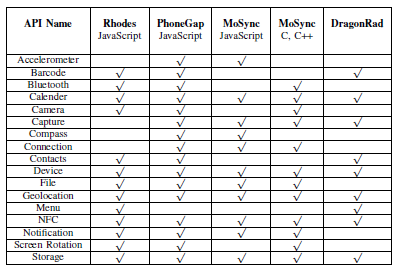
\includegraphics[width=0.7\textwidth]{Bilder/Ergebnis_Sensornutzung_Comparison_of_Cross-Platform_Mob_Dev.PNG}
	\caption{Ergebnis API-Tests aus Palmieri, Singh und Cicchettis Arbeit: Comparison of Cross-Platform Mobile Development Tools aus 2012}
	\label{fig:Ergebnis_API_Test_Publ}
\end{figure}

Wie man in Abbildung \ref{fig:Ergebnis_API_Test_Publ} erkennen kann, schafft es vor allem PhoneGap alle bis auf eine getestete native Funktionalität umzusetzen. Allerdings fanden Palmieri, Singh und Cicchetti heraus, dass vor allem die Frameworks, welche auf JavaScript basieren, deutliche Performance-Probleme haben. Aus diesem Grund raten die Autoren davon ab JavaScript-basierte Frameworks für Anwendungen mit komplexen Funktionalitäten oder im Hintergrund laufende Services zu nutzen. Auch sei die Unterstützung von High-End Grafiken und 3D-Technologien unzureichend\footcite{ComparisonCrossPlatMobDevTools}. 
\\
\\
Eine weitere Arbeit, die sich mit dem Vergleich von hybriden Frameworks beschäftigt hat ist die von Ciman, Gaggi und Gonzo: Cross-Platform Mobile Development: A Study on Apps with Animations aus dem Jahr 2014\footcite{CrossPlatMobDevStudyAnim}. Die Frameworks, die in dieser Arbeit evaluiert wurden sind MoSync, Titanium, JQuery \& JQuery Mobile und PhoneGap. Die Bewertungskriterien, die die Autoren aufstellten sind folgende:

\begin{itemize}
\item Lizenzmodell und Kosten
\item Die Vielfältigkeit und Qualität der verfügbaren APIs
\item Das Angebot an Tutorials
\item Die Größe der Community
\item Die Komplexität des Codes um die vorgegebene Anwendung zu implementieren
\item Die Benutzerfreundlichkeit der IDE des Frameworks
\item Die Liste der unterstützten Geräte
\item Inwieweit die Frameworks das Erstellen einer nativen Benutzeroberfläche unterstützen 
\item Das geforderte Basiswissen im Bereich Programmierung und Technologiekenntnis für jedes Framework
\end{itemize}

Wie man an den Bewertungskriterien oben schon erkennen kann, gaben die Autoren eine Beispiel-Anwendung vor, die mit Hilfe der 4 ausgewählten Frameworks implementiert wurde, um diese gegeneinander zu evaluieren. Um einem Bias entgegenzuwirken wurden für die einzelnen Entwicklungen Entwickler ausgewählt, die mit der jeweiligen Programmiersprache bereits vertraut waren. Die Frameworks wurden anschließend in den oben aufgeführten Kategorien mit Noten von 0 (schlecht) bis 5 (sehr gut) bewertet. Unten stehende Tabelle  (Abbildung \ref{fig:Ergebnis_Framework_Eval_Publ}) zeigt die Ergebnisse:
\clearpage

 \begin{figure}[h]
	\centering
	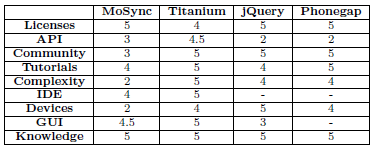
\includegraphics[width=0.65\textwidth]{Bilder/Ergebnis_Framework_Bewertung_Publ_2.PNG}
	\caption{Ergebnis Framework Evaluation von Ciman, Gaggi und Gonzo: Cross-Platform Mobile Development: A Study on Apps with Animations aus 2014}
	\label{fig:Ergebnis_Framework_Eval_Publ}
\end{figure}

Auf Basis oben (Abbildung \ref{fig:Ergebnis_Framework_Eval_Publ}) dargestellten Ergebnisses bewerten die Autoren das Framework Titanium als das Bestes unter den getesteten für Anwendungen mit Animationen. Begründung hierfür ist, dass Titanium Animationen und Übergangseffekte nativ unterstützt und die Performance gut ist und vermuten lässt, dass auch bei komplexeren Anwendungen die Performance noch ausreichend sein wird\footcite{CrossPlatMobDevStudyAnim}. 
\\
\\
In dieser Arbeit sollen ebenfalls, wie bei oben vorgestellten Publikationen, hybride Frameworks direkt miteinander verglichen werden. Um die zu evaluierenden Frameworks auszuwählen, wird zunächst eine Marktanalyse durchgeführt, welche anzeigen soll, welche Frameworks die aktuell attraktivsten sind. Für die Evaluation wird eine Test-Anwendung entwickelt, die mit den ausgewählten Frameworks implementiert werden soll. Diese Anwendung wird zuvor noch als Referenz für zum Beispiel die Performance noch nativ implementiert. Die Anzahl der Frameworks, die mit dieser Anwendung getestet werden ist dabei auf 5 limitiert. Allerdings werden noch weitere Frameworks mit in die Evaluation aufgenommen. Diese können aber nur nach Bewertungskriterien verglichen werden, die nicht direkt mit dem Entwicklungsprozess zusammenhängen. Es wird versucht die Kriterienkataloge der oben vorgestellten Publikationen mittels einer Umfrage unter Anwendungsentwicklern noch zu erweitern.  


\chapter{Grundlagen}

Zunächst werden für ein besseres Verständnis der Arbeit die eingesetzten Materialien und Grundlagen vorgestellt. Zu diesen zählen diverse Hardware, wie das verwendete Smartphone, aber auch Software wie unter anderem die Entwicklungsumgebung oder das verwendete SDK (Software Development Kit) für die native Evaluationsanwendung. Zudem wird eine Einführung in die Begrifflichkeiten wie native und hybride Anwendungsentwicklung gegeben.

\section{Das LG Nexus 5}

Für die Evaluation anhand einer zu entwickelnden Anwendung, welche unter anderem Hardware-Zugriffe auf Sensorik etc. testen soll, steht ein LG Nexus 5 als Gerät zur Verfügung. Das LG Nexus 5 erschien am 31. Oktober 2013 mit der Android-Version 4.4 KitKat. Es verfügt über ein Full HD IPS Display mit einer Bildschirmdiagonalen von 12,70 cm. Die Auflösung beträgt 1920 x 1080 Pixel. Das Smartphone besitzt eine 8 MP Kamera hinten und eine 1,3 MP Front-Kamera. Als Prozessor ist ein Qualcomm Snapdragon 800 mit einer Taktrate von 2,26GHz und 4 Kernen verbaut. Zudem ist das LG Nexus 5 mit folgenden Sensoren ausgestattet: Accelerometer, Gyroskop, Näherungssensor, Magnetometer und Barometer. 

\section{Android}

Android \footcite{Android} ist ein Betriebssystem für mobile Geräte wie Smartphones oder Tablets, ursprünglich entwickelt von der Firma Android, Inc., welche 2005 von Google aufgekauft wurde \footcite{AndroidHistory}. Mobile Anwendungen für Android Systeme werden in der Programmiersprache Java geschrieben und anschließend in Androids eigenes Format DEX (Dalvik Executable Format) konvertiert \footcite{AndroidCookbook}. Die Android UI Guidelines \footcite{AndroidGuidelines} geben Richtlinien für das Design der Benutzeroberfläche von Android Anwendungen vor.
\\
\\
Des Weiteren sind für Android Anwendungen unter anderem noch folgende Grundbedingungen formuliert, an welche sich bei der Planung der Anwendung gehalten wurde: Die Anwendung sollte einfach zu installieren, zu entfernen und zu updaten sein. Sie sollte ansprechend sein und die Anforderungen elegant umsetzen um auch bei vielen Features leicht bedienbar zu bleiben. Wichtig ist, dass die Anwendung stabil, skalierbar, bedienbar ist und angemessen auf Benutzereingaben reagiert.\footcite{AndroidCookbook}

\section{iOS}

iOS ist das native Betriebssystem von Apple für alle Apple Geräte, wie zum Beispiel das iPhone, iPad oder iMacs . Mobile Anwendungen für iOS werden in einer Programmiersprache  namens Swift entwickelt. Apple stellt zum Entwickeln eine eigene IDE zur Verfügung: XCode. Zum Entwickeln von nativen iOS-Anwendungen wird immer ein Apple Computer benötigt\footcite{iOS}. 
\\
\\
Die Richtlinien für das Design grafischer Benutzeroberflächen sind in den 'iOS Human Interface Guidelines' definiert. Die drei primären Grundsätze dabei lauten: Klarheit, Fügsamkeit und Tiefe (Clarity, Deference and Depth)\footcite{iOSGUI}. 

\section{Entwicklungsumgebung}

Das Android SDK ist eine Entwicklungsumgebung für das Android Betriebssystem, welches sich an Entwickler zur Erstellung von Android-Anwendungen wendet und ist für Windows, Linux und Mac OS verfügbar. Es benötigt für viele Hauptfunktionen ein JDK (Java Development Kit) \footcite{AndroidSDK}. Das SDK beinhaltet einen Emulator, der es möglich macht die Anwendung auch ohne angeschlossenes Smartphone zu testen. Als IDE (Integrated Development Environment) wurde Android Studio genutzt, welches 2014 von Google veröffentlicht wurde und so Eclipse als primäre Entwicklungsumgebung für Android Anwendungen ablöste. Android Studio basiert auf der IntelliJ IDEA Community Edition von JetBrains. \footcite{AndroidOP} Es beinhaltet intuitive Tools, die die Erstellung einer grafischen Benutzeroberfläche nach den Android UI Guidelines \footcite{AndroidGuidelines} erleichtern. 

\section{Native Anwendungs-Entwicklung}

Eine native Anwendung ist eine Anwendung, die für eine spezifische Plattform entwickelt wurde und die Schnittstellen dieser Plattform direkt benutzt\footcite{Varianten}. Dadurch kann die Anwendung mit dem Betriebssystem und andere Software, welche auf dem Gerät installiert ist, interagieren. So kann die native Anwendung auch die gerätespezifische Hardware und Software, wie zum Beispiel das GPS oder Kameras verwenden\footcite{nativeApp1}. Ein weiterer Vorteil der nativen Anwendungen ist, dass sie die Ressourcen des Geräts durch die einheitliche Nutzung der Schnittstellen zur Hardware optimal nutzen können\footcite{nativeApp1}. Die plattformspezifischen Bibliotheken bieten zudem alle nötigen Elemente für den Aufbau einer der spezifischen Guidelines entsprechenden Benutzeroberfläche. Eine native Anwendung bringt das maximale  Ergebnis bezüglich Look-And-Feel und Performance\footcite{Varianten}.

\section{Hybride / Cross-Platform Entwicklung}

Eine hybride Anwendung ist prinzipiell wie eine Web Anwendung, nur mit einem leichtgewichtigen nativen Container, welcher es erlaubt, auf native plattformspezifische Funktionalitäten und Hardware zuzugreifen. Wie auch Web Anwendungen werden hybride Anwendungen oft in Skript-Sprachen wie JavaScript, HTML5 und CSS programmiert\footcite{Varianten}. Auf diese Weise entsteht Code, der gemeinsam auf allen Plattformen genutzt werden kann. Dies hat den Vorteil, dass nur eine Anwendung gewartet werden muss und nicht eine pro Plattform, für die die Anwendung herausgegeben werden soll. Als ein Nachteil wird allerdings die Performance genannt, welche unter Umständen, wie zum Beispiel einer erhöhten Nutzung von Hardware-Komponenten, deutlich schlechter als bei der nativen Variante sein soll\footcite{Varianten}. Nachfolgende Abbildung\ref{fig:VariantenAppEntwicklung} beschreibt noch einmal bildhaft den Unterschied zwischen den drei Entwicklungsvarianten: Nativ, Hybrid und Web: 

\begin{figure}[h]
	\centering
	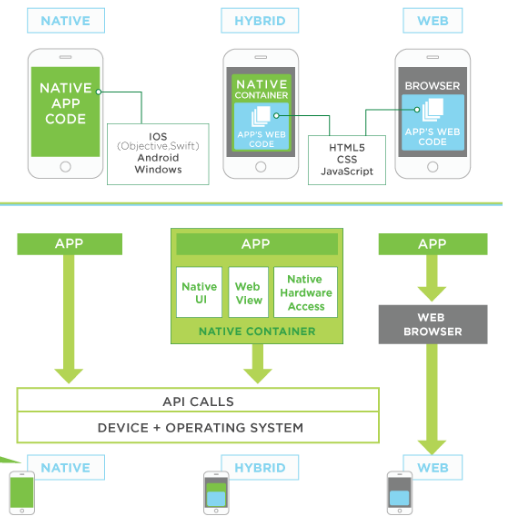
\includegraphics[width=0.5\textwidth]{Bilder/Vergleich_Nativ_Hybrid.PNG}
	\caption{Vergleich: native, hybride und Web Anwendungsentwicklung}
	\label{fig:VariantenAppEntwicklung}
\end{figure}

\section{Sensoren und andere Hardware in Smartphones}

Im folgenden werden die gängigen Sensoren, welche in Smartphones eingebaut sind vorgestellt. Diese Sensoren werden in Anwendungen verwendet, um zum Beispiel die aktuelle Position zu bestimmen oder Feedback in Form von Vibrationen zu geben. 

\subsection{Accelerometer und Gyroskop}

Das Accelerometer, oder auch der Beschleunigungssensor, misst die Beschleunigung in X-, Y- und Z-Achsenrichtung. Unter Beschleunigung wird die Änderung der Geschwindigkeit zur Zeit verstanden. Im physikalischen Sinne ist jede Form von Änderung einer Bewegung, auch eine Abnahme der Geschwindigkeit oder Schwenken in eine andere Richtung, eine Beschleunigung. Das Gyroskop misst hingegen die rotatorische Geschwindigkeit, also Drehbewegungen. Zusammen mit dem Accelerometer erkennt das Smartphone so Bewegungsänderungen und kann darauf reagieren\footcite{AndroidWiki}. Die Ausrichtung der 3 Achsen von einem Smartphone ist in folgender Abbildung\ref{fig:Achsenausrichtung} dargestellt:

\begin{figure}[h]
	\centering
	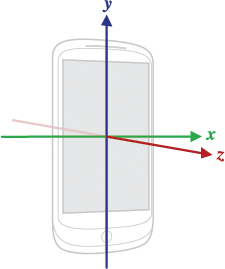
\includegraphics[width=0.5\textwidth]{Bilder/Axis_device.PNG}
	\caption{Schematisches Achsenmodell; Entnommen von: www.droidwiki.de/wiki/G-Sensor}
	\label{fig:Achsenausrichtung}
\end{figure}

\subsection{GPS}

GPS ist die Abkürzung für Global Positioning System und beschreibt ein System zur globalen Positionsbestimmung mit Hilfe von Satelliten. Smartphones mit GPS besitzen einen GPS-Chip, mit denen sie ihre Position auf 5-10 Meter genau bestimmen können\footcite{AndroidWiki}. Der GPS-Sensor ist relevant für zum Beispiel Navigations-Anwendungen. 

\subsection{Näherungssensor und Umgebungslichtsensor}

Der Näherungssensor bei Smartphones besteht üblicherweise aus einem Fotowiderstand und er dient zusammen mit dem Umgebungslichtsensor zur Messung der Helligkeit des Umgebungslichtes. Die Aufgabe des Näherungssensors ist es in der Regel, schnelle Änderungen der Umgebungshelligkeit festzustellen. Der Umgebungslichtsensor misst anhand des photoelektrischen Effekts das Umgebungslicht und passt daraufhin die beispielsweise automatisch die Display-Helligkeit an\footcite{AndroidWiki}. 

\subsection{Vibration}

Um auf Benutzereingaben eine Rückmeldung in Form eines Vibrationsfeedbacks zu geben, sind Vibrationsmotoren in Smartphones verbaut. Diese sind über die API des jeweiligen Betriebssystems ansprechbar. Gerade bei Geräten mit Touchscreen und ohne mechanische Tastatur kann ein solches Feedback es dem Benutzer vereinfachen, seine Eingabe als erfolgt zu erkennen\footcite{AndroidWiki}. 

\subsection{Magnetometer}

Ein  Magnetometer misst die magnetische Flussdichte und kann so bestimmen, wo sich der magnetische Norden befindet. Im Inneren des magnetometers befindet sich eine metallische Platte, welche unter Strom gesetzt wird. Durch das Wirken der Lorentzkraft auf diese Platte, deren Stärke abhängig von der Stärke des vorhandenen Magnetfeldes ist, wird diese verschoben. Das Magnetometer misst optisch oder elektrisch wie weit sich die Platte verschoben hat. Mit Hilfe des Magnetometers im Smartphone lassen sich Kompass-Anwendungen und Anzeigen der Blickrichtung auf Karten-Anwendungen realisieren\footcite{AndroidMag}. 
\chapter{Anforderungsanalyse}

blablabla 

\section{Problemanalyse}

Zur Evaluation der ausgewählten Frameworks wird eine Anwendung designed, welche diverse Hardware- und Software-Funktionalitäten eines Smartphones nutzt und testet. Diese Anwendung wird zunächst als Referenz nativ für die Android Plattform(X) in Android Studio entwickelt um anschließend mit 5 ausgewählten Frameworks neu umgesetzt zu werden. Auf diese Weise wird überprüft und evaluiert, welche Funktionalitäten mit welchen Frameworks nutzbar sind und welcher eventuelle Mehr-Aufwand entsteht. Zudem wird bei der Neuumsetzung mit den ausgewählten Frameworks überprüft, inwieweit sich die GUI der nativen Anwendung im Material Design(X) nachstellen lässt. 
\\
\\
Als weitere Grundlage für die Evaluation der Frameworks dient eine Umfrage, die an Studierende der Fachhochschule Dortmund mit Erfahrung im Bereich Anwendungsentwicklung gestellt wurde. Mit Hilfe dieser Umfrage werden weitere Kriterien ermittelt, die Entwicklern wichtig bei der Arbeit mit einem Framework sind.
\\
\\
Aus oben genannten Hardware- und Software-Funktionalitäten und den durch die Umfrage ermittelten Kriterien wird eine Evaluations-Matrix erstellt, welche während der Umsetzung der Referenz-Anwendung mit den ausgewählten Frameworks gefüllt wird. Aus dieser Matrix sollen anschließend die Möglichkeiten, sowie die Vor- und Nachteile, die ein Framework bietet, abgelesen werden können.

\section{Funktionale und nichtfunktionale Anforderungen}

Zunächst werden die funktionalen Anforderungen, also Anforderungen, die sich direkt auf die Funktionalitäten der Referenzanwendung beziehen, und die nichtfunktionalen Anforderungen definiert. Die funktionalen Anforderungen werden in folgende Bereiche unterteilt: Zugriffsmöglichkeiten und Nutzung von Hardware-Komponenten wie zum Beispiel Sensoren und Kamera, die Möglichkeiten bei der Gestaltung der grafischen Benutzeroberfläche, ... Danach werden noch die nichtfunktionalen Anforderungen beschrieben, welche in folgende Kategorien unterteilt sind: ...

\subsection{FA: Nutzung von Hardware-Komponenten}

\begin{itemize}

\item Accelerometer
\begin{list}{}{}
\item Es muss möglich sein, die Accelerometer-API anzusprechen und so Daten vom Accelerometer abzugreifen und nutzen zu können. 
\end{list}

\item Vibration
\begin{list}{}{}
\item Es muss möglich sein die Vibrationsfunktion des Smartphones anzusprechen und nutzen zu können.
\end{list}

\item Kamera
\begin{list}{}{}
\item Sowohl die Front- als auch die Rückkamera des Smartphones müssen über das Framework ansprechbar und benutzbar sein. 
\end{list}

\item GPS
\begin{list}{}{}
\item Das GPS des Smartphones muss nutzbar sein, um die aktuelle Position des Gerätes ermitteln und anzeigen lassen zu können. 
\end{list}

\item Speicher
\begin{list}{}{}
\item Es muss möglich sein Dateien in den lokalen Speicher des Smartphones zu schreiben, lesen und auch wieder zu löschen.
\end{list}

\item Netzwerknutzung
\begin{list}{}{}
\item Es muss möglich sein in einer mit dem zu testenden Framework gebauten Anwendung Zugriff zum Internet zu bekommen und gegebenenfalls Dateien herunterladen zu können.
\end{list}

\item Lagesensor/Gyroskop
\begin{list}{}{}
\item Es soll geprüft werden, ob der Lagesensor von einer Anwendung, welche mit dem zu testenden Framework entwickelt wurde, ansprechbar ist um die Lage des Smartphones ermitteln zu können.
\end{list}

\item Näherungssensor
\begin{list}{}{}
\item Es soll geprüft werden, ob der Näherungssensor eines Smartphones muss weiterhin nutzbar ist.
\end{list}

\item Notifications
\begin{list}{}{}
\item Es soll überprüft werden, ob Notifications über eine in dem zu testenden Framework entwickelten Anwendung ausgegeben werden können.
\end{list}

\item Kommunikation
\begin{list}{}{}
\item Es soll getestet werden, ob Kommunikationen via Bluetooth und WiFi für Gerät-zu-Gerät- und Gerät-zu-Netzwerk-Kommunikation möglich sind.
\end{list}

\item Speicher
\begin{list}{}{}
\item Es soll geprüft werden, ob Dateien in den lokalen Speicher des Smartphones geschrieben, gelesen und auch wieder gelöscht werden können. Hierbei soll zusätzlich überprüft werden, welche Datenhaltungsformate unterstützt werden.
\end{list}

\end{itemize}

\subsection{FA: Die grafische Benutzeroberfläche}

Ein natives Look-And-Feel einer mobilen Anwendung bedeutet, dass die grafische Benutzeroberfläche dem Benutzer das Gefühl einer nativen Anwendung vermittelt. Die ausgewählten Frameworks müssen hierzu die Möglichkeit bieten, native Bedienelemente bei der Entwicklung von Anwendungen zu verwenden. Es muss möglich sein die Oberfläche einer Anwendung nach dem Design-Standard des entsprechenden Betriebssystems (Android, iOS) aufzubauen. Hier wird im Falle des Betriebssystems Android der aktuelle Design-Standard ‚Material Design‘ (X) gefordert. Um dies zu testen ist es notwendig in die Test-Anwendung gängige Bedienelemente wie zum Beispiel Action-Bars, Floating Buttons und Navigationselemente zu integrieren.

\subsection{FA: Betriebssysteme}

Für jedes zu untersuchende Framework soll ermittelt werden, für welche Plattformen sich Anwendungen damit entwickeln lassen. Der Fokus liegt hierbei auf den mobilen Betriebssystemen Android und iOS, da diese den Großteil des Marktes ausmachen (vgl. Kapitel X). Hierbei soll auch berücksichtigt werden, wie viele und welche ältere Versionen der Betriebssysteme vom entsprechenden Framework unterstützt werden und inwieweit eine Anwendung abwärtskompatibel ist. Auch soll untersucht werden wie viel Zeit die Hersteller der Frameworks durchschnittlich benötigen um auf ein Betriebssystemupdate seitens iOS und Android zu reagieren.
\\\\
Zudem wird ermittelt auf welchen Betriebssystemen die Frameworks für die Entwicklung installiert werden können.  

\subsection{FA: Sicherheit}

Bezüglich der Sicherheitsaspekte von mobilen Anwendungen soll überprüft werden, ob und inwieweit das Rechtemanagement der jeweiligen Plattform (Android, iOS) nativ unterstützt wird. Dies beinhaltet unter anderem die Regelung der Zugriffe auf Gerätefunktionen wie Speicher oder die Kameras. Auch wird untersucht, ob es Möglichkeiten zur Hinterlegung von Sicherheitszertifikaten gibt und ob ein eigener privater Zertifikatspeicher eingerichtet werden kann. 

\subsection{FA: Interoperabilität/Erweiterbarkeit}

Unter dem Sammelpunkt Interoperabilität und Erweiterbarkeit finden sich Prüfungen, die sich auf eine mögliche Anpassbarkeit der Frameworks und die Nutzung von Bibliotheken von Fremdanbietern beziehen. In diesem Zuge wird auch ermittelt, ob sich die Frameworks in gängige IDEs, wie zum Beispiel Visual Studio oder Eclipse integrieren lassen und ob es eine Auswahl an Programmiersprachen gibt, mit denen entwickelt werden kann.

\subsection{FA: Tests und Performance}

Bei der Evaluierung von Frameworks für Crossplatform- beziehungsweise hybrider Anwendungs-entwicklung wird auch untersucht inwiefern die einzelnen Frameworks Werkzeuge zum Schreiben und Durchführen von (automatisierten) Tests selbst anbieten oder unterstützen. Die Anwendung, die als Evaluationshilfe im Rahmen dieser Arbeit entwickelt wird, soll zudem Möglichkeiten bieten die Performance der Cross-Platform-Anwendungen mit einer nativen Anwendung zu vergleichen. Hierzu muss die zu entwickelte Test-Anwendung Messungen der Reaktionszeiten der Anwendung ermöglichen. 

\subsection{NFA: Hersteller}

Als eine der nichtfunktionalen Anforderungen wird die Bedeutsamkeit der Hersteller/Anbieter der einzelnen Frameworks recherchiert. Hierzu zählen Attribute wie Unternehmensgröße, Bekanntheitsgrad (Score), Produktpalette und Einsätze. Zudem werden in diesem Rahmen auch die Entwicklungsstadien der Frameworks näher durchleuchtet und Fragen hinsichtlich der aktuellen Version und der Anzahl vergangener Updates beantwortet. Auch wird untersucht, in welchem Umfang versprochene Funktionalitäten bereits umgesetzt wurden und welche Erweiterungen und Verbesserungen in Planung sind.  

\subsection{NFA: Support und Community}

Die Untersuchung des Umfangs des Hersteller-Supports findet unter Berücksichtigung folgender Gesichtspunkte statt: Werden Tutorials und Beispiellösungen für verschiedene Problemstellungen geboten? Werden Online-Schulungen und/oder Schulungen mit Anwesenheit angeboten? Gibt es eine Dokumentation, die regelmäßig gepflegt wird? Gibt es ein Forum, in dem Fragen gestellt werden können, die von einem Support-Team des Herstellers beantwortet werden? 
\\\\
Zusätzlich zum Hersteller-Support soll auch die Größe der jeweiligen Community betrachtet werden. Die Größe wird dabei anhand der Internetpräsenz bemessen. 

\subsection{NFA: Entwicklung}

Ein wichtiger Faktor bei der Evaluation von Frameworks für hybride und Cross-Platform-Anwendungsentwicklung ist der Entwicklungsprozess mit den entsprechenden Frameworks. Unter diesem Aspekt werden unter anderem die Leichtigkeit der Installation und der Benutzung der Frameworks verglichen. Gemessen wird dies an der notwendigen Einarbeitungszeit und der Zeit die insgesamt für Installation und Einrichtung aller für die Entwicklung notwendigen Werkzeuge benötigt wird. Hier fließt auch der Umfang der Bibliotheken, welche die Frameworks mit sich bringen, in Form folgender Fragestellungen ein: Welche Bausteine für die Entwicklung werden angeboten und was muss alles selbst implementiert werden? Zentrales Kriterium ist auch der Anteil des plattformübergreifend nutzbaren Codes am Gesamtcode, hier am Beispiel der Funktionstest-Anwendung, welche als Werkzeug zur Evaluation dient. 

\subsection{NFA: Lizenz und Kosten}

Bei der Evaluation werden auch etwaige Kosten und Lizenzmodelle der zu untersuchenden Frameworks betrachtet. Hier werden die einzelnen Frameworks hinsichtlich etwaiger Kaufpreise, Monats- oder Jahreslizenzpreise und Kosten für Support sowie Minor und Major Upgrades untersucht. 

\section{Abgrenzungskriterien}

Im Rahmen dieser Projektarbeit wird eine Marktanalyse durchgeführt, um die 5 aktuell relevantesten Frameworks aus dem Bereich hybrider und Cross-Platform-\\Anwendungsentwicklung auszuwählen. Die als Evaluationswerkzeug dienende \\Funktionstest-Anwendung wird einmal nativ als Referenz und anschließend nur mit diesen 5 ausgewählten Frameworks implementiert. Weitere Frameworks werden nur aufgrund ihrer Spezifikationen und Literatur untersucht. Aufgrund der zur Verfügung stehenden Hardware und Software wird die native Variante der mobilen Anwendung, welche als Evaluationswerkzeug entwickelt wird, ausschließlich in Android für ein Android Smartphone entwickelt. Somit werden sich sämtliche Teile der Evaluation, welche mit Hilfe der Funktionstest-Anwendung erarbeitet werden, nur auf die Android-spezifischen Bereiche der Frameworks beziehen können. Bei der Evaluation des nativen Look-And-Feel anhand des GUI-Designs wird sich an den aktuellen Richtlinien für das Material Design von Android orientiert.
\chapter{Marktanalyse} \label{Marktanalyse}

Wie schon in der Anforderungsanalyse (Kapitel \ref{Anforderungsanalyse}) beschrieben, werden die 3 aktuell relevantesten Frameworks für hybride, bzw. Cross-Platform-Anwendungsentwicklung ausgewählt, um diese mit einer Funktionstest-Anwendung zu evaluieren. Die Vorgehensweise sieht dabei wie folgt aus: Zunächst wurden grundsätzliche Kriterien definiert, die die zu evaluierenden Frameworks erfüllen müssen. Nachfolgend wurde eine Liste der infrage kommenden Frameworks erstellt. Diese Frameworks wurden anschließend mit verschiedenen Tools auf ihre aktuelle Relevanz überprüft. Nur die Relevantesten wurden dann anschließend genauer betrachtet um eine abschließende Auswahl zu treffen.
\\
\\
Bevor eine allgemeine Liste aktuell verfügbarer Frameworks aufgestellt wurde, wurden folgende Kriterien festgelegt, welche auf jeden Fall von den Frameworks erfüllt werden müssen, um bei dieser Evaluation Berücksichtigung zu finden: Die Frameworks müssen mehr als eine Plattform bedienen, und 2 dieser Plattformen müssen Android und iOS sein, da diese den größten Marktanteil besitzen (siehe Kapitel \ref{Einleitung}). Wobei Android einen durchschnittlichen Marktanteil von ca. 75\% und iOS von ca. 18\% über die vergangenen 4 Jahre besaß\footcite{Statista}.
Folgende Frameworks konnten nach oben genannten Kriterien ausfindig gemacht werden:
\\
\begin{itemize}
\item React Native
\item CodenameOne
\item Xamarin
\item Ionic
\item Intel XDK
\item Onsen UI
\item Kendo UI
\item Mobile Angular UI
\item Cordova
\item PhoneGap
\item J2ObjC
\item AppGyver
\item ViziApps
\item Monocross
\item Marmalade
\item Corona
\item Agate
\item Apache Flex
\item AppConKit
\end{itemize}

Um die 3 aktuell relevantesten Frameworks zu ermitteln, wurden folgende Medien genutzt: Mit dem Google AdWords Keyword Planer\footcite{KeyWordPlaner} wurden die durchschnittlichen Suchanfragen nach dem Namen des jeweiligen Frameworks pro Monat über den Zeitraum des letzten Jahres ermittelt. Hierbei ergab sich bei den oben aufgeführten Frameworks folgende Verteilung:
\clearpage
\begin{figure}[h]
	\centering
	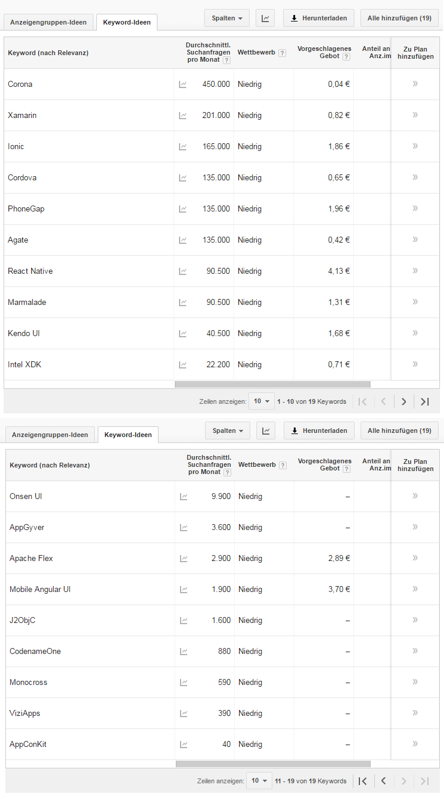
\includegraphics[width=0.6\textwidth]{Bilder/Durchschnittliche_Suchanfragen_gesamt.PNG}
	\caption{Durchschnittliche Suchanfragen bei Google, ermittelt mit Google AdWords Keyword Planer}
	\label{fig:Suchanfragen1}
\end{figure}

\clearpage
Zusätzlich wurden mit Hilfe von Google Trends\footcite{GoogleTrends} die Popularität der einzelnen Frameworks im Zeitverlauf visualisiert, um zu verdeutlichen welche Frameworks in letzter Zeit an Interresierten dazugewonnen haben. Die Ergebnisse werden bei Google Trends in Relation zum totalen Suchaufkommen gesetzt. Die Trends sind für einzelne Regionen sowie für die ganze Welt verfügbar. In diesem Fall wurden die weltweiten Trends für die Frameworks ausgewertet. Da sich nur 5 Suchbegriffe gleichzeitig in einem Graphen gegenüberstellen lassen, wurden immer 4 Frameworks 'Corona', welches in der vorherigen Untersuchung mit dem Keyword Planer\footcite{KeyWordPlaner} die meisten monatlichen Suchanfragen aufwies, als Referenz gegenübergestellt. Da einige Frameworks Namen haben, die auch in völlig anderen Zusammenhängen gesucht werden können, wie zum Beispiel 'Marmalade', wurde als Suchkategorie 'Computer und Elektronik' ausgewählt.
\\
\\
\begin{figure}[h]
	\centering
	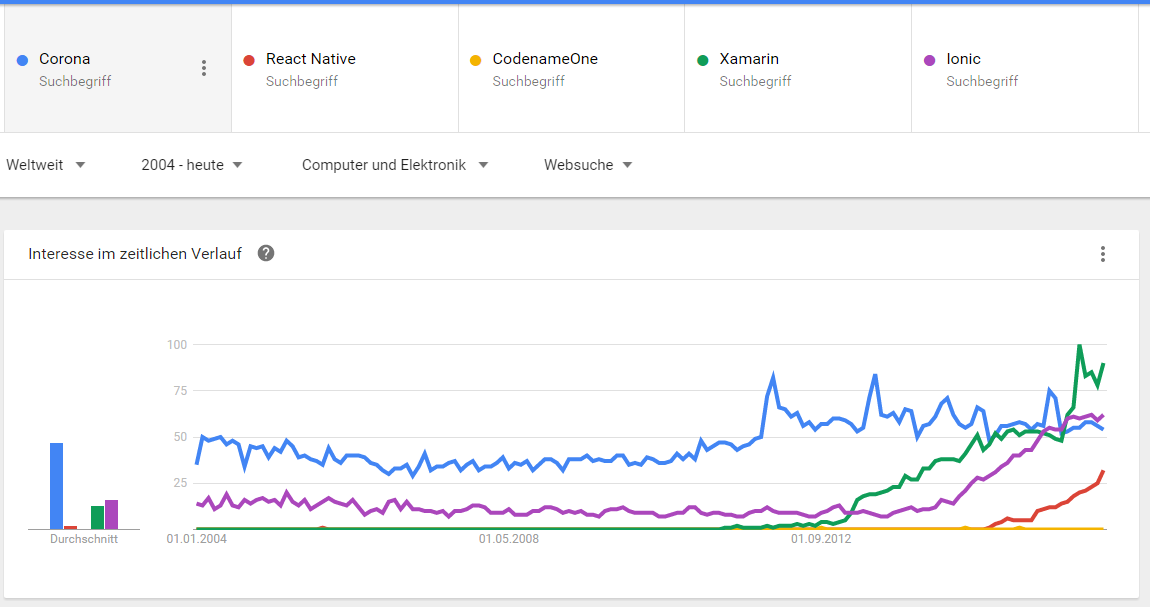
\includegraphics[width=0.8\textwidth]{Bilder/trends_1.PNG}
	\caption{Google Trends: React Native, CodenameOne, Xamarin und Ionic im Vergleich zu Corona}
	\label{fig:Trends1}
\end{figure}
\begin{figure}[h]
	\centering
	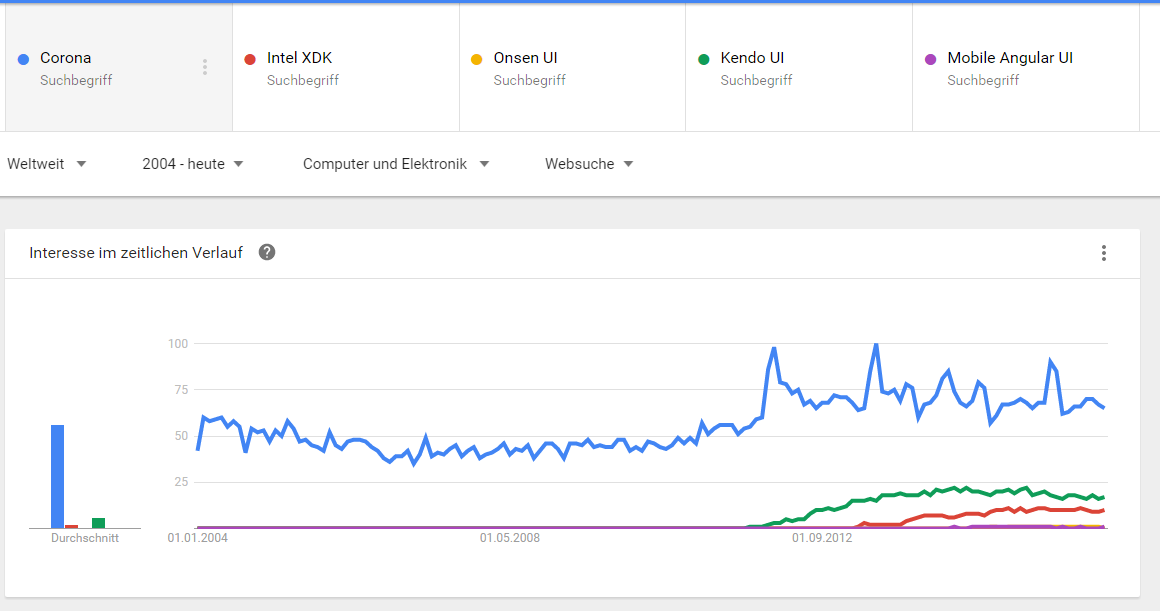
\includegraphics[width=0.8\textwidth]{Bilder/trends_2.PNG}
	\caption{Google Trends: Intel XDK, Onsen UI, Kendo UI und Mobile Angular UI im Vergleich zu Corona}
	\label{fig:Trends2}
\end{figure}
\begin{figure}[h]
	\centering
	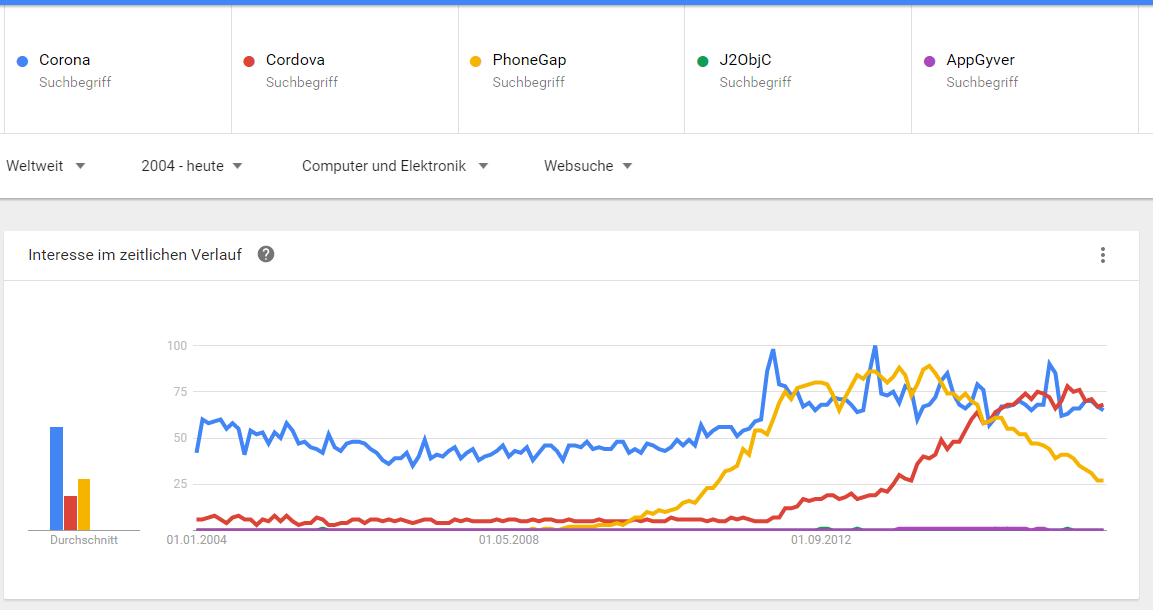
\includegraphics[width=0.8\textwidth]{Bilder/trends_3.PNG}
	\caption{Google Trends: Cordova, PhoneGap, J2ObjC und AppGyver im Vergleich zu Corona}
	\label{fig:Trends3}
\end{figure}
\begin{figure}[h]
	\centering
	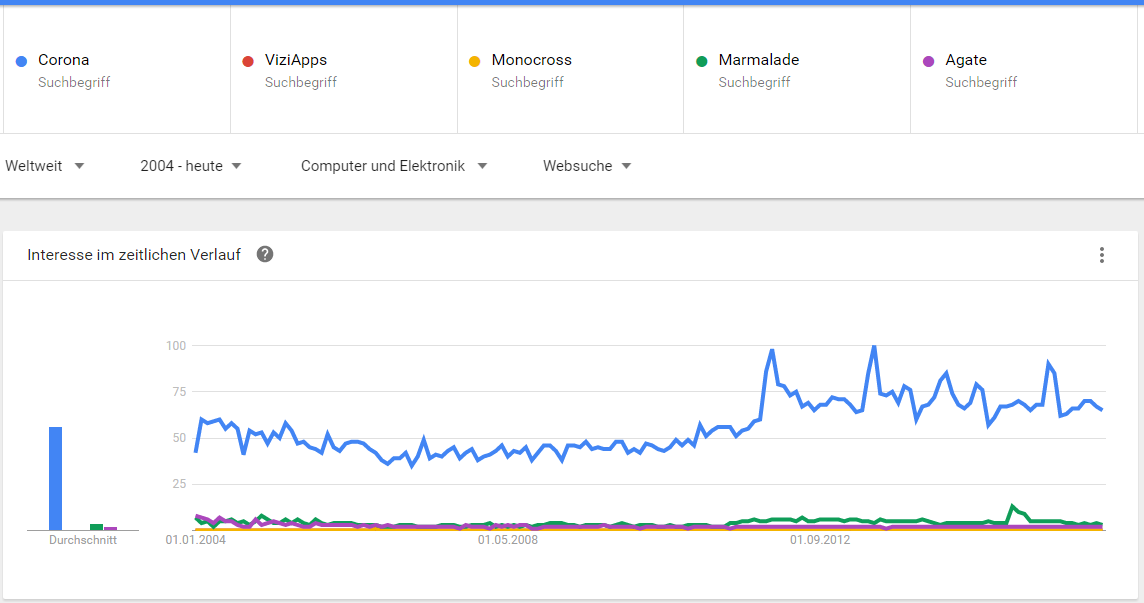
\includegraphics[width=0.8\textwidth]{Bilder/trends_4.PNG}
	\caption{Google Trends: ViziApps, Monocross, Marmalade und Agate im Vergleich zu Corona}
	\label{fig:Trends4}
\end{figure}
\begin{figure}[h]
	\centering
	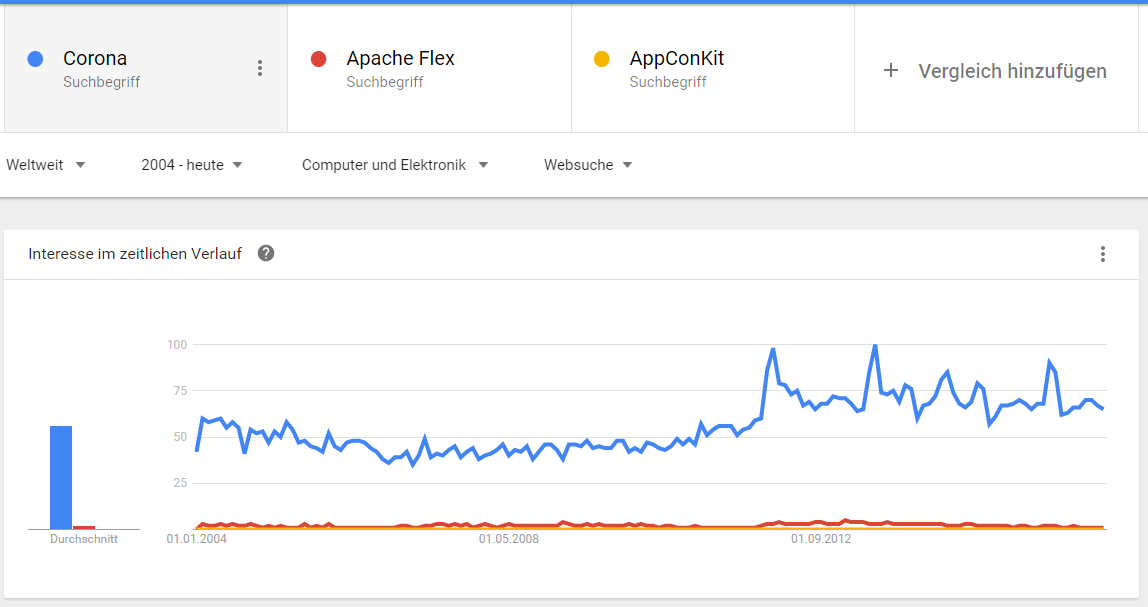
\includegraphics[width=0.8\textwidth]{Bilder/trends_5.PNG}
	\caption{Google Trends: Apache Flex und AppConKit im Vergleich zu Corona}
	\label{fig:Trends5}
\end{figure}
\clearpage
Aus oben beschriebenen und dargestellten Auswertungen ergeben sich zunächst folgende 5 Frameworks in der engeren Auswahl, welche durch die Implementierung einer Funktionstest-Anwendung evaluiert werden sollen:
\begin{itemize}
\item Corona
\item Xamarin
\item Cordova
\item PhoneGap
\item Ionic
\end{itemize}
Aufgrund der vergleichsweise sehr geringen Repräsentation des Frameworks Corona auf GitHub (ca. 2000 Repositories im Vergleich zu um die ca. 30.000 Einträge zu Ionic oder React Native) wird dieses von den oben aufgelisteten Frameworks hintenangestellt\footcite{GitHubTrending}. Nach weiteren Recherchen über diese 5 Frameworks stellte sich noch heraus, dass es sich bei Cordova um eine Weiterentwicklung des Frameworks PhoneGap handelt. Dies schlägt sich auch in den Google Trends nieder, wie man in Abbildung \ref{fig:Trends3} erkennen kann. Aus diesem Grund wird ausschließlich Cordova evaluiert, der Vorgänger PhoneGap bleibt außen vor. Für die Liste der zu evaluierenden Frameworks ergibt sich daraus, dass an die Stelle von PhoneGap nun 'React Native' tritt. 
\\
\\
Das Framework Cordova bietet keine Mittel für die Realisierung einer grafischen Benutzeroberfläche und für das Framework Ionic ist für sämtliche Hardware-Nutzung das Einbinden von Cordova-Plugins notwendig. Aus diesen Gründen werden diese beiden Frameworks in dieser Arbeit kombiniert betrachtet, als 2 Bausteine eines Frameworks sozusagen. So ergeben sich für die Evaluation in dieser Arbeit folgende Frameworks:
\begin{itemize}
\item Xamarin
\item Ionic mit Cordova-Pugins
\item React Native
\end{itemize}
Diese Frameworks werden nachfolgend etwas näher vorgestellt. 

\section{Xamarin} \label{chpXamarin}

Das Xamarin Framework verspricht native Anwendungen für Windows Phone, iOS und Android entwickeln zu können basierend auf einer C\# Codebase. Konkret gesprochen verspricht es eine native UI, nativen API Zugang und native Performance Xamarin kommt mit der eigenen IDE 'Xamarin Studio', es ist allerdings auch möglich Xamarin Anwendungen mit der IDE 'Visual Studio' zu entwickeln. Die Benutzeroberfläche muss bei Xamarin Anwendungen allerdings für jede Plattform separat implementiert werden\footcite{EinerFuerAlles}. 

\section{Cordova} \label{chpCordova}

Cordova von Apache ist ein Open Source Framework für Cross-Platform mobile Anwendungsenwicklung. Das Framework ist kostenlos nutzbar und unterstützt Standard Web Technologien wie HTML5, CSS3 und JavaScript für die Entwicklung. Die Anwendungen werden in sogenannten Wrappern ausgeführt, die die API der jeweiligen Plattform ansprechen um so Zugang zu unter anderem Sensoren zu bekommen. Die Plattformen, die von Apache Cordova unterstützt werden sind: Android, Blackberry 10, iOS, OS X, Ubuntu, Windows und Windows Phone 8\footcite{Cordova}. 

\section{Ionic}

Das Ionic Framework basiert auf AngularJS, was wiederum ein clientseitiges JavaScript-Webframework ist\footcite{AngularJS}. Entsprechend werden Ionic Anwendungen ebenfalls in JavaScript, HTML5 und CSS3 geschrieben. Auf diese Weise wird bei diesem Framework die gemeinsame Code-Basis geschaffen. Ionic bietet eine nativ wirkende GUI, für Hardware-Anbindungen, wie zum Beispiel das Nutzen von Sensoren, müssen allerdings Cordova (Kapitel  \ref{chpCordova}) PlugIns genutzt werden\footcite{Ionic}. 

\section{React Native}

React Native nutzt die Bibliothek React von Facebook zur Entwicklung für die Plattformen Android, iOS und die Universal Windows Platform. Programmiert werden React Native Anwendungen in JavaScript und HTML. Der Code wird anschließend in native Quelldateien übersetzt, weshalb React Native verspricht native Komponenten ohne großen Aufwand einbinden zu können und flüssige Animationen zu ermöglichen\footcite{EinerFuerAlles}.
\chapter{Aufstellen der Bewertungskriterien für die Analyse} \label{Bewertungskriterien}

Für die Evaluierung der Frameworks wird zunächst ein Katalog mit Bewertungskriterien angefertigt, anhand dessen die einzelnen Frameworks bewertet werden. Der Katalog besteht dabei aus Kriterien, die alle in Kapitel \ref{Anforderungsanalyse} vorgestellten Anforderungen an die Frameworks überprüfen sollen. Zusätzlich werden noch Kriterien aufgenommen, die durch eine Umfrage ermittelt wurden. 
\\
\\
Oben erwähnte Umfrage richtete sich an (ehemalige) Studierende der Fachhochschule Dortmund, welche angaben, bereits Erfahrungen in der mobilen Anwendungsentwicklung gesammelt zu haben. Die Fragestellung der Umfrage lautete: „Welche Kriterien halten Sie für wichtig in der Entwicklung mit Frameworks für hybride, bzw. Cross-Platform-Anwendungen?“ (E-Mail siehe Anhang) Die Befragten antworteten hierauf mit einem Freitext, indem sie die für sich wichtigen Kriterien zur Bewertung von Frameworks aufzeigten. Diese Kriterien wurden in einem Dokument (siehe CD-ROM im Anhang) gesammelt und Mehrfachnennungen entsprechend gekennzeichnet. Ein Kriterium, welches von mehreren Befragten als wichtig beschrieben wurde, bekommt bei der Evaluation eine höhere Gewichtung zugeschrieben, als ein Kriterium, welches nur von einem Befragten genannt wurde. Aus dieser Zusammenfassung der ermittelten Bewertungskriterien wurde anschließend eine Matrix (siehe Abbildung \ref{fig:Bewertungskriterien_1}-\ref{fig:Bewertungskriterien_3}) erstellt. Der Grad der Erfüllung eines Kriteriums wird an der Anzahl an Punkten zu erkennen sein, die vergeben werden. Hier ist eine Skala von 1 bis 5 (gar nicht bis voll erfüllt) vorgesehen. Wobei hier zu jedem Kriterium zunächst definiert werden muss, was „voll erfüllt“ bedeutet. Neben diesen Kriterien wird es auch Kriterien geben, welche nur mit „vorhanden“ und „nicht vorhanden“ bewertet werden können.

\section{Kategorie Kosten und Lizenz} 

In der Kategorie Kosten und Lizenz gibt es einen Sonderfall bei dem Punkt „Lizenzmodell“. Es ist hier nicht möglich eine konkrete Abstufung von „gut“ nach „schlecht“ in 5 Kategorien zu schaffen, da verschiedene Lizenzmodelle verschiedene Vor- und Nachteile aufweisen können. So wird sich darauf beschränkt, lediglich eine kurze Beschreibung des jeweiligen Lizenzmodells, sofern es eins gibt, zu formulieren. 
\\
\\
Die Punkte „Fixkosten“, „Lizenzkosten“ und „Supportkosten“ werden in 5 Abstufungen von „gratis“ bis „teuer“ unterteilt. Die exakten Geldwerte für die Grenzen der Abstufungen werden sich aus dem günstigsten und teuersten Preis, welche sich zu den Frameworks ermitteln lassen, ergeben.

\section{Kategorie Support und Community}

Bezüglich des Punktes 2)a) „Support/Wartung vom Hersteller“ (siehe Abbildung \ref{fig:Bewertungskriterien_1}) wird der Umfang des Supports pro Framework ermittelt und anhand dessen die Abstufung vorgenommen. Dies umfasst zum Beispiel telefonischen Support, ein Ticket-System oder ein moderiertes Forum. Die Qualität von Punkt 2)b) „Dokumentation“ wird unter anderem am Umfang der Dokumentation selber und am Update-Zyklus bemessen, d.h. wie schnell wird die Dokumentation entsprechend Änderungen am Framework aktualisiert? Bei der Untersuchung der Größe der Community werden, falls vorhanden, das Framework eigene Forum und weitere Entwicklerforen nach Anzahl Threads mit Themen, die sich auf das jeweilige Framework beziehen, durchleuchtet. Das Schulungsangebot wird sowohl nach Qualität als auch nach Quantität beurteilt: Das bedeutet, dass unterschieden wird, ob nur Online- oder auch Anwesenheitsschulungen angeboten werden. Hierbei spielt es auch eine Rolle an wie vielen unterschiedlichen Standorten und wie häufig Schulungen angeboten werden. Zudem wird der Angebotsumfang an Schulungen hinsichtlich einer Aufteilung von Anfänger- bis Spezialschulungen bewertet.

\section{Kategorie Entwicklung}

In der Kategorie „Entwicklung“ (siehe Abbildung \ref{fig:Bewertungskriterien_1}) werden für die Leichtigkeit der Installation und Benutzung des Frameworks Punkte von 1 bis 5 vergeben: 1 bedeutet kompliziert und aufwändig und 5 bedeutet automatisiert und intuitiv. Als „Einarbeitungszeit“ wird in diesem Falle die Zeit von der Fertigstellung der Installation bis nach dem Schreiben der ersten funktionierenden Seite der Anwendung angesehen. Hier gilt je kürzer, desto besser. Bei Punkt 3)c) „plattformübergreifend nutzbarer Code“ inwieweit der mit dem jeweiligen Framework erzeugte Code plattformübergreifend nutzbar ist, beziehungsweise wie hoch der Anteil des plattformspezifischen Codes ist. Hier gilt entsprechend, je mehr Code plattformübergreifend nutzbar ist, desto besser. Unter „Umfang Bibliotheken/Templates“ wird verstanden, wie viele Bausteine mit dem Framework sozusagen mitgeliefert werden, die einzelne Funktionalitäten kapseln und einfach in den Code zu integrieren sind.

\section{Kategorie Hersteller}

Die „Bekanntheit/Größe des Herstellerunternehmens“ des jeweiligen Frameworks wird anhand der Unternehmensgröße, des Bekanntheitsgrads, der Produktpalette und Einsätze der Produkte gewertet. Bei dem Punkt „Entwicklungsstadium des Frameworks“ (siehe Abbildung \ref{fig:Bewertungskriterien_1}) wird in die Wertung mit einbezogen, ob sich das Framework noch in einer Beta-Version befindet, oder es schon ein Release gibt. Zudem wird betrachtet, wie viele Updates und Bugfixes bereits vorgenommen wurden und wie viel von dem was das Framework laut Hersteller leisten soll bereits umgesetzt oder noch in Planung ist. Eine „Ja“-„Nein“-Unterscheidung gibt es bei dem Punkt „Weiterentwicklung des Frameworks“. Hierbei ist positiv zu bewerten, wenn das Framework nachweislich noch weiterentwickelt werden soll, um mit den Änderungen und der Weiterentwicklung der einzelnen Plattformen mithalten zu können.

\section{Kategorie OS-Versionen}

„Reaktionszeit auf OS-Update“ (siehe Abbildung \ref{fig:Bewertungskriterien_1}) beschreibt die Zeit, die benötigt wurde um nach einem Update eines Betriebssystems, wie zum Beispiel Android, das Framework entsprechend anzupassen oder zu erweitern. Mit dem Punkt „Abwärts-kompatibilität“ wird bewertet, bis zu welcher OS-Version das Framework anwendbar ist. Hier ist zum Beispiel für Android nicht ohne Bedeutung, dass weiterhin Version 4.x unterstützt wird, die unter den Android Versionen immer noch einen großen Marktanteil annehmen\footcite{AndroidMarktanteil4}. Desweiteren werden bewertet, auf wievielen unterschiedlichen Plattformen das Framework installiert und entwickelt werden kann und für wieviele mobile Plattformen entwickelt werden kann. 

\begin{figure}[h]
	\centering
	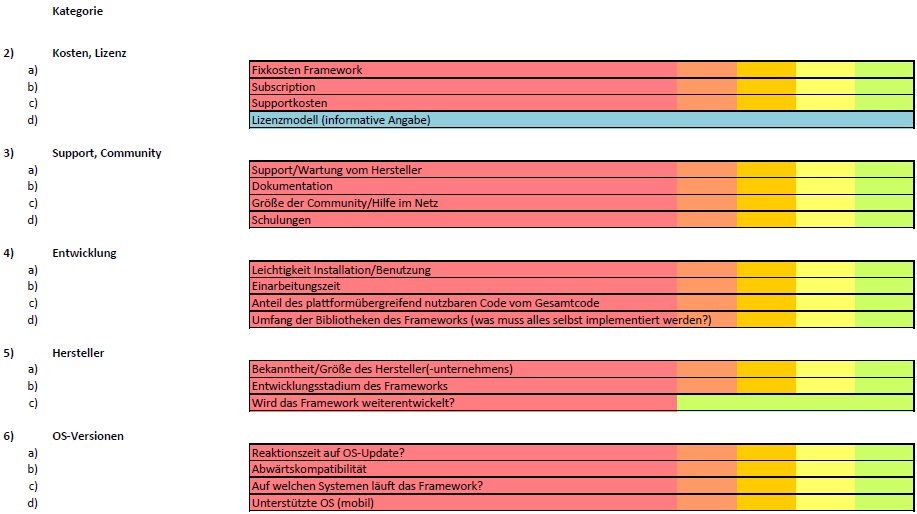
\includegraphics[width=1\textwidth]{Bilder/Bewertungsmatrix_1.PNG}
	\caption{Matrix der Bewertungskriterien, Teil 1}
	\label{fig:Bewertungskriterien_1}
\end{figure}

\section{Funktionsumfang}

In der Kategorie Funktionsumfang wird eine "Ja"-"Nein"-Unterscheidung bei der Fragestellung, welche Sensoren angesprochen und genutzt werden können, vorgenommen. Informationen darüber, welche Sensoren mit dem jeweiligen Framework genutzt werden können, bieten die jeweiligen Spezifikationen. Zusätzlich wird der Funktionsumfang der in Kapitel \ref{Marktanalyse} ausgewählten 3 Frameworks mit der Funktionstest-Anwendung praktisch getestet. So kann bei diesen Frameworks zusätzlich eine Bewertung über die Anwendbarkeit vergeben werden. Die Sensoren, die getestet werden sind: Der Beschleunigungssensor, der Lagesensor mit dem Gyroskop, das GPS, der Näherungs-sensor, das Magnetometer und das Barometer (siehe Abbildung \ref{fig:Bewertungskriterien_2}). 
\\
\\
Neben den oben beschriebenen Sensoren werden auch Funktionen wie die Benutzung der Front- und Rückkamera, der Zugriff auf das Dateisystem des Smartphones und Notifications getestet. Hier bekommen die in Kapitel \ref{Marktanalyse} ausgewählten Frameworks wie bei den Sensoren eine erweiterte Bewertung. Bei Punkt 6)6) "Kommunikation" fließt in die Bewertung mit ein, welche und wieviele unterschiedliche Kommunikationswege genutzt werden können, wie zum Beispiel Bluetooth oder WiFi. 

\section{GUI-Design}

Nur einen "Ja"-"Nein"-Unterschied gibt es bei den Punkten 7)1) "GUI-Designer" und 7)3) "integrierter Emulator", welcher schlicht besagt, ob diese Werkzeuge in dem jeweiligen Framework enthalten sind oder nicht (siehe Abbildung \ref{fig:Bewertungskriterien_2}). Punkt 7)2) Bei "Umfang der verfügbaren (nativen) UI-Elemente" wird getestet, welche unterschiedlichen Elemente des Android Material Designs einfach einsetzbar bar sind und für welche Elemente aufwändige oder weniger aufwändige Imports von Bibliotheken notwendig sind. Zudem wird der Aufwand bewertet entsprechende UI-Elemente in die Anwendung zu integrieren. 

\section{Interoperabilität und Erweiterbarkeit}

Punkte 8)1) "Webserviceaufrufe" und 8)2) "Bibliotheken von Fremdanbietern" werden mit einer "Ja"-"Nein"-Unterscheidung bewertet (siehe Abbildung \ref{fig:Bewertungskriterien_2}), d.h. es wird über-prüft, ob Webserviceaufrufe und Einbindung fremder Bibliotheken mit dem jeweiligen Framework möglich sind. Mit Punkt 8)4) "Support-Tools" wird bewertet, ob das Framework Support-Tools zur Verfügung stellt. Bei Punkt 8)3) "Integration in IDEs" wird ermittelt, wieviele unterscheidliche IDEs für die Entwicklung mit dem jeweiligen Framework einsetzbar sind, d.h. in wieviele IDEs das Framework integriert werden kann. 
\clearpage

\begin{figure}[h]
	\centering
	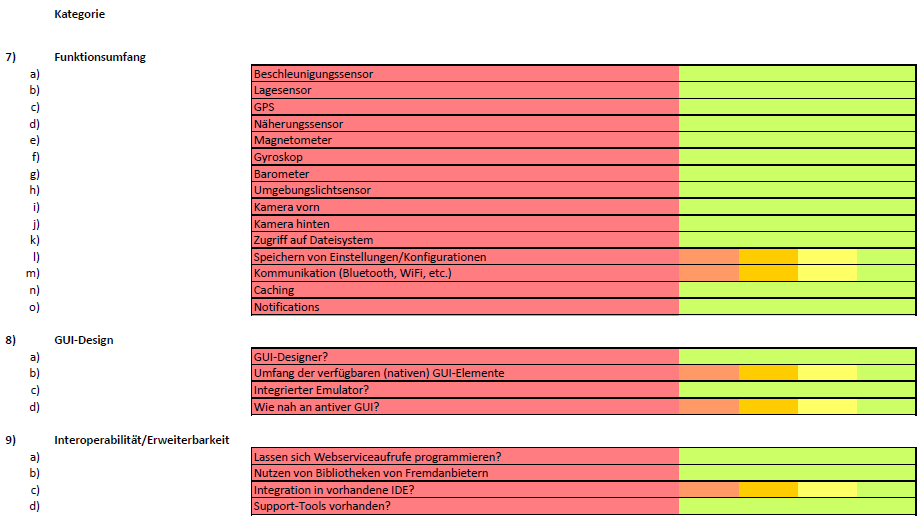
\includegraphics[width=1\textwidth]{Bilder/Bewertungsmatrix_2.PNG}
	\caption{Matrix der Bewertungskriterien, Teil 2}
	\label{fig:Bewertungskriterien_2}
\end{figure}

\section{Tests}

Bei den beiden Punkten 9)1) "Automatische Tests" und 9)2) "Test-Tools" (siehe Abbildung \ref{fig:Bewertungskriterien_3}) wird allein mit einer "Ja"-"Nein"-Unterscheidung bewertet, ob automatische Tests möglich und Test-Tools mit dem Framework ausgeliefert werden. 

\section{Performance}

Bei dem Bewertungskriterium "Performance" wird eine Abstufung entsprechend der Größe des Performance-Unterschieds zur nativen Anwendung vorgenommen. Auch wird die Größe der gebauten Installationspakete verglichen. 

\section{Sicherheit}

In dieser Kategorie werden folgende Fragestellungen beantwortet: 11)1): Wird das Rechtemanagement der jeweiligen Plattform nativ unterstützt? 11)3): Kann man Sicherheitszertifikate hinterlegen? 11)4): Kann ein eigener Zertifikatspeicher eingerichtet werden? 11)5): Werden VPN Verbindungen nativ umgesetzt (siehe Abbildung \ref{fig:Bewertungskriterien_3})? Zudem werden informative Angaben zu der Realisierung des Zugriffs auf Geräte-funktionen wie Speicher oder Kamera gemacht.  

\begin{figure}[h]
	\centering
	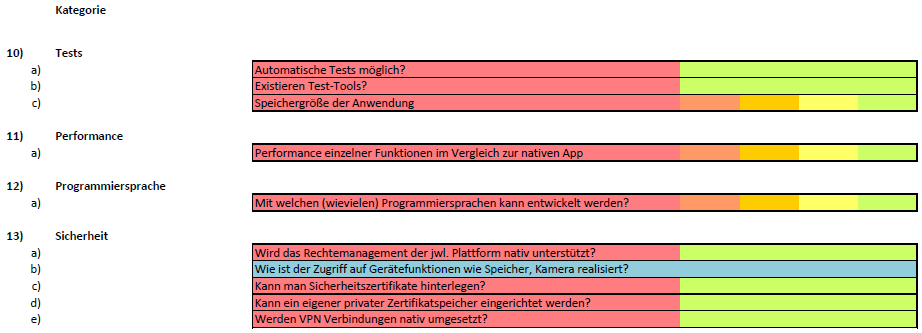
\includegraphics[width=1\textwidth]{Bilder/Bewertungsmatrix_3.PNG}
	\caption{Matrix der Bewertungskriterien, Teil 3}
	\label{fig:Bewertungskriterien_3}
\end{figure}
\chapter{Planung der Funktionstest-Anwendung}

Anhand des durch die Anforderungsanalyse festgelegten Rahmens müssen nun Entscheidungen bezüglich Tests der Datenhaltung, der Sensoren und des Designs der Benutzeroberfläche und Benutzerführung getroffen werden. In den folgenden Abschnitten werden diese Entscheidungen behandelt. Wie schon in Kapitel (X) erläutert, wird die Funktionstest-Anwendung zunächst als Referenz für die Plattform Android nativ entwickelt. Entsprechend wird sich unter anderem bei der graphischen Benutzeroberfläche an den Android Guidelines orientiert, welche im Folgenden näher erläutert werden. 

\section{GUI Design}

Die Android GUI-Guidelines beschreiben das Design-Prinzip von Android Anwendungen als 'Material Design'. Das Design, die Oberfläche soll materiell, greifbar wirken. Der Gebrauch von gewohnten, greifbaren Attributen soll dem Benutzer helfen schnell Funktionen und Bedienelemente zu verstehen. Licht, Oberflächenbeschaffenheiten und Bewegung beschreiben wie einzelne Objekte Der GUI miteinander interagieren und in welcher Relation sie zueinander stehen. Die fundamentalen Elemente print-basierten Designs wie die Typographie, Raum, Farbe und Metaphorik dienen nicht nur optischen Highlights sondern sie formen Hierarchien, Bedeutung und Fokus. Im Material Design soll so eine Oberfläche geschaffen werden, die als 'bold and graphic' bezeichnet wird. Diese zeichnen gezielte Farbkombinationen, bewusst eingesetzte Leerräume und eine groß-skalierte Typographie aus. Die Bewegungen einzelner Bedienelemente sollen bedeutungsvoll sein und dazu dienen den Fokus auf sich zu ziehen um den Benutzer auf intuitive Art und Weise durch Anwendungen navigieren zu lassen. Auf diese weise soll auch klar verständliches Feedback auf Benutzereingaben gegeben werden\footcite{AndroidOnlineGuidelines}. 
\\
\\
Die Android Design-Guidelines betonen folgende 3 Prinzipien:

\begin{itemize}
\item Enchant Me
\begin{list}{}{}
\item Mit 'Enchant Me' ist gemeint, dass zum Beispiel vorsichtig platzierte Animationen und gut gesetzte Soundeffekte dafür sorgen, dem Benutzer ein Gefühl von Mühelosigkeit vermitteln sollen. Dem Benutzer soll die Möglichkeit gegeben werden anstelle von Buttons und Menüs direkt mit einzelnen Objekten in der Anwendung interagieren zu können. Dies soll die kognitive Anstrengung gering halten und die Anwendung ansprechender gestalten. Mit der Möglichkeit optionaler Anpassungen soll der Benutzer der Anwendung eine persönliche Note geben können. Zudem sollte eine Anwendung lernen, was die Präferenzen des Benutzers sind und entsprechende häufig verwendete Funktionen in den Vordergrund heben und leicht erreichbar anbieten\footcite{AndroidDesignPrinciples}.
\end{list}
\item Simplify My Life
\begin{list}{}{}
\item Unter 'Simplify My Life' zählt unter anderem, dass darauf geachtet werden sollte, kurze Sätze mit einfachen Wörtern zu verwenden, da lange Sätze eher eine abschreckende Wirkung haben. Zudem sollten, wo es nur möglich ist, Bilder und Symbole anstelle von Text genutzt werden, um Ideen zu erklären. Einstellbare, bzw. konfigurable Funktionen sollten voreingestellt sein, um den Benutzer vor der ersten Nutzung der Anwendung einen Einstellungsmarathon zu ersparen. Es sollte dem Benutzer aber die Möglichkeit gegeben werden die Konfigurationen einfach nach seinem Geschmack anzupassen. Für eine bessere Übersichtlichkeit sollte auch darauf geachtet werden nicht zu viele Optionen und Informationen gleichzeitig anzuzeigen und so die Anzeige zu überladen und den Benutzer zu überfordern. Verschiedene Bereiche in einer Anwendung sollen verschieden aussehen und es sollen Übergänge zwischen Bereichen geschaffen werden, die deren Beziehungen untereinander verdeutlichen. Auf diese Weise soll der Benutzer die Orientierung in der Anwendung nicht verlieren. Des weiteren soll darauf geachtet werden, dass Formen, hinter denen bestimmte Funktionen stecken, ausschließlich für diese Funktionen genutzt werden, frei nach dem Motto 'Was gleich aussieht, sollte gleich funktionieren'. Als letztes wird unter dem Punkt 'Simplify My Life' aufgeführt, dass der Benutzer nur dann bei der Bedienung unterbrochen werden soll, wenn diese Unterbrechung dazu dient wirklich kritische Informationen zu übermitteln. Wegen unnötiger Details sollte der Benutzer nicht gestört werden\footcite{AndroidDesignPrinciples}. 
\end{list}
\item Make Me Amazing
\begin{list}{}{}
\item 'Make Me Amazing' besagt unter anderem, dass man versuchen sollte visuelle und haptische Muster und Gesten aus anderen Android Anwendungen in die eigene Anwendung mit einfließen zu lassen. So hat es der Benutzer nochmals leichter sich in der neuen Anwendung zurecht zu finden. Werden von dem Benutzer Korrekturen verlangt, so sollten diese ihm freundlich vermittelt werden. Wenn etwas schief läuft, sollen klare ver-ständliche Wiederherstellungsanweisungen gegeben werden, auf technische Details sollte verzichtet werden. Alles was im Hintergrund ohne den Benutzer ablaufen kann, sollte dort geschehen. Auf sämtlichen Benutzereingaben sollte es ein Feedback geben, auch wenn es nur ein leichtes leuchten ist. Können mehrere komplizierte Arbeitsschritte zusammengefasst werden, sollte man dies tun und es dem Benutzer als Bündel zur Verfügung stellen. Ein Beispiel hierfür wären einige kombinierte Filter für die Fotonachbereitung. Zu guter Letzt wird darauf hingewiesen, dass darauf geachtet werden soll, dass die wichtigsten Funktionen der Anwendung leicht zu finden und zu benutzen sein sollen. Als gutes Beispiel dient hier der Pause-Button bei Musik-Anwendungen oder der Auslöser bei der Kamera\footcite{AndroidDesignPrinciples}. 
\end{list}
\end{itemize}

Für die geplante Funktionstest-Anwendung bedeutet dies, dass zumindest die Standard 'Material Design' Bedien- und Navigationselemente integriert werden sollten. Das Android Studio bietet einige Kompositionen an Elementen für die Seitenerstellung an, an diese sollte sich gehalten werden, da sie dem 'Material Design'-Prinzip entsprechen. Zu diesen Elementen zählen zum Beispiel der 'Navigation Drawer' für die Navigation zwischen einzelnen Seiten der Anwendung oder der 'Floating Action Button', ein runder Button, welcher im Vordergrund über dem Inhalt der Anwendung schwebt. Er verschwindet nicht, wenn hinter ihm in der Seite gescrollt wird und steht so immer zur Verfügung. Auch die 'Bottom Navigation Bar' darf in der Anwendung nicht fehlen, sie ist eine einheitliche globale Navigation durch das Android Betriebssystem. Auch eine 'App Bar' soll am oberen Rand des Displays integriert werden. Diese stellt Shortcuts und weitere Menüverwaltungsmöglichkeiten zur Verfügung. In unten stehender Abbildung (X) ist eine leere Beispielseite einer Android Anwendung im 'Material Design' Abgebildet. Man erkennt deutlich die 'Bottom Navigation Bar' am unteren Rand der Seite, die 'App Bar' am oberen Rand und den 'Floating Action Button' in der rechten unteren Ecke. 

\begin{figure}[h]
	\centering
	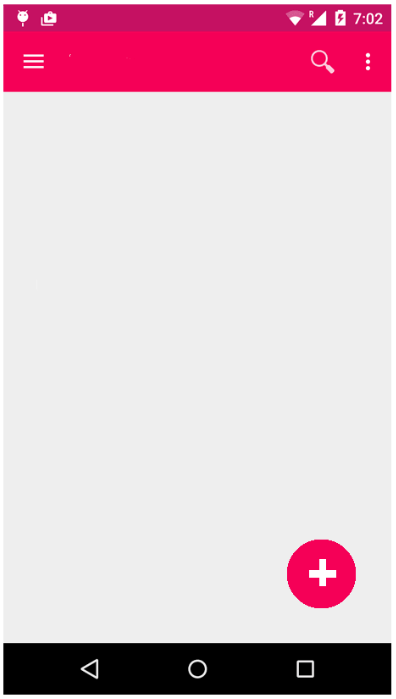
\includegraphics[width=0.35\textwidth]{Bilder/Material_Design_Blank_Page.PNG}
	\caption{Beispiel einer leeren Seite einer Android Anwendung im 'Material Design'}
	\label{fig:Material_Design}
\end{figure}

\section{Hardwarezugriffe}

Android bietet für den Zugriff auf Sensoren auf der API-Ebene im Paket android.hardware Unterstützung für eine Vielzahl von Sensoren an. In der Sensor-Klasse ist für jeden Sensortyp eine Konstante definiert, wie zum Beispiel \\ Sensor.TYPE\_ACCELEROMETER für den Beschleunigungssensor. Einige dieser Sensoren repräsentieren dabei tatsächliche Hardware-Sensoren, andere wiederum sind Software-basierte Sensoren, deren Messungen auf einer Kombination von Hardware-Sensoren basieren(Buch Android5 Kapitel 15 (X)). Da es Smartphones gibt die pro Sensortyp mit mehreren Sensoren ausgestattet sein können, gibt es pro Typ in Android einen sogenannten Default-Sensor und eine Sensorliste, in welcher alle verfügbaren Sensoren eines Typs enthalten sind. Über den Reporting-Mode kann eingestellt werden, wann der Sensor Daten an die Anwendung liefern soll. Hier gibt es unter anderem die Möglichkeit kontinuierlich Daten übermitteln zu lassen oder nur bei Änderungen in der Messung(Buch Andorid-Quick-API-References Kapitel 8 (X)). 
\\
\\
Für die Standortbestimmung bietet Android eine eigene, separate API. Aufgrund datenschutzrechtlicher Bestimmungen müssen bei der Standortbestimmung Berechtigungen direkt vom Benutzer eingeholt werden um diese nutzen zu können. Die eigentliche Bestimmung des Standortes kann auf 3 unterschiedliche Weisen geschehen: einmal via GPS (X), via WiFi Zugangspunkten oder Sendemasten oder als dritte Möglichkeit passiv über die Standortanfragen anderer auf dem Smartphone befindlicher Anwendungen(Buch Andorid-Quick-API-References Kapitel 8 (X)). 
\\
\\
Für die Interaktion mit den Kameras des Smartphones bietet Android ein reichhaltiges Set an APIs. Ähnlich zur Standortbestimmung werden auch bei der Nutzung der Kameras Berechtigungen gefordert. Der Entwickler kann im Manifest seiner Android Anwendung einstellen, ob die Kameranutzung für die Anwendung notwendig oder optional ist. Eine Anwendung, für die die Kameranutzung notwendig ist, kann über Google Play nicht auf Geräten ohne Kamera installiert werden. Android stellt zudem noch einige Konfigurationsparameter bereit, über die sich zum Beispiel die Qualität des JPEG-Bildes oder Blitzfunktionen voreinstellen lassen(Buch Andorid-Quick-API-References Kapitel 9 (X)). 

\section{Speicher}

Für das Speichern von Daten gibt es je nach Zweck und Datengröße unterschiedliche Möglichkeitnen bei Android. So können zu jeder Activity über sogenannte Shared Preferences Konfigurationen gespeichert werden. Die auf diese Weise gespeicherten Daten sind Privateigentum der jeweiligen Activity, keine andere Activity oder gar Anwendung hat Zugriff darauf(Buch Android5 Kapitel 12 (X)). 
\\
\\
Bei größeren Datenmengen und für direktes Lesen und Schreiben in Dateien ist der Shared Preferences Ansatz eher ungeeignet. Hier werden Java-IO-Klassen wie zum Beispiel der FileInpuStream oder der FileOutputStream verwendet. Als Speicherorte gibt es den internen Speicher (Internal Storage) und den externen Speicher (External Storage)(Buch Android5 Kapitel 12 (X)):

\begin{itemize}
\item Interner Speicher:
\begin{list}{}{}
\item Der interne Speicher ist immer vorhanden, die enthaltenen Daten sind Anwendungs-spezifisch. Dies bedeutet, dass nur die Anwendung, der die Daten gehören Zugriff auf diese besitzt. Andere Anwendungen können diese Daten nicht nutzen. Wird die Anwendung deinstalliert, so werden in diesem Zuge auch alle Daten in ihrem internen Speicher gelöscht(Buch Android5 Kapitel 12 (X)). 
\end{list}
\item Externer Speicher:
\begin{list}{}{}
\item Daten im externen Speicher können von mehreren Anwendungen genutzt werden. Der externe Speicher kann in Form einer einsteckbaren SD-Karte vorliegen, aber auch der Speicher des Smartphones hat einen Bereich, der als 'External Storage' angesprochen werden kann. Je nach Android-Version gibt es allerdings Unterschiede bezüglich der Zugriffsrechte und der Unterteilung des Speichers(Buch Android5 Kapitel 12 (X)). 
\end{list}
\end{itemize}

In der Funktionstest-Anwendung soll die Verwendung des externen Speichers innerhalb des Smartphones, also ohne extra SD-Karte integriert werden. Hierbei soll sowohl das Lesen als auch das Schreiben von Dateien umgesetzt werden. 
\chapter{Objektorientierte Analyse und Design} \label{OOAOOD}

Im Folgenden wird die objektorientierte Analyse, kurz OOA, beschrieben. In der Analyse geht es darum, die Anforderungen an die Anwendung unter anderem grafisch in Diagrammen zu erfassen und zu beschreiben, mit dem Ziel, ein objektorientiertes Analyse-Modell als Ergebnis zu erhalten. Anschließend wird im objektorientierten Design, kurz OOD, das in der Analyse erstellte Modell weiterentwickelt und in eine konkrete Softwarearchitektur überführt, die dann als direkte Implementierungsvorlage dient\footcite{SWTBalzert}.
\\
\\
Zunächst werden in der objektorientierten Analyse das statische Modell und das dynamische Modell beschrieben. In der Regel wird das statische Modell anhand eines Klassendiagramms beschrieben, in dem alle notwendigen Klassen und Beziehungen dargestellt werden, um die in der Anforderungsanalyse definierten Anforderungen an die Anwendung umzusetzen. Die dynamischen Modelle beschreiben hingegen Abläufe bei der Nutzung der Anwendung. 

\section{Dynamisches Modell (OOA)}

Die Interaktionen des Benutzers mit der Funktionstest-Anwendung werden in folgendem Use-Case-Diagramm (Abbildung \ref{fig:Use_Case}) dargestellt. Links ist der allgemeine Benutzer dargestellt. Der Benutzer der Funktionstest-Anwendung muss eine Auflistung der Sensoren angezeigt bekommen, die er testen kann. Er muss die Kamera des Smartphones benutzen können, das heißt, dass er Fotos schießen und diese auch speichern können soll. Entscheidet sich der Benutzer dazu Sensoren zu testen, so kann er folgende Aktivitäten durchführen: Der Benutzer kann durch Bewegungen seines Smartphones den Beschleunigungssensor und mit diesem zusammen den Lagesensor und das Gyroskop testen. Er kann sich auf einer Karte seinen aktuellen Standort anzeigen lassen. Mit Hilfe des im Smartphone integrierten Magnetometers soll sich der Benutzer den magnetischen Nordpol anzeigen lassen können. Als letzten Sensor soll der Benutzer auch den Näherungssensor testen können. Die Fotos, die der Benutzer mit der Kamerafunktion aufgenommen hat, soll er sich auch später ansehen und auch wieder löschen können. Als letztes gibt es noch eine Funktion, mit der sich der Benutzer das Logging der Anwendung in einem Textdokument anzeigen zu lassen kann und eine Funktion, die es dem Benutzer ermöglicht das Farbschema des Designs der Anwendung zu ändern.  

\begin{figure}[h]
	\centering
	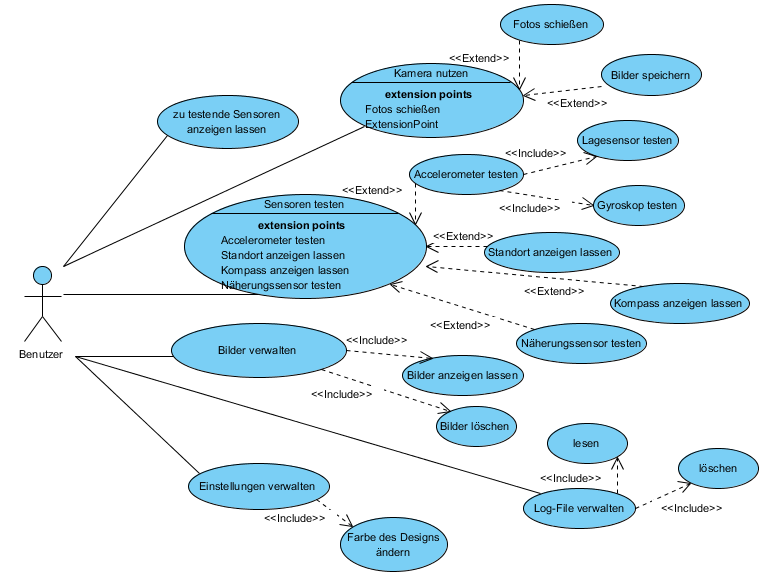
\includegraphics[width=1\textwidth]{Bilder/Use_Case.PNG}
	\caption{Funktionstest-Anwendung: Use-Case Diagramm}
	\label{fig:Use_Case}
\end{figure}

\section{Statisches Modell (OOA)} \label{OOAStatMod}

Die Funktionstest-Anwendung wird einmal nativ und anschließend mit 3 unterschiedlichen Frameworks entwickelt, was bedeutet, dass sie mit unterschiedlichen Programmiersprachen implementiert werden muss (siehe Kapitel \ref{Marktanalyse}). Dabei sind nicht alle dieser Programmiersprachen objektorientiert und die vorgegebene Architektur der einzelnen Frameworks ist zu diesem Zeitpunkt noch unbekannt. Aus diesem Grund empfiehlt sich an dieser Stelle kein UML Klassendiagramm. Anstelle dessen werden in einem Diagramm die einzelnen Funktionen und die Navigation zu diesen dargestellt (siehe Abbildung \ref{fig:Diagram_1}). So können Hierarchien und Tiefe der Anwendung auch ohne Klassendiagramm analysiert und gezeigt werden.  

\begin{figure}[h]
	\centering
	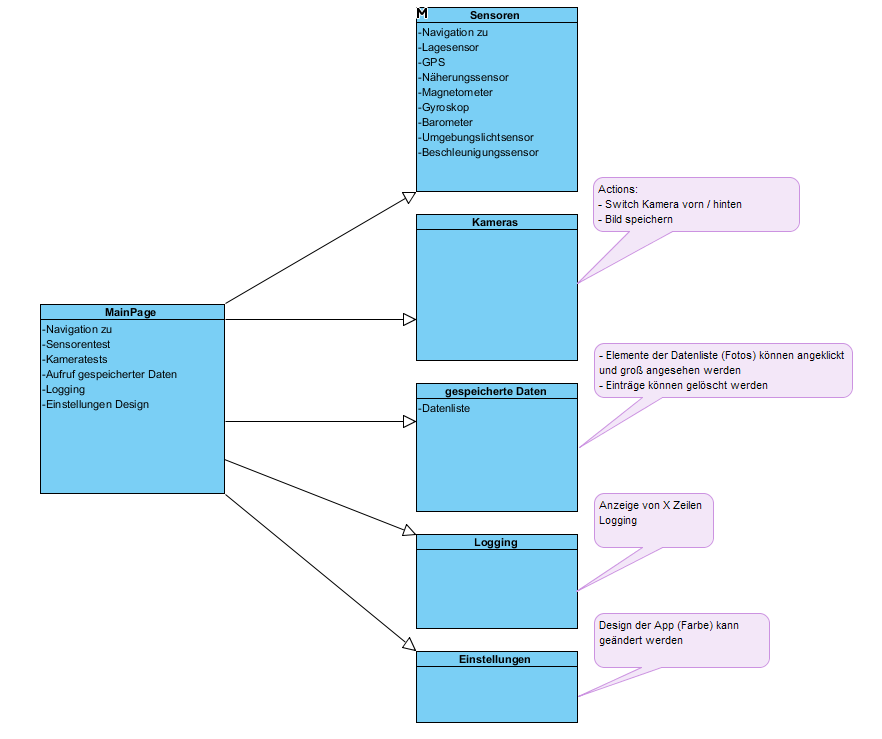
\includegraphics[width=1\textwidth]{Bilder/Diagram_1.PNG}
	\caption{Funktionstest-Anwendung: Navigation Hauptmenü und Beschreibung der einzelnen Funktionen}
	\label{fig:Diagram_1}
\end{figure}

Wie in Abbildung \ref{fig:Diagram_1} zu sehen ist, soll die Anwendung von der 'MainPage' aus starten. Die 'MainPage' ist ein Navigationsmenü, von dem aus der Benutzer zu folgenden Seiten navigieren kann: Zur Sensorliste, zur Kamerafunktion, zu der Seite, welche die vom Benutzer gespeicherten Daten verwaltet, zum Logging-Output und zu einer Einstellungsseite. Die Seite mit der Sensorliste stellt dabei selbst wieder ein Navigationsmenü dar. Navigiert der Benutzer vom Hauptmenü zur Kamerafunktion, so soll er da die Möglichkeit haben, zwischen der Front- und der Rückkamera des Gerätes auszuwählen und Fotos zu schießen. Geschossene Fotos können gespeichert werden. Ein weiterer Menüpunkt des Hauptmenüs führt den Benutzer zur Verwaltung seiner gespeicherten Fotos. Dort soll er durch klicken auf ein Foto dieses vergrößert angezeigt bekommen. Zudem hat er dort die Möglichkeit ausgewählte Bilder wieder zu löschen. Im Menüpunkt 'Logging' wird dem Benutzer das von der Anwendung generierte Logfile angezeigt und im Menüpunkt 'Einstellungen' kann der Benutzer zwischen vorkonfigurierten Farbdesigns für die Anwendung auswählen. 
\\
\\
Im Navigationsmenü der Sensoren kann der Benutzer zu weiteren Funktionen der Anwendung navigieren, wie in Abbildung \ref{fig:Diagram_2} zu sehen ist: 


\begin{figure}[h]
	\centering
	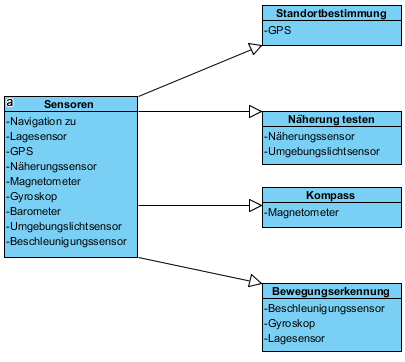
\includegraphics[width=0.6\textwidth]{Bilder/Diagram_2.PNG}
	\caption{Funktionstest-Anwendung: Navigation Sensortests und Beschreibung der einzelnen Funktionen}
	\label{fig:Diagram_2}
\end{figure}
\clearpage
Die 4 Funktionstestseiten, zu denen der Benutzer navigieren kann sind einmal die Standortbestimmung, der Näherungstest, die Kompassanzeige und die Bewegungserkennung (siehe Abbildung \ref{fig:Diagram_2}). Bei der Standortbestimmung wird der GPS-Sensor des Smartphones angesprochen und getestet. Auf dem Display soll eine Weltkarte angezeigt werden mit einem Marker an der Stelle an der der Benutzer sich mit seinem Smartphone befindet. Es soll in die Karte hineingezoomt werden können, damit Ermittlung des Standorts durch das GPS besser überprüft werden kann. Für den Näherungstest werden der Näherungssensor und der Umgebungslichtsensor angesprochen. Hier soll auf dem Display des Smartphones Feedback gegeben werden, sobald sich ein Gegenstand nähert. Das Magnetometer wird bei der Kompassanzeige getestet. Hier bekommt der Benutzer eine Kompassnadel zu Gesicht, welche zum magnetischen Nordpol zeigt. Unter dem Menüpunkt 'Bewegungserkennung' werden der Beschleunigungssensor, das Gyroskop und gegebenenfalls der Lagesensor getestet, sollte es einen separaten geben. 

\section{Datenhaltung (OOD)}

Entsprechend der in Kapitel \ref{Anforderungsanalyse} definierten Anforderungen und der in Kapitel \ref{PlanungAnwendung} ausgearbeiteten Funktionen der Funktionstest-Anwendung sollen die Fotos, die der Benutzer mit der Kamerafunktion schießt auf dem Smartphone gespeichert werden. Sie sollen im 'External Storage' abgelegt werden. So soll es auch möglich sein aus anderen Anwendungen heraus auf diese Bilder zuzugreifen und sie auf andere Medien zu übertragen. Als Speicherformat für die Fotos wird 'JPG' verwendet. Für die Fotos soll die Anwendung vorher einen eigenen Ordner mit dem Namen 'Feature\_Test\_App' anlegen.

\section{Die grafische Benutzeroberfläche} \label{OOAOODGUI}

Bei der Erstellung des Prototyps für die grafische Benutzeroberfläche wurde darauf geachtet möglichst einige der Standardelemente des 'Material Designs' \ref{PlanungAnwGUI} zu verwenden, welche auch für die native Entwicklung im Android Studio zur Verfügung gestellt werden.
\\
\\
Die Startseite der Anwendung ist das Hauptmenü (Siehe Kapitel \ref{OOAStatMod}). Hier wird der in Kapitel \ref{PlanungAnwGUI} erwähnte 'Navigation Drawer' für die Navigation zu den weiteren Seiten verwendet. Abbildung \ref{fig:Main_Menu} zeigt das Hauptmenü mit geöffneten 'Navigation Drawer', in dem die Navigationsmöglichkeiten zur Kamerafunktion, zu den Sensortests, zur Galerie, dem Logging und den Einstellungen angezeigt werden. Der 'Navigation Drawer' lässt sich einerseits durch Wischen und andererseits über die 'App Bar' öffnen und schließen. Die Sensorauswahl wird ebenfalls mit einem 'Navigation Drawer' realisiert.

\begin{figure}[h]
	\centering
	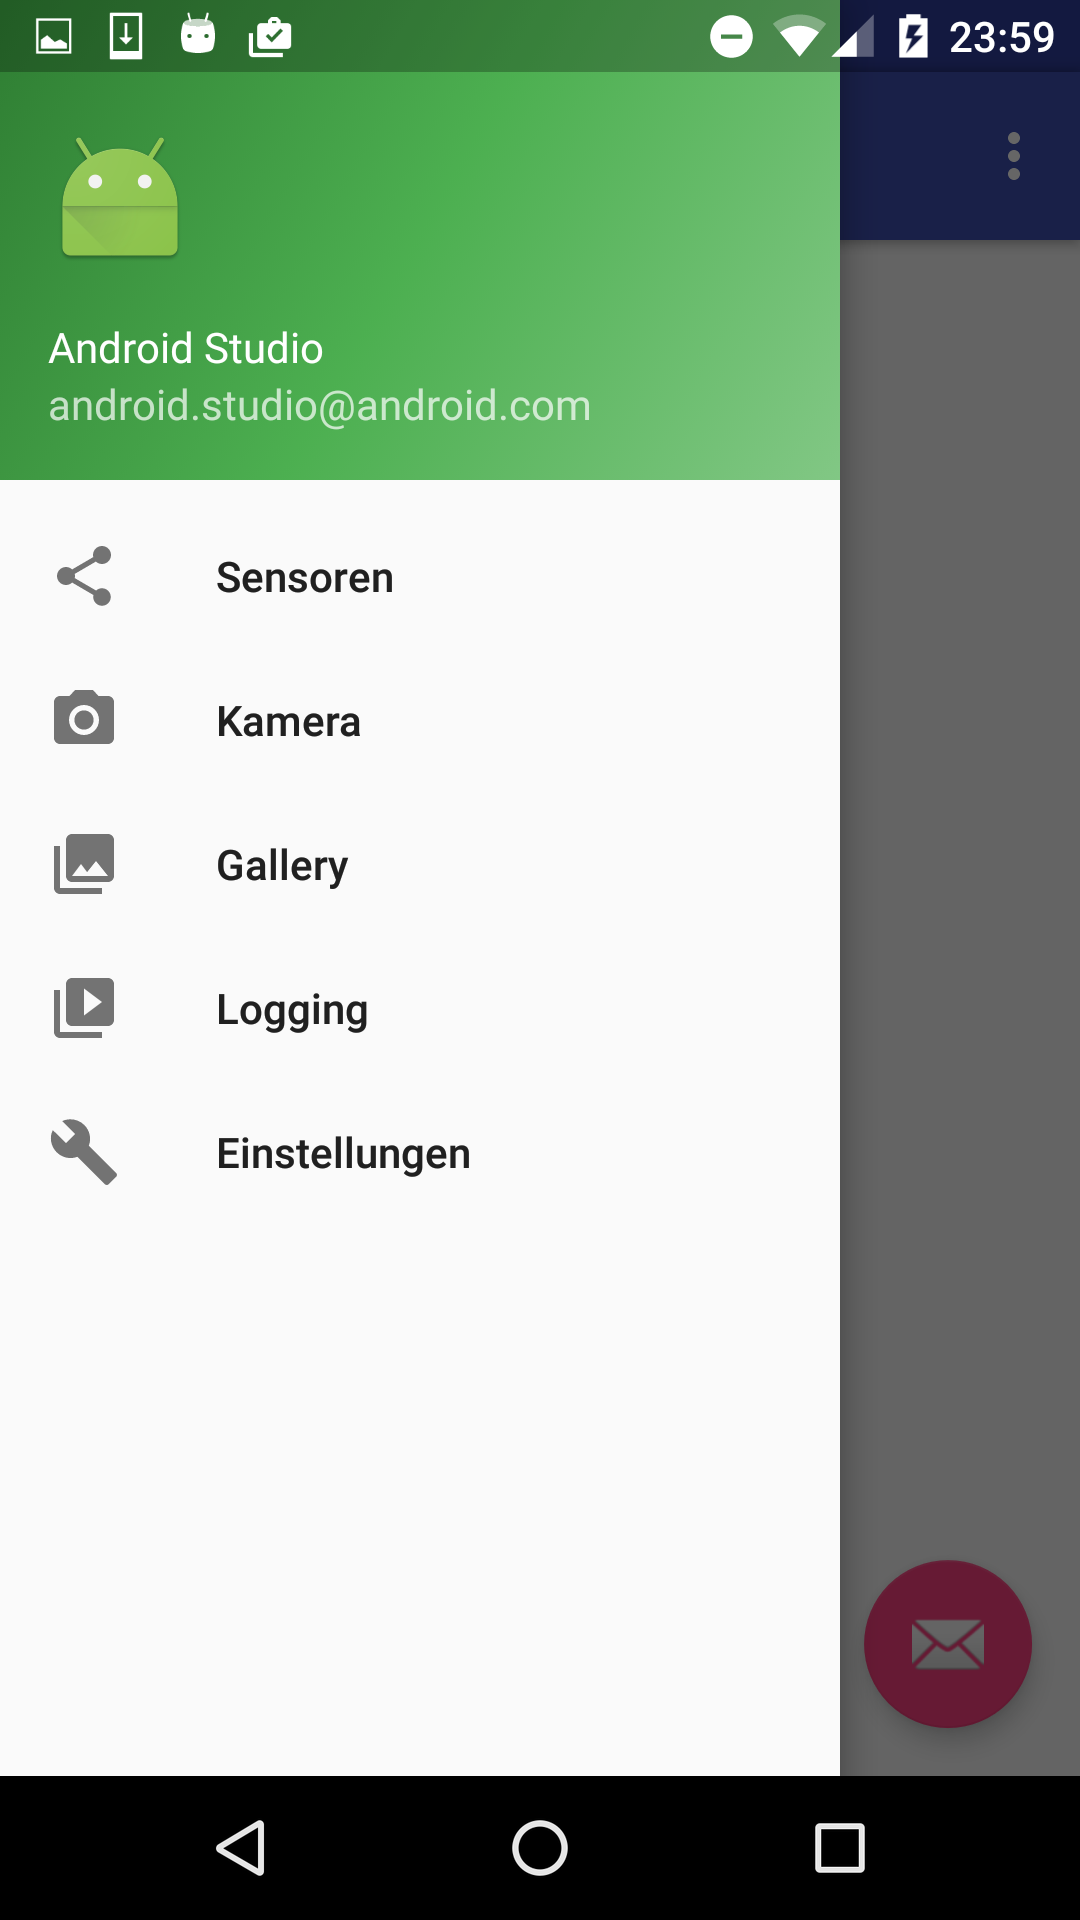
\includegraphics[width=0.4\textwidth]{Bilder/Screenshots/Screenshot_20170214-235908.PNG}
	\caption{Funktionstest-Anwendung: Startseite mit Hauptmenü}
	\label{fig:Main_Menu}
\end{figure}

Wählt der Benutzer im Hauptmenü die Kamerafunktion aus, so wechselt die Anwendung direkt in den Aufnahmemodus. In diesem Modus erscheint das Bild, welches die Kamera aufnimmt im Hintergrund. Vordergründig gibt es einen Auslöse-Button und einen Button für das Wechseln der Kameras im unteren Bildbereich. Ganz oben rechts sind die Blitzfunktionen, durch welche durch klicken navigiert werden kann. 
\\
\\
BILD
\\
\\
In der Galerie (siehe Abbildung \ref{fig:Gallery}) werden dem Benutzer die aufgenommenen und gespeicherten Bilder angezeigt. Durch diese Anzeige kann gescrollt werden. Einzelne Bilder können durch Klicken auf diese ausgewählt werden. Wird ein Bild angeklickt, so bekommt der Benutzer dieses in einem neuen Fenster groß angezeigt. Über den 'Floating Action Button' kann er nun dieses Bild löschen. 

\begin{figure}[h]
	\centering
	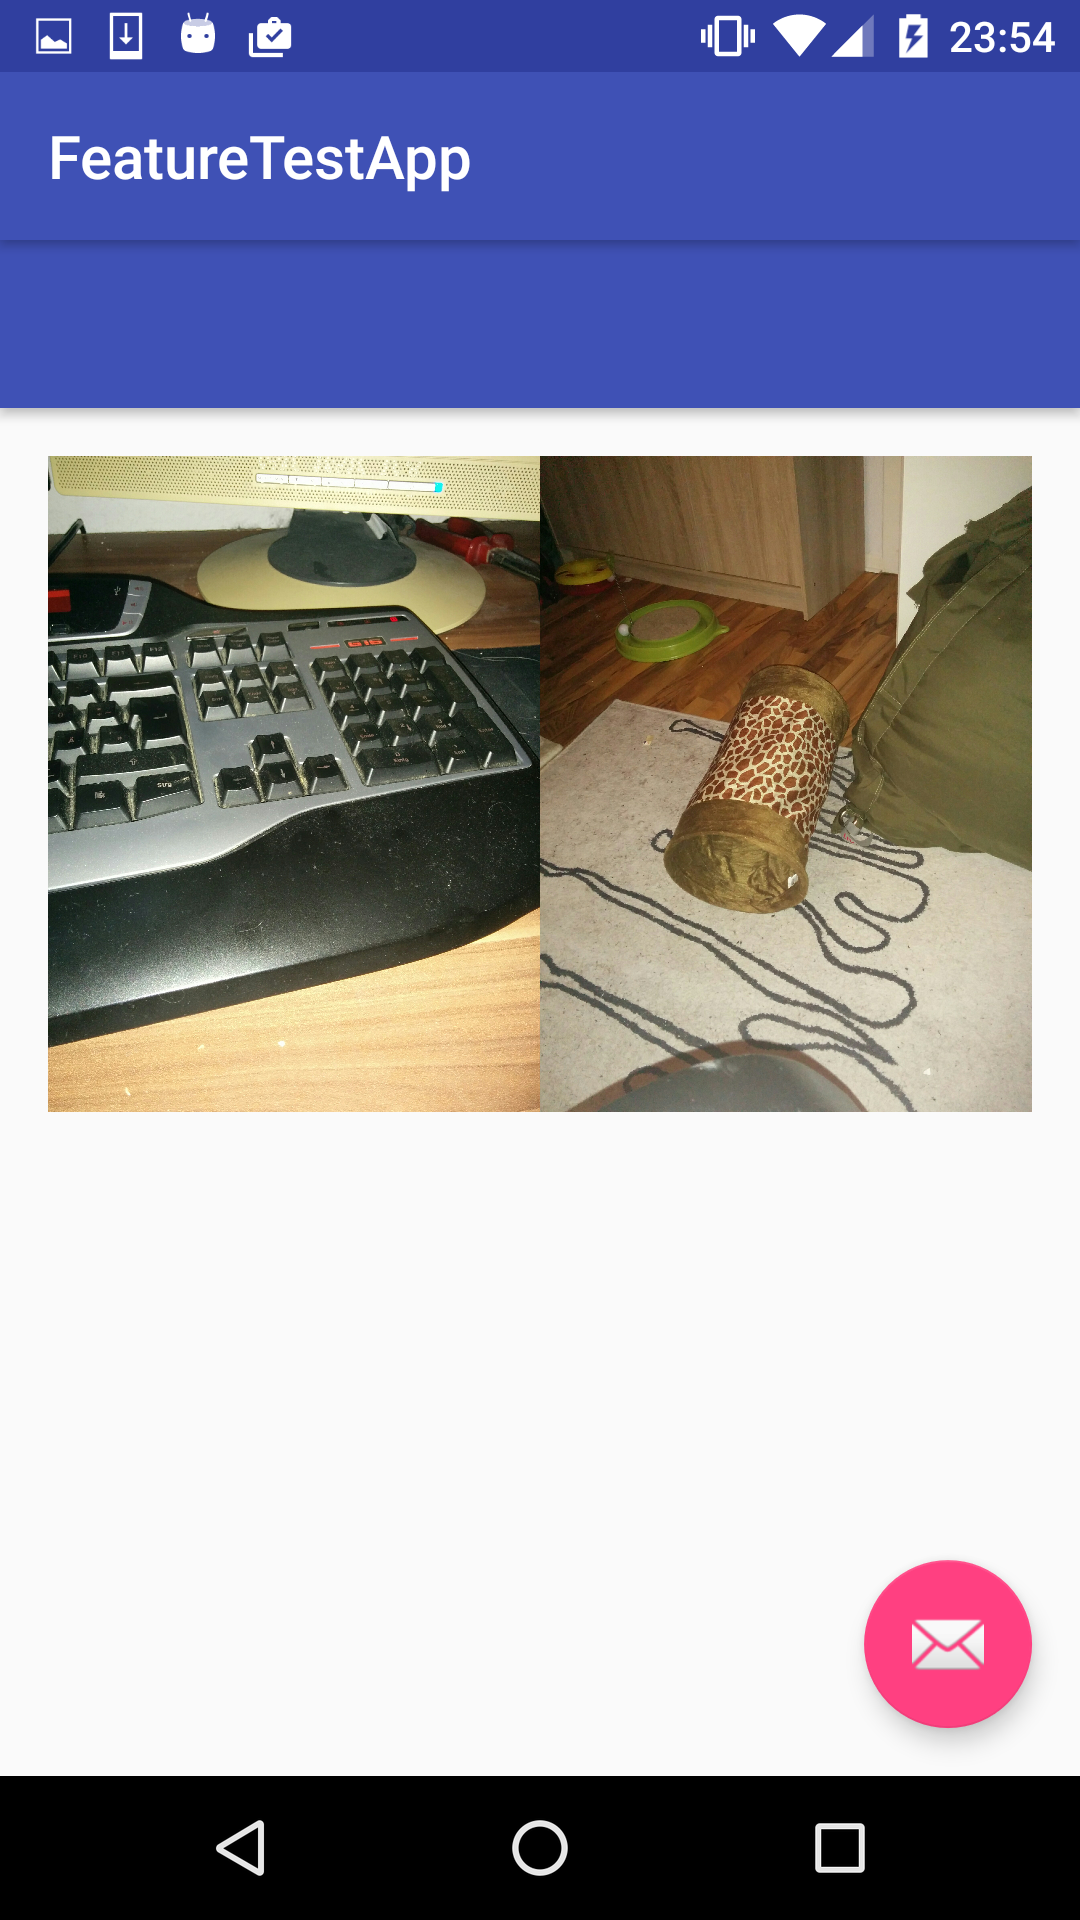
\includegraphics[width=0.4\textwidth]{Bilder/Screenshots/Screenshot_20170214-235454.PNG}
	\caption{Funktionstest-Anwendung: Galerie}
	\label{fig:Gallery}
\end{figure}

Wählt der Benutzer die Standortbestimmung aus, so erscheint im Hintergrund der Seite eine Weltkarte. Ist der Standort vom GPS-Sensor ermittelt worden, so erscheint ein Marker an diesem Ort auf der Weltkarte und die Kartenansicht schwenkt dorthin (siehe Abbildung \ref{fig:GPS}). Der Benutzer hat nun die Möglichkeit weiter in die Karte hinein zu zoomen, um den genauen Standort angezeigt zu bekommen. 
\clearpage

\begin{figure}[h]
	\centering
	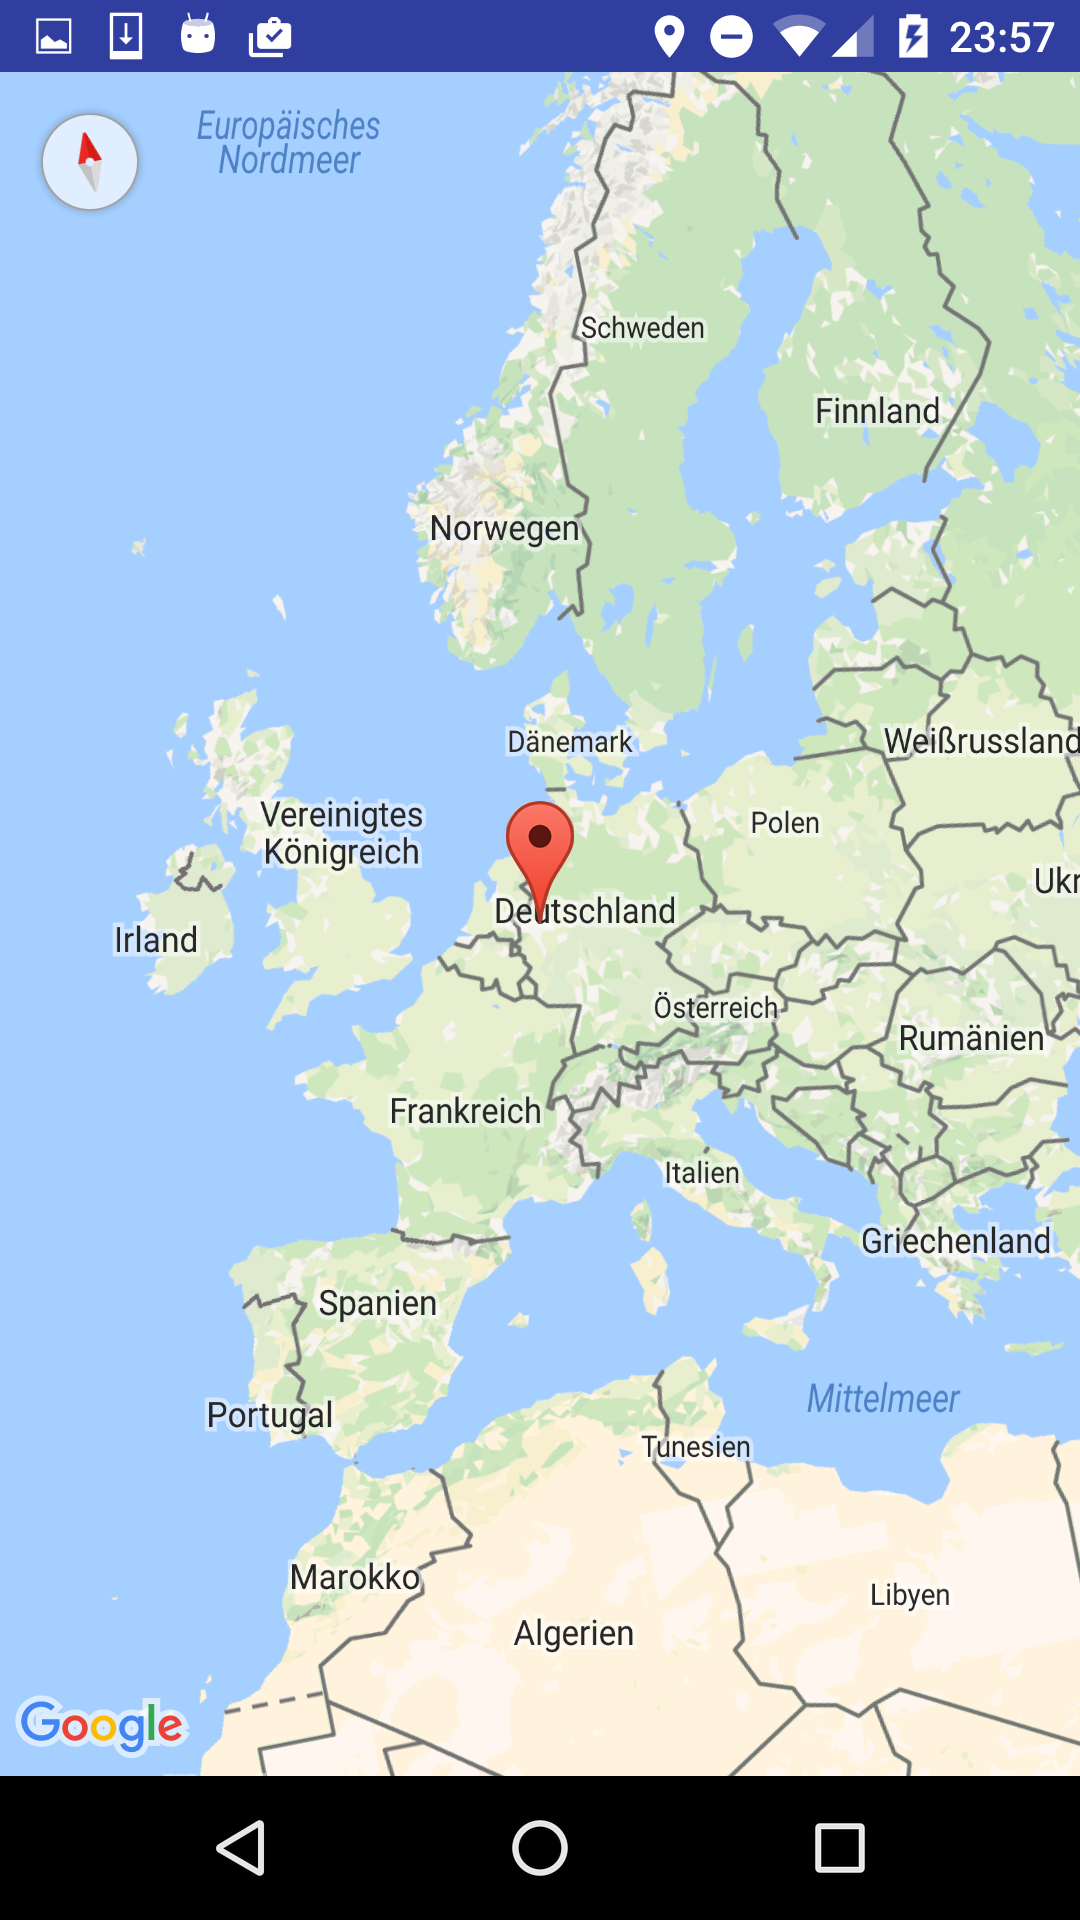
\includegraphics[width=0.4\textwidth]{Bilder/Screenshots/Screenshot_20170214-235726.PNG}
	\caption{Funktionstest-Anwendung: Standortbestimmung}
	\label{fig:GPS}
\end{figure}

Wird die Kompassfunktion gestartet, wird automatisch vom im Smartphone verbauten Magnetometer der magnetische Nordpol ermittelt. Auf der Anzeige wird dem Benutzer eine Kompassrose angezeigt, welche mit der 'N'-Spitze in Richtung magnetischen Nordpol zeigt (siehe Abbildung \ref{fig:Compass}).
\clearpage

\begin{figure}[h]
	\centering
	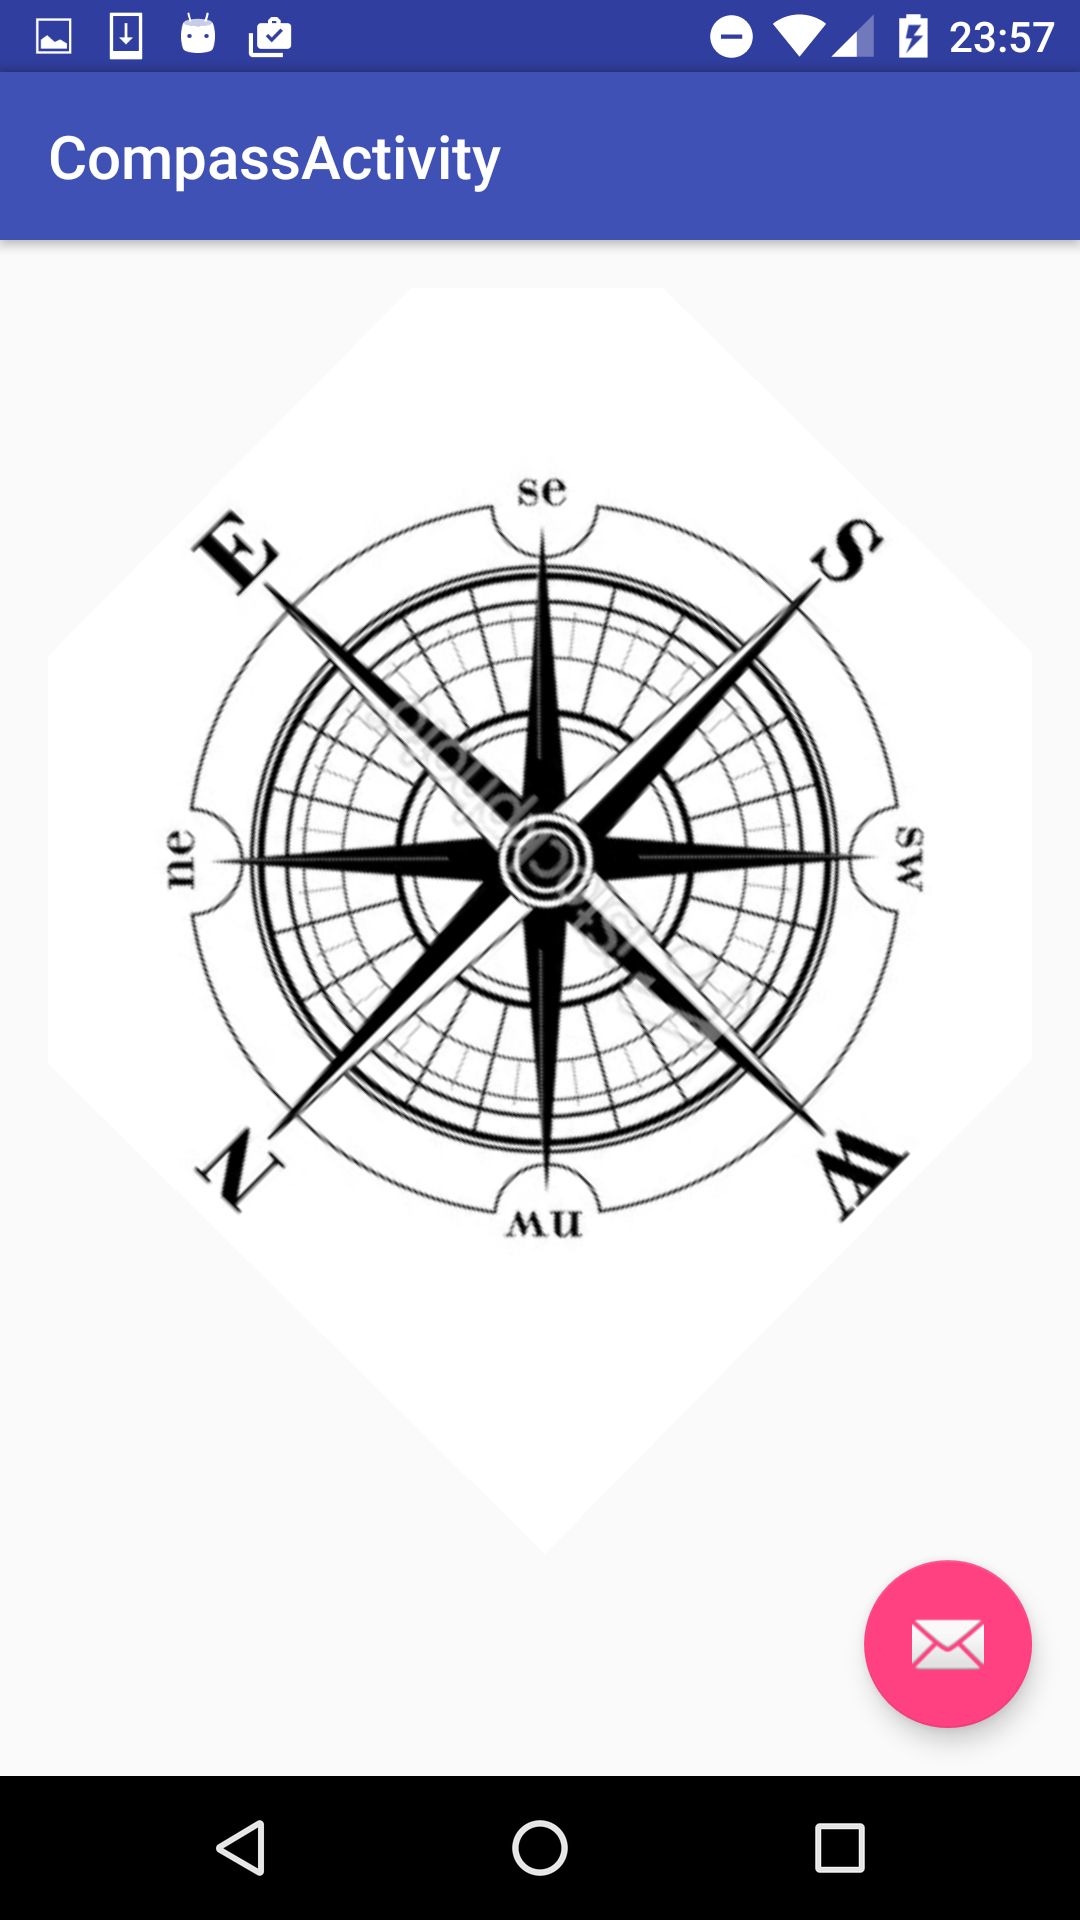
\includegraphics[width=0.4\textwidth]{Bilder/Screenshots/Screenshot_20170214-235753.PNG}
	\caption{Funktionstest-Anwendung: Kompassfunktion}
	\label{fig:Compass}
\end{figure}

Auf der Seite des Bewegungstests werden die vom Beschleunigungssensor ausgelesenen Daten angezeigt. Die Beschleunigungen werden dabei, wie in Kapitel \ref{GrundlagenAccGyro} beschrieben, je Achse angegeben. Zusätzlich zur angezeigten momentanen Beschleunigung werden noch die Werte der maximalen Beschleunigung angezeigt und aktuell gehalten (siehe Abbildung \ref{fig:Accelerometer}). Ein separater Lagesensor wird an dieser Stelle nicht getestet, der Sensortyp 'ORIENTATION' ist veraltet. Anhand des Achsenmodells des Beschleunigungssensors kann die Lage des Smartphones erkannt werden. 
\clearpage

\begin{figure}[h]
	\centering
	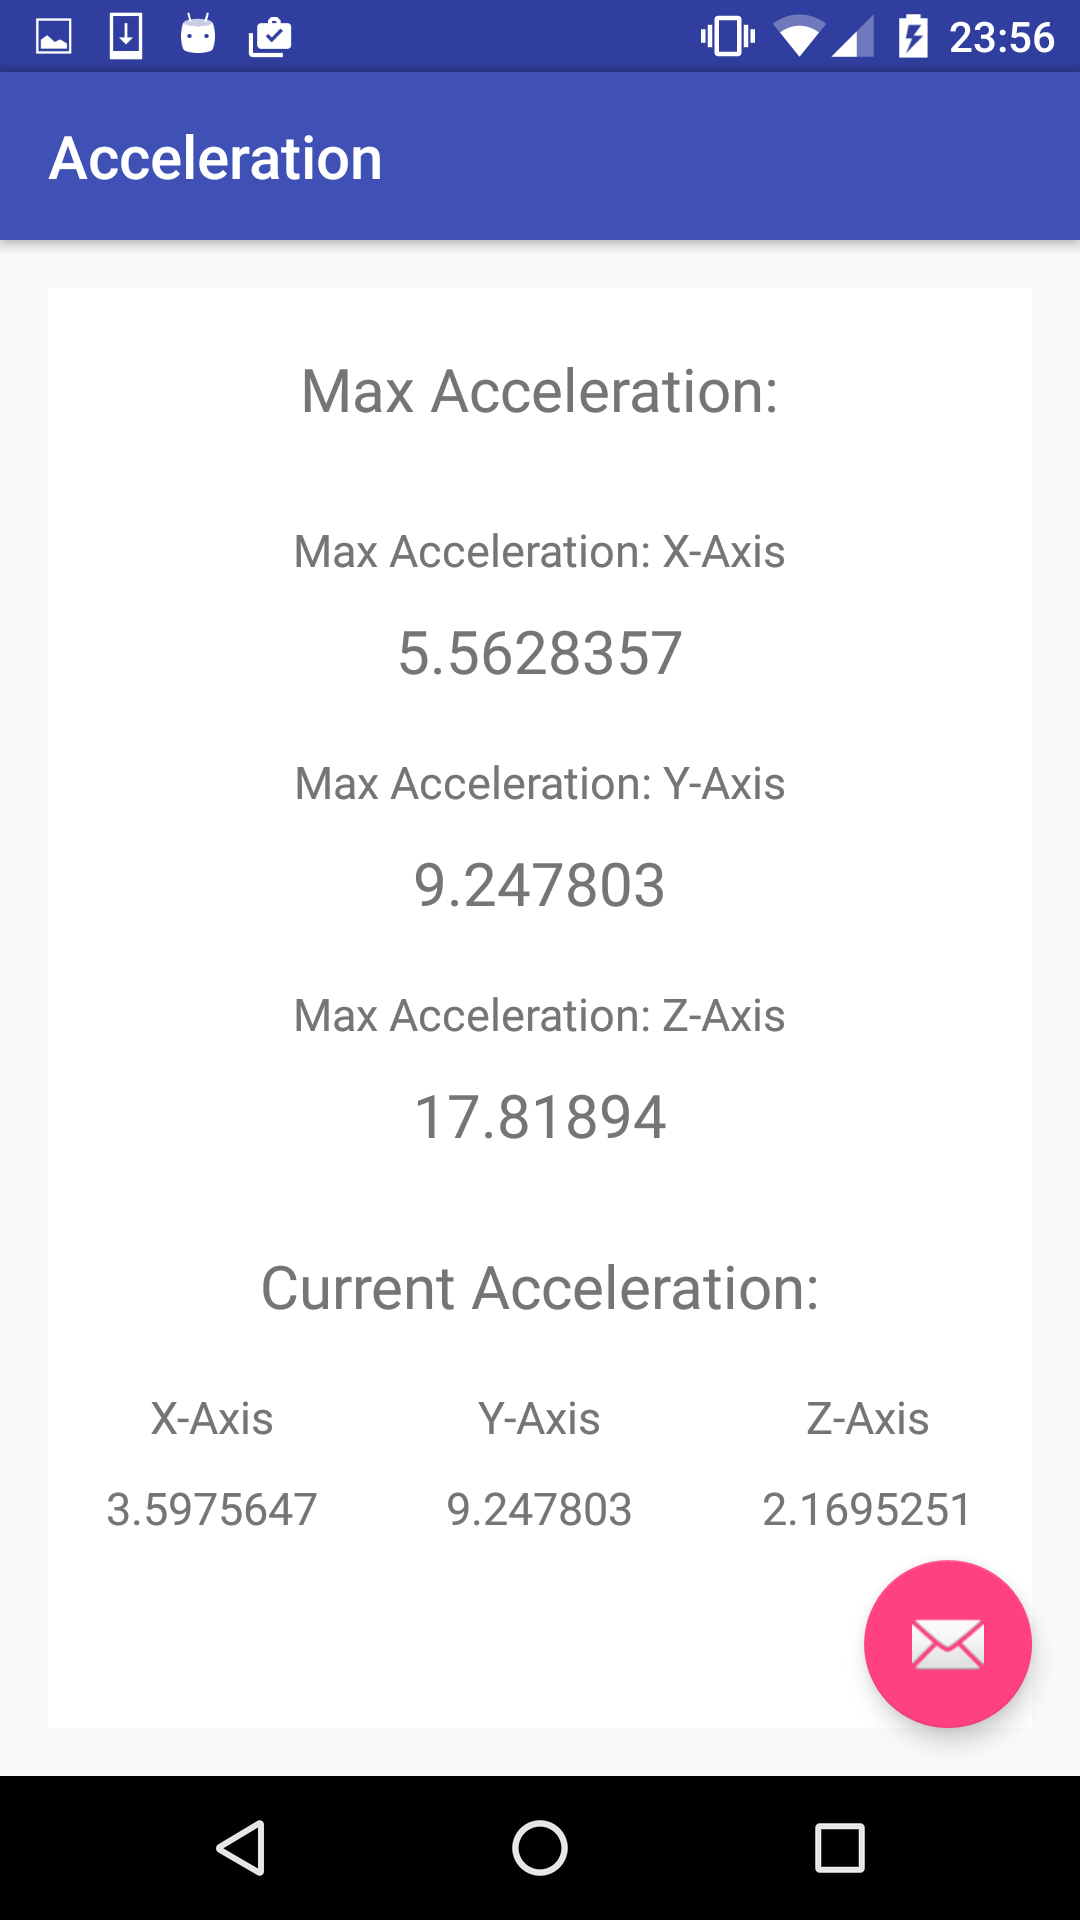
\includegraphics[width=0.4\textwidth]{Bilder/Screenshots/Screenshot_20170214-235635.PNG}
	\caption{Funktionstest-Anwendung: Bewegungstest}
	\label{fig:Accelerometer}
\end{figure}

Bei dem Test des Näherungssensors werden die ausgewerteten Sensordaten an ein 'Toast'-Objekt übergeben. Dieser 'Toast' zeigt 'far' an, wenn sich kein Objekt nahe vor dem Display des Smartphones befindet, und 'near' wenn sich eines genähert hat (siehe Abbildung \ref{fig:Proximity}).

 \clearpage

\begin{figure}[h]
	\centering
	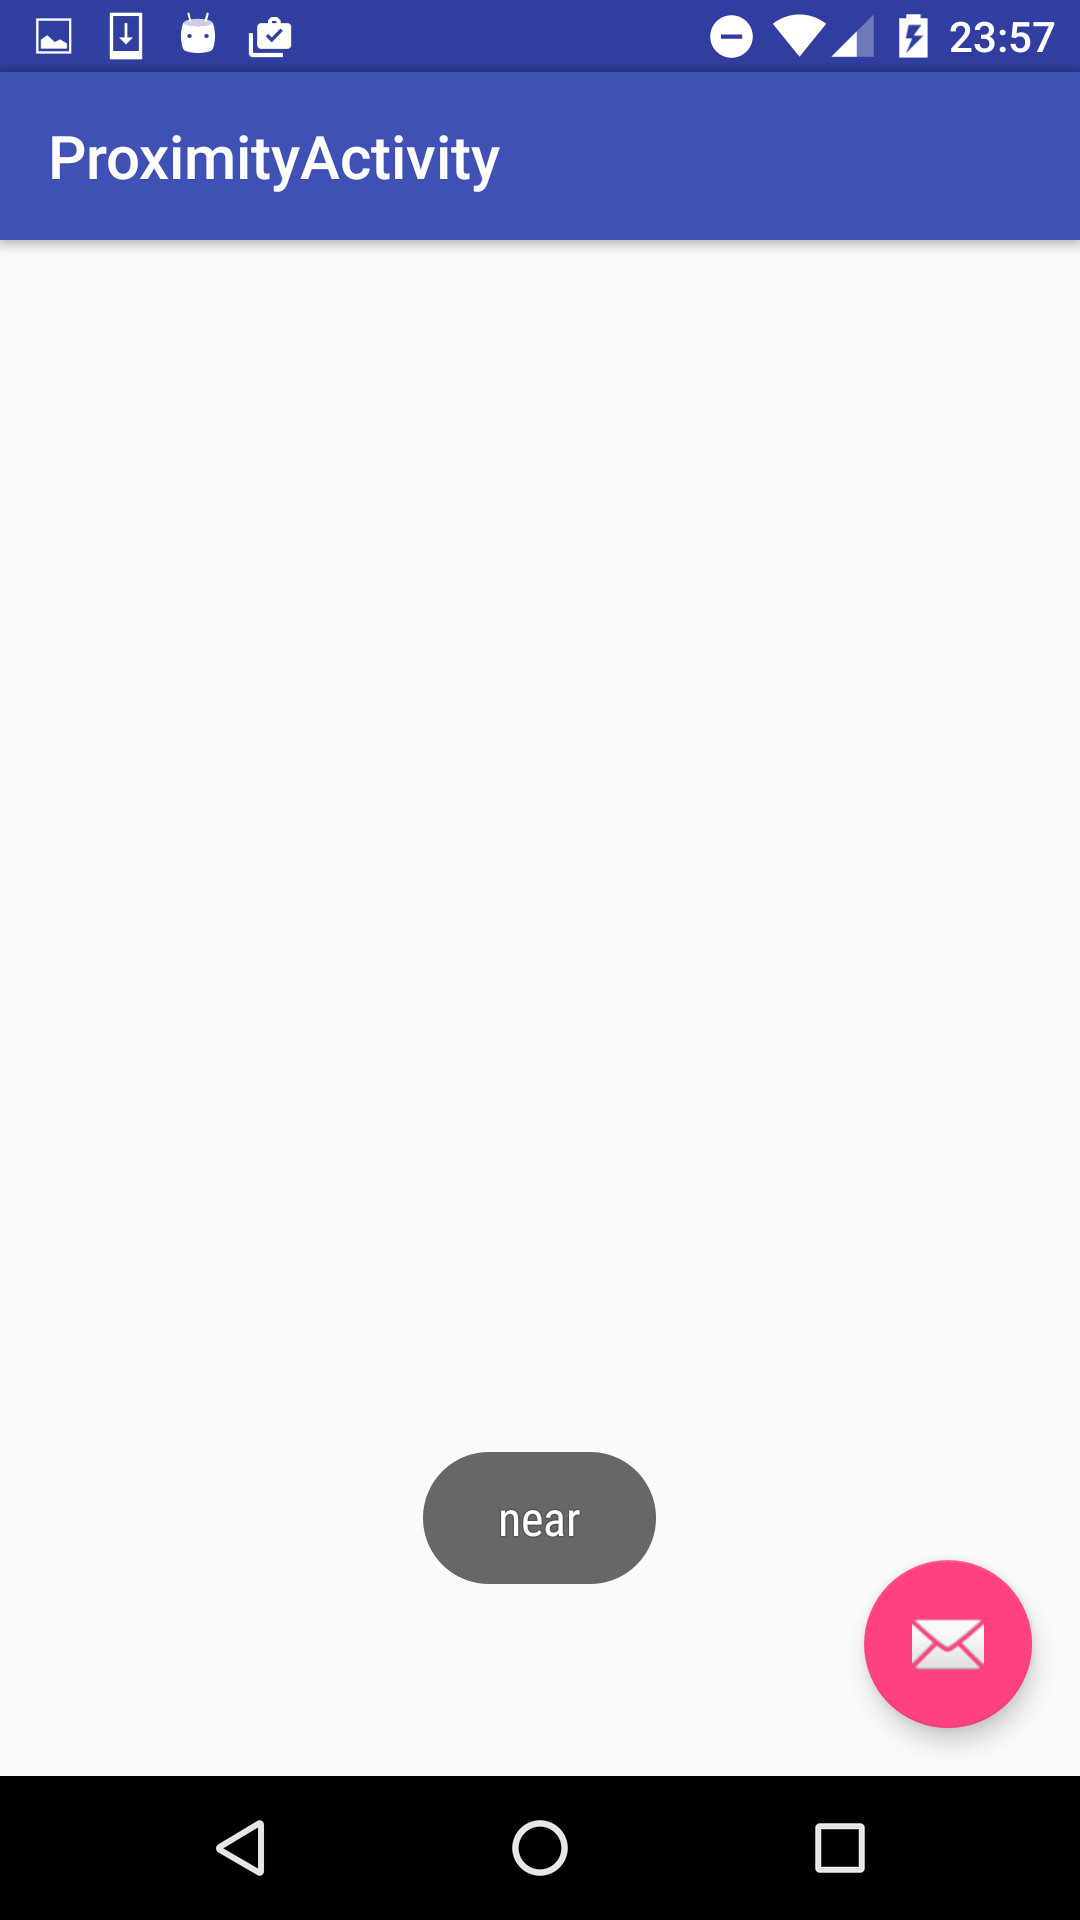
\includegraphics[width=0.4\textwidth]{Bilder/Screenshots/Screenshot_20170214-235744.PNG}
	\caption{Funktionstest-Anwendung: Näherungstest}
	\label{fig:Proximity}
\end{figure}
\chapter{Implementierung}

In diesem Kapitel werden die Implementierungen der Funktionstest-Anwendung ge-mäß der in Kapitel \ref{OOAOOD} erarbeiteten Analyse und Entwurf vorgestellt. Die Anwendung wird insgesamt 4 Mal implementiert: einmal nativ als Referenz und anschließend mit den in Kapitel \ref{Marktanalyse}  vorgestellten 3 Frameworks. Das Hauptaugenmerk liegt hierbei auf den Bereichen, die der Anwendung ein natives Look-And-Feel verleihen sollen. Dies sind entsprechend die Umsetzung der in Kapitel \ref{OOAOODGUI} vorgestellten grafischen Benutzeroberfläche und die Umsetzung der Hardware-Zugriffe für die Nutzung der Sensoren, Kameras und Speicher. So ergeben sich für jede Implementierung 4 Bereiche. Die in Kapitel \ref{OOAOOD} vorgestellten Funktionen der Testanwendung wurden allerdings nicht alle umgesetzt, da auf Mehrfachumsetzung diverser Funktionalitäten, wie zum Beispiel das Laden von Dateien, verzichtet wurde. Solche Mehrfachumsetzungen hätten für die Evaluation keinen Mehrwert ergeben. 

\section{Native Implementierung}

Die native Implementierung der Funktionstest-Anwendung wird mit der IDE 'Android Studio' umgesetzt. Wie schon in Kapitel \ref{AndroidPlattform} beschrieben, ist die Programmiersprache nativer Android Anwendungen Java. Die Anwendung wird gegen die API 23, das bedeutet gegen die Major Version 6 (Marshmallow), kompiliert, da diese Version auch auf dem Testgerät installiert ist. 

\subsection*{Grafische Benutzeroberfläche} \label{natImplGUI}

In Android wird die Struktur der grafischen Benutzeroberfläche über Layouts definiert. Es gibt 2 Wege diese Layouts und ihre Elemente zu deklarieren: Einmal über eine XML-Datei und einmal programmatisch innerhalb der Anwendung über die Nutzung der API. Es wird empfohlen, das Layout über XML-Dateien zu gestalten\footcite{AndroidAPI}, da dies auch eine klarere Trennung der Schicht der grafischen Benutzeroberfläche von der Fachlogikschicht der 3-Schichten-Architektur\footcite{SWTBalzert} begünstigt. 
\\
\\
Für das Hauptmenü und die Auswahl der Sensortests wird, wie in Kapitel \ref{OOAOODGUI} festgelegt wurde, ein 'Navigation Drawer' genutzt. Das Layout dieser Menüs wird in jeweils 3 XML-Dateien beschrieben. Beispielhaft wird an dieser Stelle nur der Code des Hauptmenüs besprochen. Die einzelnen Menüpunkte, die im 'Navigation Drawer' zur Verfügung gestellt werden sollen, werden in der Datei \textit{activity\_main\_drawer.xml} definiert. Wie in unten stehendem Listing \ref{lst:DrawerMenu} dargestellt, wird pro Eintrag im Drawer-Menü ein Item-Objekt definiert. Diesen Item-Objekten werden jeweils eine eindeutige ID, ein Icon und eine Bezeichnung, welche dann im Menü angezeigt wird, übergeben. 

\begin{lstlisting}[caption=Definition der Menüpunkte im 'Navigation Drawer' der Hauptseite in der Datei \textit{activity\_main\_drawer.xml}, label=lst:DrawerMenu, language=XML]
<group android:checkableBehavior="single">      
		...              
        <item
            android:id="@+id/nav_camera"
            android:icon="@drawable/ic_menu_camera"
            android:title="Kamera" />
        <item
            android:id="@+id/nav_gallery"
            android:icon="@drawable/ic_menu_gallery"
            android:title="Gallery" />       
		...               
    </group>
\end{lstlisting} 

Jeder 'Navigation Drawer' hat einen Header. Das Design und der Aufbau dessen wird in der Datei \textit{nav\_header\_main.xml} definiert (siehe Listing \ref{lst:DrawerHeader}). Hier wird bei der Funktionstest-Anwendung der Default-Header von Android Studio genutzt. Für den farbigen Hintergrund, sowie das Android-Icon werden Vorlagen im \textit{drawable}-Ordner mitgeliefert. Diese werden in der Layout-Datei referenziert, wie in Zeile 4 und 11 im unten stehenden Listing \ref{lst:DrawerHeader} zu sehen ist.
\clearpage

\begin{lstlisting}[caption=Definition des Headers des 'Navigation Drawers' in der Datei \textit{nav\_header\_main.xml}, label=lst:DrawerHeader, language=XML]
<LinearLayout xmlns:android="http://schemas.android.com/apk/res/android"
    android:layout_width="match_parent"
    android:layout_height="@dimen/nav_header_height"
    android:background="@drawable/side_nav_bar"    
    ...
    <ImageView
        android:id="@+id/imageView"
        android:layout_width="wrap_content"
        android:layout_height="wrap_content"
        android:paddingTop="@dimen/nav_header_vertical_spacing"
        android:src="@android:drawable/sym_def_app_icon" />

    <TextView
        android:layout_width="match_parent"
        android:layout_height="wrap_content"
        android:paddingTop="@dimen/nav_header_vertical_spacing"
        android:text="Android Studio"
        android:textAppearance="@style/TextAppearance.AppCompat.Body1" />
    ...
</LinearLayout>
\end{lstlisting} 

Das Layout und der Inhalt des 'Navigation Drawers' werden nun in der Layout-Datei des Hauptmenüs, der \textit{MainActivity} referenziert (siehe Listing \ref{lst:MainMenu} Zeile 13 und 14). Hier wird noch über \textit{include} die \textit{App Bar}, die am oberen Bildrand positioniert ist, importiert (siehe Listing \ref{lst:MainMenu} Zeile 2 bis 5). Das \textit{App Bar} Design, welches in der Datei \textit{app\_bar\_main.xml} definiert ist, bringt noch einen \textit{FloatingActionButton} mit sich, der unten rechts im Bildschirm positioniert wird. 

\begin{lstlisting}[caption=Layout des Hauptmenüs in der Datei \textit{activity\_main.xml}, label=lst:MainMenu, language=XML]
...
<include
        layout="@layout/app_bar_main"
        android:layout_width="match_parent"
        android:layout_height="match_parent" />

    <android.support.design.widget.NavigationView
        android:id="@+id/nav_view"
        android:layout_width="wrap_content"
        android:layout_height="match_parent"
        android:layout_gravity="start"
        android:fitsSystemWindows="true"
        app:headerLayout="@layout/nav_header_main"
        app:menu="@menu/activity_main_drawer" />
...
\end{lstlisting} 

Für die Kamerafunktion musste keine eigene Benutzeroberfläche gestaltet werden, da über die API die in Android integrierte Kameraanwendung direkt angesprochen und gestartet wird. Diese Anwendung stellt entsprechend der Anforderungen aus Kapitel \ref{Anforderungsanalyse} sämtliche Benutzereingabemöglichkeiten bezüglich Kamerawechsel oder Blitzeinstellungen zur Verfügung. 
\\
\\
Für die Darstellung der Werte des Beschleunigungssensors wurden \textit{LinearLayout}-Objekte in 3 Ebenen verwendet, welche mit \textit{TextView}-Objekten gefüllt sind, über die die Werte dem Benutzer präsentiert werden. Zur allgemeinen Aufteilung der Layout-Elementen lässt sich sagen, dass die globalen Elemente einer Seite, wie die \textit{AppBar} oder der \textit{FloatingActionButton} in der hierarchisch obersten Layout-Datei \textit{activity\_[name].xml} definiert werden.

\subsection*{Sensoren} \label{ImplNativSensors}

Da die Zugriffe auf die Sensoren und das Auslesen ihrer Daten äquivalent sind werden diese Vorgänge hier am Beispiel des Näherungssensors erläutert. Damit Die \textit{Activity} auf Sensordaten zugreifen kann, braucht sie ein \textit{SensorManager}-Objekt und ein \textit{Sensor}-Objekt (siehe Listing \ref{lst:SensorInit}).

\begin{lstlisting}[caption=Definition und Initialisierung von Sensor und SensorManager, label=lst:SensorInit, language=Java]
private SensorManager mSensorManager;
private Sensor mSensor;
...
mSensorManager = (SensorManager) getSystemService(SENSOR_SERVICE);
mSensor = mSensorManager.getDefaultSensor(Sensor.TYPE_PROXIMITY);
\end{lstlisting} 

Beide Objekte werden direkt beim initialen Start der \textit{Activity} erzeugt. Der \textit{SensorManager} wird benötigt um die \textit{Listener}, welche auf den Sensor horchen, zu registrieren und abzumelden. Dies geschieht in den Methoden \textit{onResume()} und \textit{onPause()} (siehe Listing \ref{lst:onResumeOnPause}). 
\clearpage

\begin{lstlisting}[caption=Die Methoden \textit{onResume()} und \textit{onPause()}, label=lst:onResumeOnPause, language=Java]
protected void onResume() {
        super.onResume();
        mSensorManager.registerListener(this, mSensor,
                SensorManager.SENSOR_DELAY_NORMAL);
}
protected void onPause() {
        super.onPause();
        mSensorManager.unregisterListener(this);
}
\end{lstlisting} 

Die vom Sensor übermittelten Daten werden in einem \textit{SensorEvent}-Objekt der Methode \textit{onSensorChanged()} übergeben. Dort können diese Daten weiterverarbeitet werden. Für die Verarbeitung der Daten des Näherungssensors bedeutet dies, dass dort die Textausgaben 'near' und 'far' generiert werden (siehe Listing \ref{lst:SensorChanged}). 

\begin{lstlisting}[caption=Die Methode \textit{onSensorChanged()}, label=lst:SensorChanged, language=Java]
public void onSensorChanged(SensorEvent event) {
        if (event.values[0] == 0) {
            Toast.makeText(getApplicationContext(), "near", Toast.LENGTH_SHORT).show();
        } else {
            Toast.makeText(getApplicationContext(), "far", Toast.LENGTH_SHORT).show();
        }
}
\end{lstlisting} 

Für den Zugriff auf manche Sensoren und Dienste benötigt die Anwendung eine besondere Erlaubnis. Diese Erlaubnis wird der Anwendung im \textit{AndroidManifest} gegeben. Reicht dies nicht aus, muss eine Anfrage an den Benutzer gestellt werden, welcher dann mit seiner Zustimmung die Erlaubnis erteilt. Im \textit{AndroidManifest} wird diese Erlaubnis über den \textit{uses-permission}-Parameter eingetragen (siehe Listing \ref{lst:usesPermission}).

\begin{lstlisting}[caption=Erlaubnis für die Nutzung eines Dienstes im \textit{AndroidManifest}, label=lst:usesPermission, language=XML]
<uses-permission android:name="android.permission.ACCESS_FINE_LOCATION" />
\end{lstlisting}  

Die Anfrage einer Erlaubnis direkt an den Benutzer wird im Code der jeweiligen \textit{Activity} realisiert, wie in Listing \ref{lst:requestPermission} zu sehen ist:
\clearpage

\begin{lstlisting}[caption=Generierung der Anfrage für die Erlaubnis einen Dienst zu nutzen an den Benutzer, label=lst:requestPermission, language=Java]
...
if (ContextCompat.checkSelfPermission(this, android.Manifest.permission.ACCESS_FINE_LOCATION) != PackageManager.PERMISSION_GRANTED) {
            ActivityCompat.requestPermissions(this,
                    new String[]{android.Manifest.permission.ACCESS_FINE_LOCATION},
                    MY_PERMISSIONS_REQUEST_ACCESS_FINE_LOCATION);
        }
...
\end{lstlisting} 

\subsection*{Kameras}

Wie bereits in Kapitel \ref{natImplGUI} erwähnt, wird für die Kameranutzung die interne Kameraanwendung von Android aufgerufen. Dies geschieht direkt, nachdem vom Hauptmenü aus die Kamerafunktion (\textit{CameraActivity}) aufgerufen wird, also in der \textit{onCreate()}-Methode der \textit{CameraActivity}. Hier ist dieser Aufruf, wie in Listing \ref{lst:callTakeAPic} zu sehen ist in der Methode \textit{takeAPicture()} gekapselt:

\begin{lstlisting}[caption=Aufruf der Android-Kamerafunktion in der \textit{onCreate()}-Methode der Klasse \textit{CameraActivity}, label=lst:callTakeAPic, language=Java]
@Override
    protected void onCreate(Bundle savedInstanceState) {
        super.onCreate(savedInstanceState);
        setContentView(R.layout.activity_camera);

        //dispatchTakePictureIntent();
        _imageView = (ImageView) findViewById(R.id.imageView1);
        takeAPicture();
    }
\end{lstlisting}  

Eine \textit{Activity} wird in Android über einen \textit{Intent} aufgerufen. Ein \textit{Intent} kann auf verschiedene Weisen erzeugt werden. In diesem Fall übergeben wir dem Konstruktor eine \textit{Action} in Form einer \textbf{String}-Variable, nämlich die \textit{ACTION\_IMAGE\_CAPTURE} (siehe Listing \ref{lst:IntentCamera}).
\clearpage

\begin{lstlisting}[caption=Methode \textit{takeAPicture()}: Aufruf der Android-Kamerafunktion über einen \textit{Intent}, label=lst:IntentCamera, language=Java]
private void takeAPicture() {
        Intent intent = new Intent(MediaStore.ACTION_IMAGE_CAPTURE);
        try {
            _file = createImageFile();
        } catch (IOException e) {
            // ToDo
        }
        intent.putExtra(MediaStore.EXTRA_OUTPUT, Uri.fromFile(_file));
        startActivityForResult(intent, REQUEST_IMAGE_CAPTURE);
    }
\end{lstlisting}  

Die Methode \textit{createImageFile()}, welche oben im Listing \ref{lst:IntentCamera} in Zeile 4 aufgerufen wird, generiert Namen für die Bilder, die mit der Kamerafunktion aufgenommen und gespeichert werden. Sollen noch weitere Funktionen ausgeführt werden, sobald ein Bild gespeichert wird, so müssen diese in der Methode \textit{onActivityResult()} definiert werden. Diese Methode wird automatisch immer dann ausgeführt, wenn der Benutzer ein Bild abspeichert. Als Beispiel können hier noch Bildbearbeitungen, wie Formatänderungen, vorgenommen werden, oder das Bild kann, wie Listing \ref{lst:AndroidGallery} zeigt, in der Android \textit{Gallery} zur Verfügung gestellt werden.

\begin{lstlisting}[caption=Bereitstellen des gespeicherten Bildes für die Android \textit{Gallery}, label=lst:AndroidGallery, language=Java]
...
Intent mediaScanIntent = new Intent(Intent.ACTION_MEDIA_SCANNER_SCAN_FILE);
Uri contentUri = Uri.fromFile(this._file);
mediaScanIntent.setData(contentUri);
this.sendBroadcast(mediaScanIntent);
...
\end{lstlisting}  

\subsection*{Speicherzugriffe}

Der in Kapitel \ref{PlanungAnwSpeicher} beschriebene 'External Storage' wird über die Methode \textit{getExternalFilesDir()} andressiert. Da wir in diesem Fall dort Bilder speichern wollen, übergeben wir der Methode dies als Information in Form von \textit{Environment.DIRECTORY\_PICTURES}. In diesem Ordner wird nun der Ordner 'Feature\_Test\_App' erzeugt, wie in Listing \ref{lst:SpeicherZugriff} zu sehen ist.
\clearpage

\begin{lstlisting}[caption=Adressieren des 'External Storage' und Anlegen eines Ordners für die Fotos der Funktionstest-Anwendung, label=lst:SpeicherZugriff, language=Java]
public void CreateDirectoryForPictures() {
        File pubPictures = getExternalFilesDir(Environment.DIRECTORY_PICTURES);
        //this._dir = new File(Environment.getExternalStoragePublicDirectory(Environment.DIRECTORY_PICTURES), "FeatureTestApp");
        CameraActivity._dir = new File(pubPictures, "Feature_Test_App");
        if (!CameraActivity._dir.exists())
        {
            CameraActivity._dir.mkdirs();
        }
    }
\end{lstlisting}

\section{Implementierung mit Xamarin}

Für die Entwicklung von Xamarin Anwendungen auf einem Windows PC wird die IDE 'Visual Studio' verwendet. Die verwendete Programmiersprache ist, wie schon in Kapitel \ref{chpXamarin} erwähnt, C\#. Für den optimalen Vergleich zur nativen Anwendung wird auch die Xamarin-Version gegen die API 23, das bedeutet gegen die Major Version 6 (Marshmallow), kompiliert. 

\subsection*{Grafische Benutzeroberfläche}

Wenn man sich dafür entscheidet in Xamarin eine Anwendung für Android mit den bekannten Android-Bedienelementen zu schreiben, anstelle einer Anwendung mit Xamarin.Forms, so ergibt sich die gleiche Dateistruktur im Projekt wie auch bei der nativen Anwendung. Die Layout-Dateien enden allerdings hier nicht auf .xml, sondern auf .axml. Der interne Aufbau der Layout-Dateien ist identisch mit dem der nativen Layout-Dateien. Möchte man also eine native Anwendung in Xamarin migrieren, ließe sich das Layout ganz einfach übernehmen. 
\\
\\
Um unnötigen doppelten Code auszusparen, wurde ab dieser Implementierung nur noch mit einem \textit{Navigation Drawer} gearbeitet, anstelle von zwei. Da die Inhalte der Layout-Dateien des \textit{Drawers}, wie oben schon erwähnt, identisch mit der nativen Version sind, wird an dieser Stelle auf Ausschnitte dieser verzichtet. Der Zuordnung der einzelnen Seiten der Anwendung zu den Navigationselementen erfolgt ebenfalls ähnlich der nativen Version über \textit{Intents}. Der Code ist bei der Xamarin-Anwendung zwar in C\# geschrieben, die aufgerufene Klasse \textit{Intent} stammt dabei aus dem Android SDK (siehe Listing \ref{lst:ZuordnungNavigationselemente}). 

\begin{lstlisting}[caption=Zuweisung der einzelnen Seiten der Anwendung zu den Navigationselementen im Navigation Drawer, label=lst:ZuordnungNavigationselemente, language=Java]
void NavigationView_NavigationItemSelected(object sender, NavigationView.NavigationItemSelectedEventArgs e)
        {
            switch (e.MenuItem.ItemId)
            {
                case (Resource.Id.nav_camera):
                    Intent intentCamera = new Intent(this, typeof(CameraActivity));
                    StartActivity(intentCamera);
                    break;
                case (Resource.Id.nav_gallery):
                    Intent intentGallery = new Intent(this, typeof(PictureGalleryActivity));
                    StartActivity(intentGallery);
                    break;
                    
                    ...
            }
        }
\end{lstlisting}


In nachfolgender Abbildung \ref{fig:MenuXamarin} ist der \textit{NavigationDrawer} mit den einzelnen Menüpunkten abgebildet. Wie bei der nativen Anwendung ist der \textit{NavigationDrawer} auch in der Xamarin-Anwendung über Wischen und über den Hamburger-Button oben links in der Appbar aus- und wieder einklappbar.
\clearpage

\begin{figure}[h]
	\centering
	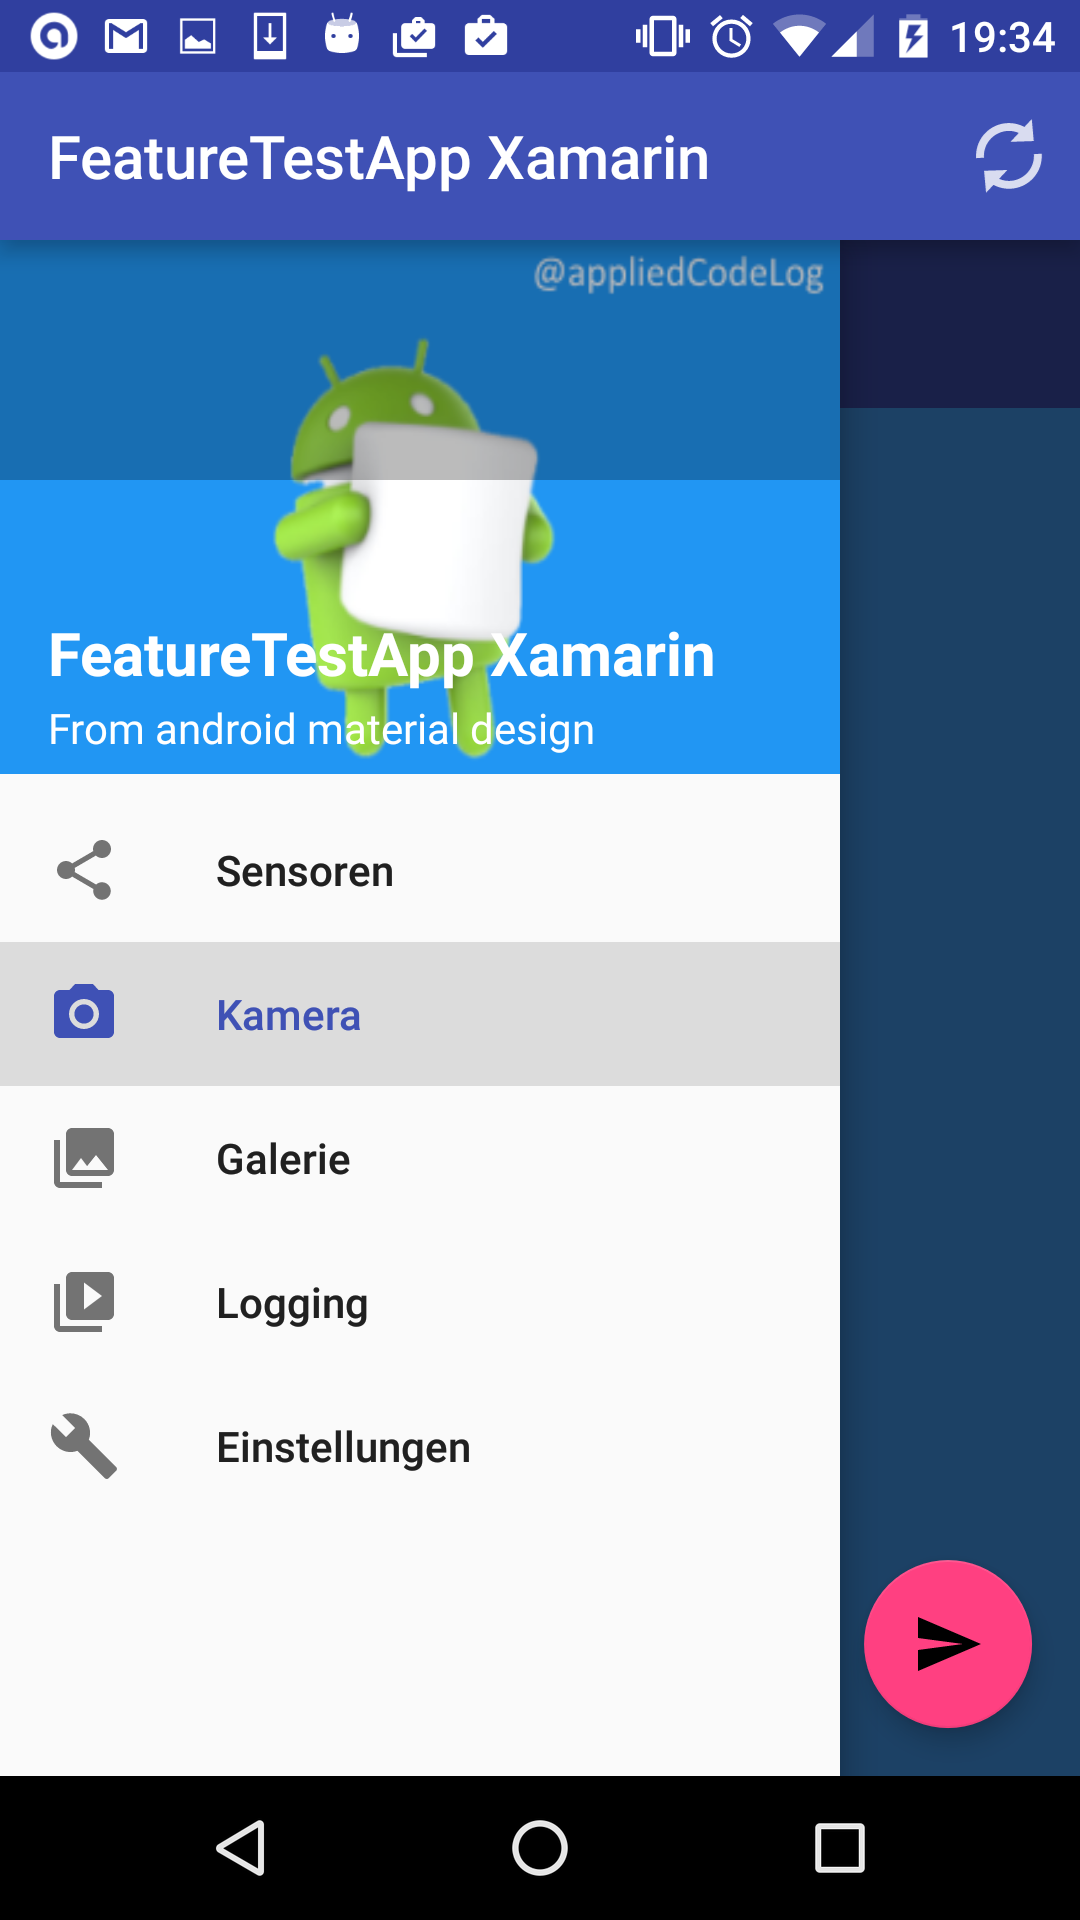
\includegraphics[width=0.4\textwidth]{Bilder/Screenshot_20170328-193448.PNG}
	\caption{Menü in der Xamarin Anwendung}
	\label{fig:MenuXamarin}
\end{figure}

In der Xamarin-Anwendung wird wie in der nativen Anwendung auf der Seite mit der Kamerafunktionalität über die API die in Android integrierte Kameraanwendung direkt angesprochen und gestartet. So verfügt die Anwendung auch über die Möglichkeit des Kamerawechsels und des Einstellen des Blitzes. 
\\
\\
Der \textit{FloatingActionButton} wird wie auch die anderen GUI-Elemente wie der \textit{NavigationDrawer} in einer Layout-Datei deklariert. Da der \textit{FloatingActionButton} auf allen Seiten zur Verfügung stehen soll, wird er wie in der nativen Anwendung in der Layout-Datei \textit{app\_bar.axml} deklariert, welche dann in der Haupt-Layout-Datei importiert wird. Die Deklaration des \textit{FloatingActionButton} ist unten im Listing \ref{lst:FABXamarin} dargestellt. Bei der Deklaration können Farbe, Größe und Positionierung mit angegeben werden. Wie in Kapitel \ref{PlanungAnwGUI} dargestellt, wird in dieser Anwendung der \textit{FloatingActionButton} rechts unten positioniert, was über die Angabe 'bottom|right' geschieht (siehe Listing \ref{lst:FABXamarin}). 
\clearpage

\begin{lstlisting}[caption=Deklaration des \textit{FloatingActionButton} in der Datei \textit{app\_bar.axml}, label=lst:FABXamarin, language=Java]
...
<com.refractored.fab.FloatingActionButton
            android:id="@+id/fab"
            android:layout_width="wrap_content"
            android:layout_height="wrap_content"
            android:layout_gravity="bottom|right"
            android:layout_margin="16dp"
            android:src="@drawable/ic_action_content_new"
            fab:fab_colorNormal="@color/primary"
            fab:fab_colorPressed="@color/primary_pressed"
            fab:fab_colorRipple="@color/ripple" />
...
\end{lstlisting}

\subsection*{Sensoren}

Wie auch bei der nativen Anwendung müssen Berechtigungen im \textit{AndroidManifest} erteilt werden. Hierfür bietet Xamarin in Visual Studio eine grafische Benutzeroberfläche, in der die benötigten Berechtigungen einfach ausgewählt werden können und anschließend automatisch in die Datei \textit{AndroidManifest.xml} eingetragen werden (siehe Abbildung \ref{fig:PermissionsAuswXamarin}). 

\begin{figure}[h]
	\centering
	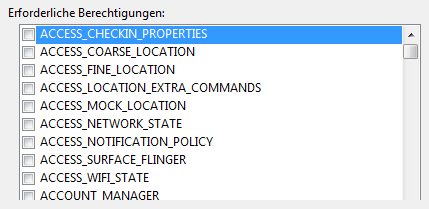
\includegraphics[width=0.7\textwidth]{Bilder/Permissions_Xamarin.PNG}
	\caption{Auswahlfenster für benötigte Berechtigungen in Xamarin (Visual Studio)}
	\label{fig:PermissionsAuswXamarin}
\end{figure}

Der generierte Eintrag in das \textit{AndroidManifest} ist nachfolgend in Listing \ref{lst:usesPermissionXamarin} dargestellt:

\begin{lstlisting}[caption=Erlaubnis für die Nutzung eines Dienstes im \textit{AndroidManifest} (Xamarin), label=lst:usesPermissionXamarin, language=XML]
<uses-permission android:name="android.permission.ACCESS_FINE_LOCATION" />
\end{lstlisting}

Auch das Auslesen von Sensordaten ist nahezu identisch mit der nativen Variante. Für eine gute Vergleichbarkeit bleiben wir auch in diesem Kapitel bei der Vorstellung der Nutzung des Näherungssensors. Wie man in unten stehendem Listing \ref{lst:ProximityXamarin} erkennen kann, ist der Code zum Auslesen der Daten des Näherungssensors praktisch identisch mit dem aus Listing \ref{lst:SensorChanged} (nativ). Auch hier wird die Bearbeitung der Daten in der Methode \textit{onSensorChanged()} der Klasse \textit{SensorEventListener} vorgenommen.

\begin{lstlisting}[caption=Auslesen der Daten des Näherungssensors (Xamarin), label=lst:ProximityXamarin, language=Java]
public void onSensorChanged(SensorEvent event) {
        if (event.values[0] == 0) {
            Toast.MakeText(this, "near", ToastLength.Short).Show();
        } else {
            Toast.MakeText(this, "far", ToastLength.Short).Show();
        }
    }
\end{lstlisting}

\subsection*{Kameras}

Wie bereits oben erwähnt, wird auch bei der Xamarin-Anwendung die im Android SDK integrierte Kameraanwendung aufgerufen und für das Schießen von Fotos verwendet. Ähnlich wie in der nativen Anwendung wurde auch hier eine Methode \textit{TakeAPicture()} geschrieben, in der die Kameraanwendung als \textit{Intent} aufgerufen wird. Dies ist nachfolgend in Listing \ref{lst:IntentCameraXamarin} dargestellt. Wie auch in der nativen Version wird hier über die Klasse \textit{MediaStore} der Standard \textit{Intent ActionImageCapture} aufgerufen, um die Kameraanwendung von Android zu starten. Der Code der Xamarin-Anwendung ähnelt auch an dieser Stelle sehr dem nativen Code, da direkt die Android API für verschiedene Funktionalitäten (in diesem Fall die Kameraanwendung) angesprochen wird.
\clearpage 

\begin{lstlisting}[caption=Methode \textit{TakeAPicture()}: Aufruf der Android-Kamerafunktion über einen \textit{Intent} in Xamarin, label=lst:IntentCameraXamarin, language=Java]
private void TakeAPicture()
        {
            Intent intent = new Intent(MediaStore.ActionImageCapture);
            try
            {
                _file = createImageFile();
            } catch (IOException e)
            ...
        }
\end{lstlisting}

\subsection*{Speicherzugriffe}

Auch bei der Nutzung des \textit{External Storage} ist die Umsetzung mit Xamarin sehr ähnlich der nativen Weise. Auch hier wird die Methode \textit{GetExternalFilesDir} aus der Android API für den Zugriff auf den externen Speicher verwendet. Die Berechtigung für die Nutzung des externen Speichers muss dafür zuvor in das \textit{Android Manifest} eingetragen worden sein (siehe Kapitel \ref{ImplNativSensors}). Nachfolgendes Listing \ref{lst:SpeicherzugriffXamarin} zeigt die Implementierung der Methode \textit{GetExternalFilesDir} mit dem Xamarin Framework:

\begin{lstlisting}[caption=Methode \textit{GetExternalFilesDir()}: Adressieren des 'External Storage' und Anlegen eines Ordners für die Fotos der Funktionstest-Anwendung, label=lst:SpeicherzugriffXamarin, language=Java]
private void CreateDirectoryForPictures()
        {
            File pubPictures = GetExternalFilesDir(Environment.DirectoryPictures);
            CameraActivity._dir = new File(pubPictures, "FeatureTestAppXamarin");
            if (!CameraActivity._dir.Exists())
            {
                CameraActivity._dir.Mkdirs();
            }
        }
\end{lstlisting}

\section{Implementierung mit Ionic/Cordova}

Für die Entwicklung mit dem Ionic und Cordova Framework auf einem Windows PC musste zunächst Node.js installiert werden, anschließend wurden sowohl die Ionic und Cordova Kommandozeilen-Tools installiert. Entwickelt wird die Ionic-Anwendung mit JavaScript, hierfür kann ein beliebiger Editor genutzt werden. Auch die Ionic-Anwendung wird für den optimalen Vergleich gegen die API 23, die Major Version 6 (Marshmallow), kompiliert. Hier ist allerdings noch zu erwähnen, dass in der Version Ionic 1 direkt mit JavaScript entwickelt wurde und bei Ionic 2 die von Microsoft entwickelte Programmiersprache TypeScript verwendet wird\footcite{Ionic}, welche auch objektorientierte Prinzipien wie Klassen mit sich bringt. Da jeder JavaScript-Code allerdings auch gültiger TypeScript-Code ist, können weiterhin gängige Javascript-Bibliotheken in TypeScript und somit in Ionic 2 verwendet werden\footcite{TypeScript}. Für diese Arbeit wird Ionic 2 genutzt, da dies die aktuelle Version vom Ionic Framework ist, welche auch weiterentwickelt wird.

\subsection*{Grafische Benutzeroberfläche}

Die Dateistruktur einer Ionic-Anwendung unterscheidet sich sehr stark von einer nativen Android-Anwendung. Dies ist allein schon dadurch bedingt, dass eine Ionic-Anwendung nicht mit einer objektorientierten Programmiersprache, sondern mit der Skriptsprache JavaScript, beziehungsweise TypeScript entwickelt wird.     
\\
\\
Ionic unterstützt verschiedenste UI-Elemente von iOS, Android und Windows, die je nachdem für welche Plattform die Anwendung gebaut wird, automatisch angepasst werden. Das Layout mit seinen einzelnen Elementen wird pro Seite der Anwendung in einer zugehörigen HTML-Datei deklariert. Das Menü mit seinen einzelnen Elementen, in diesem Fall Seiten, wird in der Datei \textit{app.component.ts} deklariert. Diese Datei liegt unter dem Root-Verzeichnis der Anwendung unter src/app/app.component.ts. Hier wird nicht das Design des Menüs festgelegt, sondern nur sein Inhalt mit seinen Bezeichnern. Hierzu müssen die einzelnen Seiten, zu denen man navigieren können soll, importiert werden (siehe Listing \ref{lst:app.component.tsImports}). 

\begin{lstlisting}[caption=Import der einzelnen Seiten für die Navigation in der Datei \textit{app.component.ts}, label=lst:app.component.tsImports, language=Java]
import { Page1 } from '../pages/page1/page1';
import { Page2 } from '../pages/page2/page2';
import { Page3 } from '../pages/page3/page3';
import { Page4 } from '../pages/page4/page4';
import { Page5 } from '../pages/page5/page5';
import { Page_main } from '../pages/page_main/page_main';
\end{lstlisting} 

Anschließend werden in dieser Datei noch die Startseite der Anwendung und die Bezeichnungen der Seiten, zu denen man navigieren können soll, gesetzt. Das Benennen der Bezeichnungen und die Zuordnung derer zu den einzelnen Seiten geschieht im Konstruktor (siehe Listing \ref{lst:Navigationsbezeichnungen}).

\begin{lstlisting}[caption=Setzen der Bezeichnungen der einzelnen Seiten für die Navigation, label=lst:Navigationsbezeichnungen, language=Java]
constructor(public platform: Platform) {
    this.initializeApp();

    this.pages = [
      { title: 'Kamera', component: Page1 },
      { title: 'Galerie', component: Page2 },
      { title: 'Sensoren', component: Page3 },
      { title: 'Logging', component: Page4 },
      { title: 'Manage', component: Page5 }
    ];

  }
\end{lstlisting} 

Das Äquivalent zum \textit{NavigationDrawer} aus Android ist das \textit{Side Menu}. In der Datei \textit{app.html}, welche neben der Datei \textit{app.component.ts} ebenfalls im ordner \textit{src} liegt, wird dieses deklariert. eine Toolbar ist hierbei auch mit integriert. Diese bietet unter anderem den Hamburger-Button, über den sich das \textit{Side Menu} nebst Swipe öffnen lässt. Wird eine Seite ausgewählt, schließt sich das Menü und die neue Seite wird über die in der Datei \textit{app.component.ts} implementierte Methode \textit{openPage()} geöffnet (siehe Listing \ref{lst:DeklarationSideMenu}).

\begin{lstlisting}[caption=Deklaration des \textit{Side Menus} in der Datei \textit{app.html}, label=lst:DeklarationSideMenu, language=html]
<ion-menu [content]="content">
  <ion-header>
    <ion-toolbar>
      <ion-title>Menu</ion-title>
    </ion-toolbar>
  </ion-header>

  <ion-content>
    <ion-list>
      <button menuClose ion-item *ngFor="let p of pages" (click)="openPage(p)">
        {{p.title}}
      </button>
    </ion-list>
  </ion-content>

</ion-menu>
\end{lstlisting}

Nachfolgende Abbildung \ref{fig:MenuIonic} zeigt das Menü in der Ionic 2 Anwendung. Man kann es wie in der nativen Android Anwendung über Wischen öffnen und schließen. Im Gegensatz zum nativen \textit{NavigationDrawer} und dem von Xamarin, hat das Menü in Ionic nur einen kleinen integrierten Header, der in diesem Fall mit 'Menü' beschriftet ist. 

\begin{figure}[h]
	\centering
	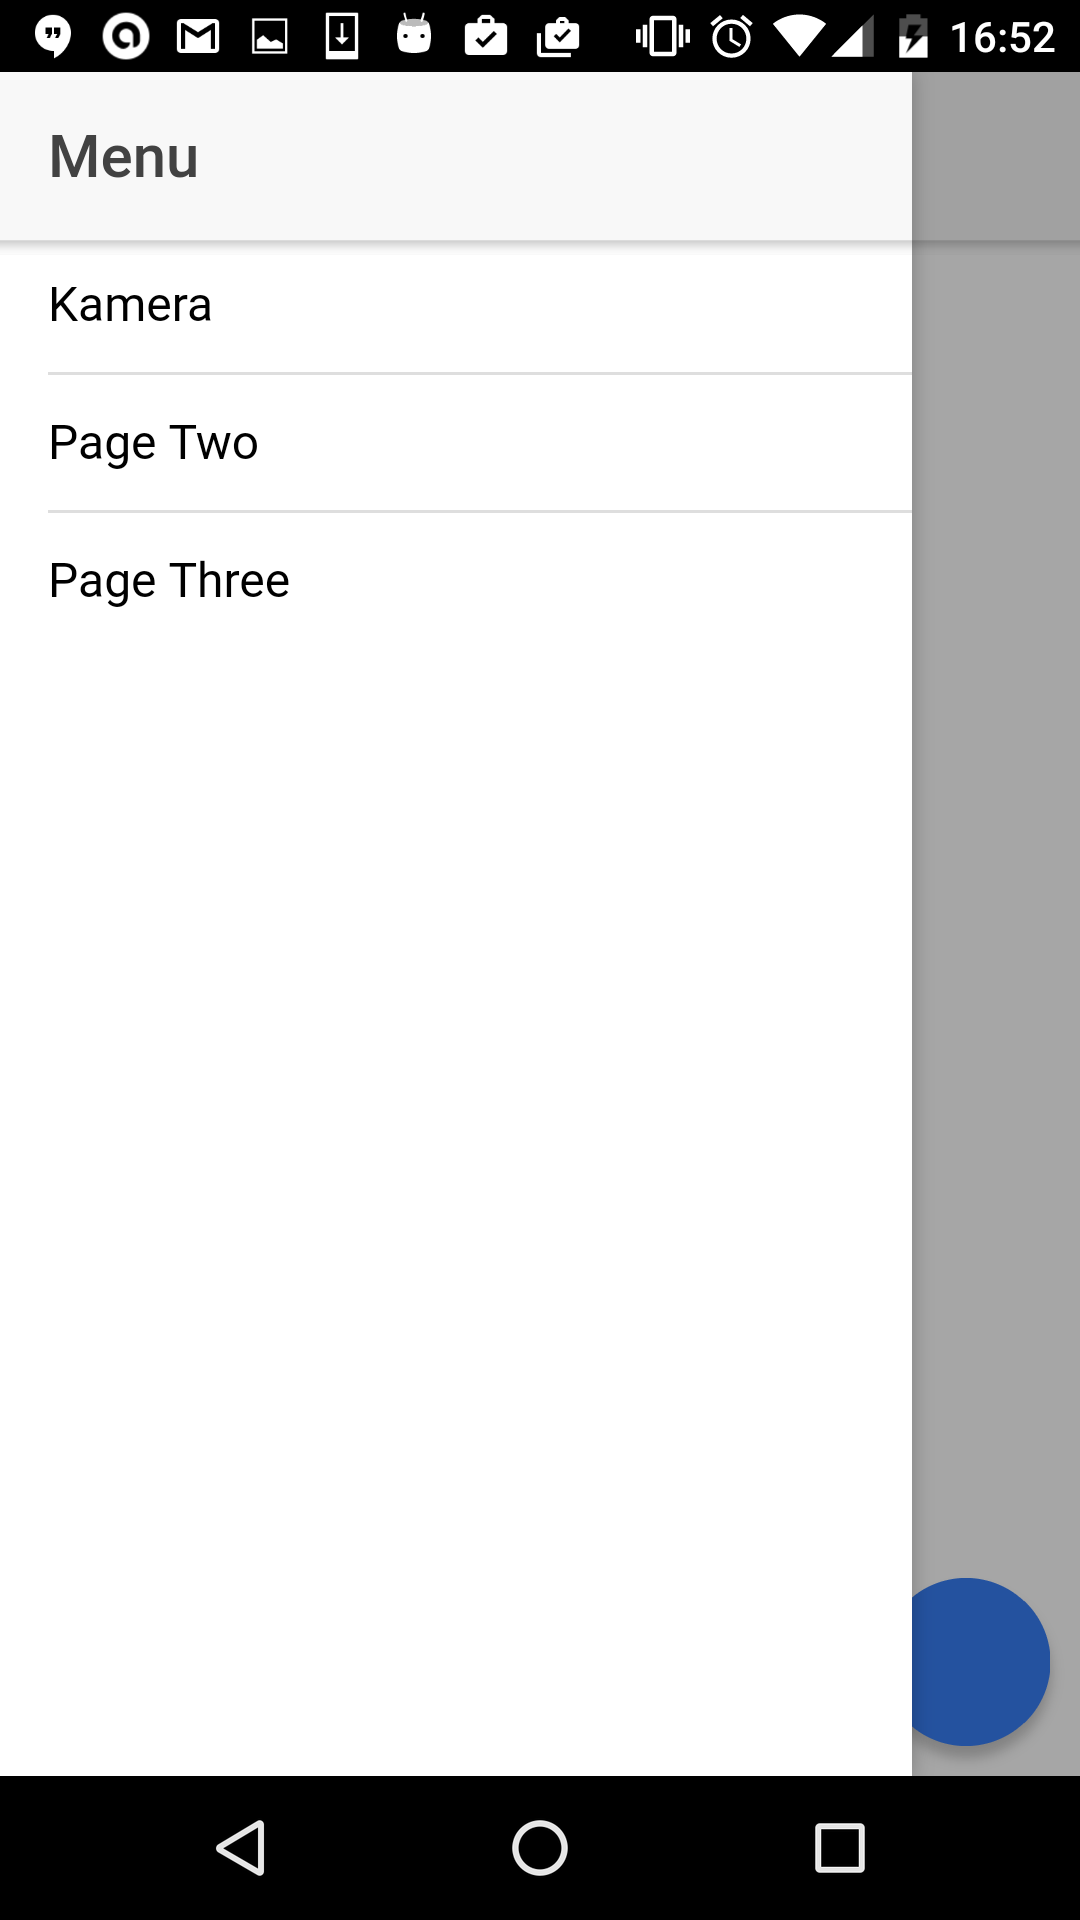
\includegraphics[width=0.4\textwidth]{Bilder/Screenshot_20170328-165235.PNG}
	\caption{Menü in der Ionic 2 Anwendung}
	\label{fig:MenuIonic}
\end{figure} 

In den HTML-Dateien der einzelnen Seiten, in denen deren Layout definiert wird, muss nur noch seitenspezifisches Design implementiert werden, das Menü wird hier nicht weiter bearbeitet. Das Ionic Framework bietet hier auch direkt die Möglichkeit einen \textit{FloatingActionButton} zu benutzen, was dem nativen GUI-Design entgegenkommt (siehe Listing \ref{lst:FloatingActionButtonIonic}).

\begin{lstlisting}[caption=Deklaration eines \textit{FloatingActionButton}, label=lst:FloatingActionButtonIonic, language=html]
<ion-fab right bottom>
    <button ion-fab color="red" (click)="presentActionSheet()"></button>
  </ion-fab>
\end{lstlisting}

Im Gegensatz zur nativen Android Entwicklung müssen UI-Elemente, die in der Layout-Datei, hier in einer HTML-Datei, deklariert wurden, nicht mehr im Konstruktor der zugehörigen Source-Datei initialisiert werden. Bei Buttons, die durch Klicken eine Aktion ausführen sollen, wird die auszuführende Methode in der HTML-Datei dem Button zugewiesen, wie oben in Listing \ref{lst:FloatingActionButtonIonic} zu erkennen ist. 

\subsection*{Sensoren}

Ionic 2 bringt ein \textit{native} Paket mit sich, in dem Klassen definiert sind, welche Cordova-Plugins kapseln und so in TypeScript genutzt werden können. Es existieren bisher nicht für alle Sensoren kapselnde Klassen, sondern nur für den Beschleunigungssensor, das Magnetometer und GPS. Möchte man andere Sensoren nutzen, so ist man darauf angewiesen, ein den Anforderungen entsprechenden Cordova-Plugin zu finden oder ein eben solches selber zu schreiben. Bei der Einbindung und Nutzung eines solchen Cordova-Plugins ist man allerdings wieder dazu gezwungen JavaScript zu nutzen. Dies wird in dieser Arbeit nicht umgesetzt, sondern es wird sich auf das beschränkt, was das Ionic 2 Framework direkt mitliefert.
\\
\\
Um beispielsweise mit Ionic 2 auf das Magnetometer zugreifen zu können, muss zunächst ein bestimmtes Cordova-Plugin installiert werden. Auf der Homepage des Ionic Frameworks sind diese Informationen in der Dokumentation des \textit{native} Pakets zu finden. Im Fall des Magnetometers muss das Plugin \textit{Device Orientation} heruntergeladen und installiert werden. Dies erfolgt über 2 Kommandos (Siehe Listing \ref{lst:InstallationCordovaPlugin}), welche in einer Kommando-Shell ausgeführt werden müssen, in welcher zunächst in den Root-Ordner der Anwendung navigiert wurde. 

\begin{lstlisting}[caption=Installation des Cordova-Plugins für das Magnetometer, label=lst:InstallationCordovaPlugin, language=bash]
ionic plugin add cordova-plugin-device-orientation
npm install --save @ionic-native/device-orientation
\end{lstlisting}

Anders als bei der nativen Android Entwicklung oder auch bei der Entwicklung mit dem Framework Xamarin, müssen bei der Verwendung von Hardware-Komponenten mit dem Ionic Framework keine Berechtigungen manuell der Anwendung hinzugefügt werden. Die nötigen Berechtigungen bringt das Cordova-Plugin mit sich. Um das installierte Cordova-Plugin in der Anwendung zu nutzen, müssen die dieses Plugin kapselnden Klassen aus dem \textit{native} Paket importiert werden (siehe Listing \ref{lst:ImportDeviveOrientation}). 

\begin{lstlisting}[caption=Import der Klassen für die Nutzung des Magnetometers aus dem  \textit{native} Paket von Ionic 2, label=lst:ImportDeviveOrientation, language=Java]
import {DeviceOrientation, DeviceOrientationCompassHeading} from 'ionic-native';
\end{lstlisting}

Anschließend können die importierten Klassen und ihre Methoden dazu genutzt werden, Daten des Sensors auszulesen und anzuzeigen. Um einmalig den aktuellen Wert des Magnetometers auszulesen, kann die Methode \textit{getCurrentHeading()} der Klasse \textit{DeviceOrientation} verwendet werden. Der Rückgabewert dieser Methode ist vom Typ \textit{DeviceOrientationCompassHeading}. Mithilfe der Methode \textit{magneticHeading()} kann nun der aktuelle Sensorwert aus dem \textit{DeviceOrientationCompassHeading}-Objekt gelesen und weiter genutzt werden. Möchte man den Sensor in einem regelmäßigen Intervall auslesen, so wird die Methode \textit{watchHeading()} benötigt. Da es bei einer Kompass-Anwendung sinnvoll ist, immer den aktuellen Sensorwert anzeigen zu lassen ohne manuell aktualisieren zu müssen, werden die Sensordaten hier mittels der Methode \textit{watchHeading()} ausgelesen und angezeigt (siehe Listing \ref{lst:getDataDeviceOrientation}). 

\begin{lstlisting}[caption=Auslesen der Daten des Magnetometers mithilfe der Methode \textit{watchHeading()}, label=lst:getDataDeviceOrientation, language=Java]
platform.ready().then(() => {
          DeviceOrientation.watchHeading().subscribe(
            (data: DeviceOrientationCompassHeading) => this.orientation2 = data.magneticHeading.toString()
          );
      });
\end{lstlisting}

\subsection*{Kameras}

Für die Nutzung der Kamera gibt es ähnlich wie oben bei der Sensornutzung beschrieben eine kapselnde Klasse im \textit{native} Paket des Ionic 2 Frameworks. Der Name dieser Klasse ist simpel \textit{Camera}. Um diese Klasse zu nutzen muss ebenfalls wie bei der Sensornutzung vorab ein Cordova-Plugin installiert werden. In diesem Fall ist es das Plugin \textit{Camera}. Die Installation erfolgt über die Kommando-Shell. 
\\
\\
Ruft man die Methode \textit{getPicture()} der Klasse \textit{Camera} auf, so wird über das installierte Cordova-Plugin die native Android Kamera-Anwendung gestartet. Der Methode \textit{getPicture()} können hierbei noch weitere Optionen, zum Beispiel bezüglich der Bildqualität, mitgegeben werden (siehe Listing \ref{lst:CameraIonic}). 

\begin{lstlisting}[caption=Aufruf der Android Kamera-Anwendung über die Methode \textit{getPicture()}, label=lst:CameraIonic, language=Java]
public takePicture(sourceType) {
  
  var options = {
    quality: 100,
    sourceType: sourceType,
    saveToPhotoAlbum: true,
    correctOrientation: true
  };
	Camera.getPicture(options).then((imagePath) => {
      
        var currentName = imagePath.substr(imagePath.lastIndexOf('/') + 1);
        var correctPath = imagePath.substr(0, imagePath.lastIndexOf('/') + 1);
        this.copyFileToLocalDir(correctPath, currentName, this.createFileName());
      
    }
}
\end{lstlisting}

Wie man oben in Listing \ref{lst:CameraIonic} sehen kann, wird, nachdem mit der Android Kamera-Anwendung ein Foto geschossen wurde, ein Dateiname mit der Methode \textit{createFileName()} für dieses generiert und die Methode \textit{copyFileToLocalDir} aufgerufen, in der das Speichern dieses Bildes implementiert ist. Die Methode \textit{getPicture()} liefert hier unter anderem den Pfad, unter dem die Android Kamera-Anwendung das Bild zwischenspeichert, zurück.

\subsection*{Speicherzugriffe}

Die Speicherzugriffe zum Speichern und laden geschossener Fotos werden ebenfalls über ein Cordova-Plugin (\textit{File} und \textit{File Transfer}) abgehandelt. Die benötigten Klassen aus dem \textit{native} Paket, welche importiert werden müssen sind \textit{File} und \textit{FilePath}. Wie oben in Listing \ref{lst:CameraIonic} schon zu sehen war, wird das Speichern in der Methode \textit{copyFileToLocalDir()} vorgenommen. Der Methode werden dafür der aktuelle Pfad, der Name des Bildes und ein neuer Name übergeben. Mit der Methode \textit{copyFile()} wird das Bild nun in dem angegebenen Ordner abgelegt. In diesem Fall ist das \textit{cordova.file.externalDataDirectory}. Das \textit{externalDataDirectory} des Cordova-Plugins entspricht dem \textit{External Storage} von Android. Der eben beschriebene Speichervorgang ist unten in Listing \ref{lst:SavePictureIonic} zu sehen. 
\clearpage

\begin{lstlisting}[caption=Methode \textit{copyFileToLocalDir()} zum Speichern der aufgenommenen Bilder, label=lst:SavePictureIonic, language=Java]
private copyFileToLocalDir(namePath, currentName, newFileName) {
    File.copyFile(namePath, currentName, cordova.file.externalDataDirectory, newFileName).then(success => {
      this.lastImage = newFileName;
    }, error => {
      this.presentToast('Error while storing file.');
    });
  }
\end{lstlisting}


\section{Implementierung mit React Native}

Wie schon zuvor bei der Entwicklung mit dem Ionic 2 Framework und Cordova muss auch für die Entwicklung mit dem React Native Framework Node.js installiert sein. Anschließend wird das React Native Kommandozeilen Interface installiert. Eine React Native Anwendung basiert auf React. React, oder auch ReactJS ist ein JavaScript Framework zum Designen von Benutzeroberflächen\footcite{React}. Der Quellcode ist teilweise in JavaScript, teils in HTML geschrieben. Zum Entwickeln mit React Native kann ein beliebiger Editor verwendet werden. Zum optimalen Vergleich wird auch die React Native Anwendung gegen die API 23, die Major Version 6 (Marshmallow), kompiliert.  

\subsection*{Grafische Benutzeroberfläche}

Im Gegensatz zur Entwicklung mit dem Ionic Framework und auch mit Xamarin, steht die Implementierung der grafischen Benutzeroberfläche und die der Fachlogik nicht in getrennten Dateien. Die grafischen Elemente werden zwar wie bei dem Ionic Framework in HTML implementiert, dieser HTML-Code ist allerdings im JavaScript-Quellcode eingebettet. 
\\
\\
React Native unterstützt bereits einige gängige UI-Elemente, wie zum Beispiel den \textit{FloatingActionButton}. Sollte man allerdings etwas Spezielles benötigen, was nicht in den React Native Bibliotheken enthalten ist, so können auch manuell weitere native Komponenten der Anwendung hinzugefügt werden. Die Basis-Quellcode-Dateien für die beiden Systeme Android und iOS liegen direkt unter dem Root-Verzeichnis der Anwendung. Möchte man ausschließlich gemeinsamen Code verwenden, so kann man eine neue gemeinsame Basis-Quelldatei anlegen und in den plattformspezifischen Dateien diese importieren. 
\\
\\
Für ein wie in Kapitel \ref{OOAOODGUI} gefordertes Menü bietet das React Native Framework den sogenannten \textit{DrawerNavigator}. Um diesen zu nutzen muss er zunächst oben in der Basis-Quelldatei importiert werden (siehe Listing \ref{lst:ImportDrawerNavigator}).

\begin{lstlisting}[caption=Import der Klasse \textit{DrawerNavigator} für das Menü in React Native, label=lst:ImportDrawerNavigator, language=Java]
import { DrawerNavigator } from 'react-navigation';
\end{lstlisting}

Eine Seite, hier ein Screen, wird durch eine eigene Klasse dargestellt, welche von der Klasse \textit{React.Component} erben muss. Der Titel der Seite wird nebst anderen Einstellungen wie ein Icon in den statischen \textit{navigationOptions} festgelegt (siehe Listing \ref{lst:SeitentitelReactNative}).

\begin{lstlisting}[caption=Festlegen des Seitentitels, label=lst:SeitentitelReactNative, language=Java]
class MyHomeScreen extends React.Component {
  static navigationOptions = {
    drawer: () => ({
      label: 'Home',
      icon: ({ tintColor }) => (
        <Image source={require('./images/ic_home_black_24dp.png')} style={[styles.icon, {tintColor: tintColor}]}/>
      ),
    }),
  }
  ...
}
\end{lstlisting}

Zuletzt müssen die einzelnen Seiten, zu denen man navigieren können soll einem \textit{DrawerNavigator}-Objekt zugeordnet werden. Dies geschieht, wie man in Listing \ref{lst:DrawerNavigatorConfig} sehen kann in der Konstanten \textit{DrawerApp}. 
\clearpage

\begin{lstlisting}[caption=Konfiguration des \textit{DrawerNavigators}, label=lst:DrawerNavigatorConfig, language=Java]
const DrawerApp = DrawerNavigator({
  Home: {
    screen: MyHomeScreen,
  },
  Kamera: {
    screen: CameraRollGallery,
  },
  Senoren: {
    screen: CameraRollGallery,
  },
  ...
});
\end{lstlisting}

Nachfolgend ist in Abbildung \ref{fig:MenuReactNative} das Menü der React Native Anwendung dargestellt. Es lässt sich wie gewohnt über Wischen öffnen und schließen. Anders als die Menüs der anderen Frameworks und das native Menü hat das Menü der React Native Anwendung keinen integrierten Header.

\begin{figure}[h]
	\centering
	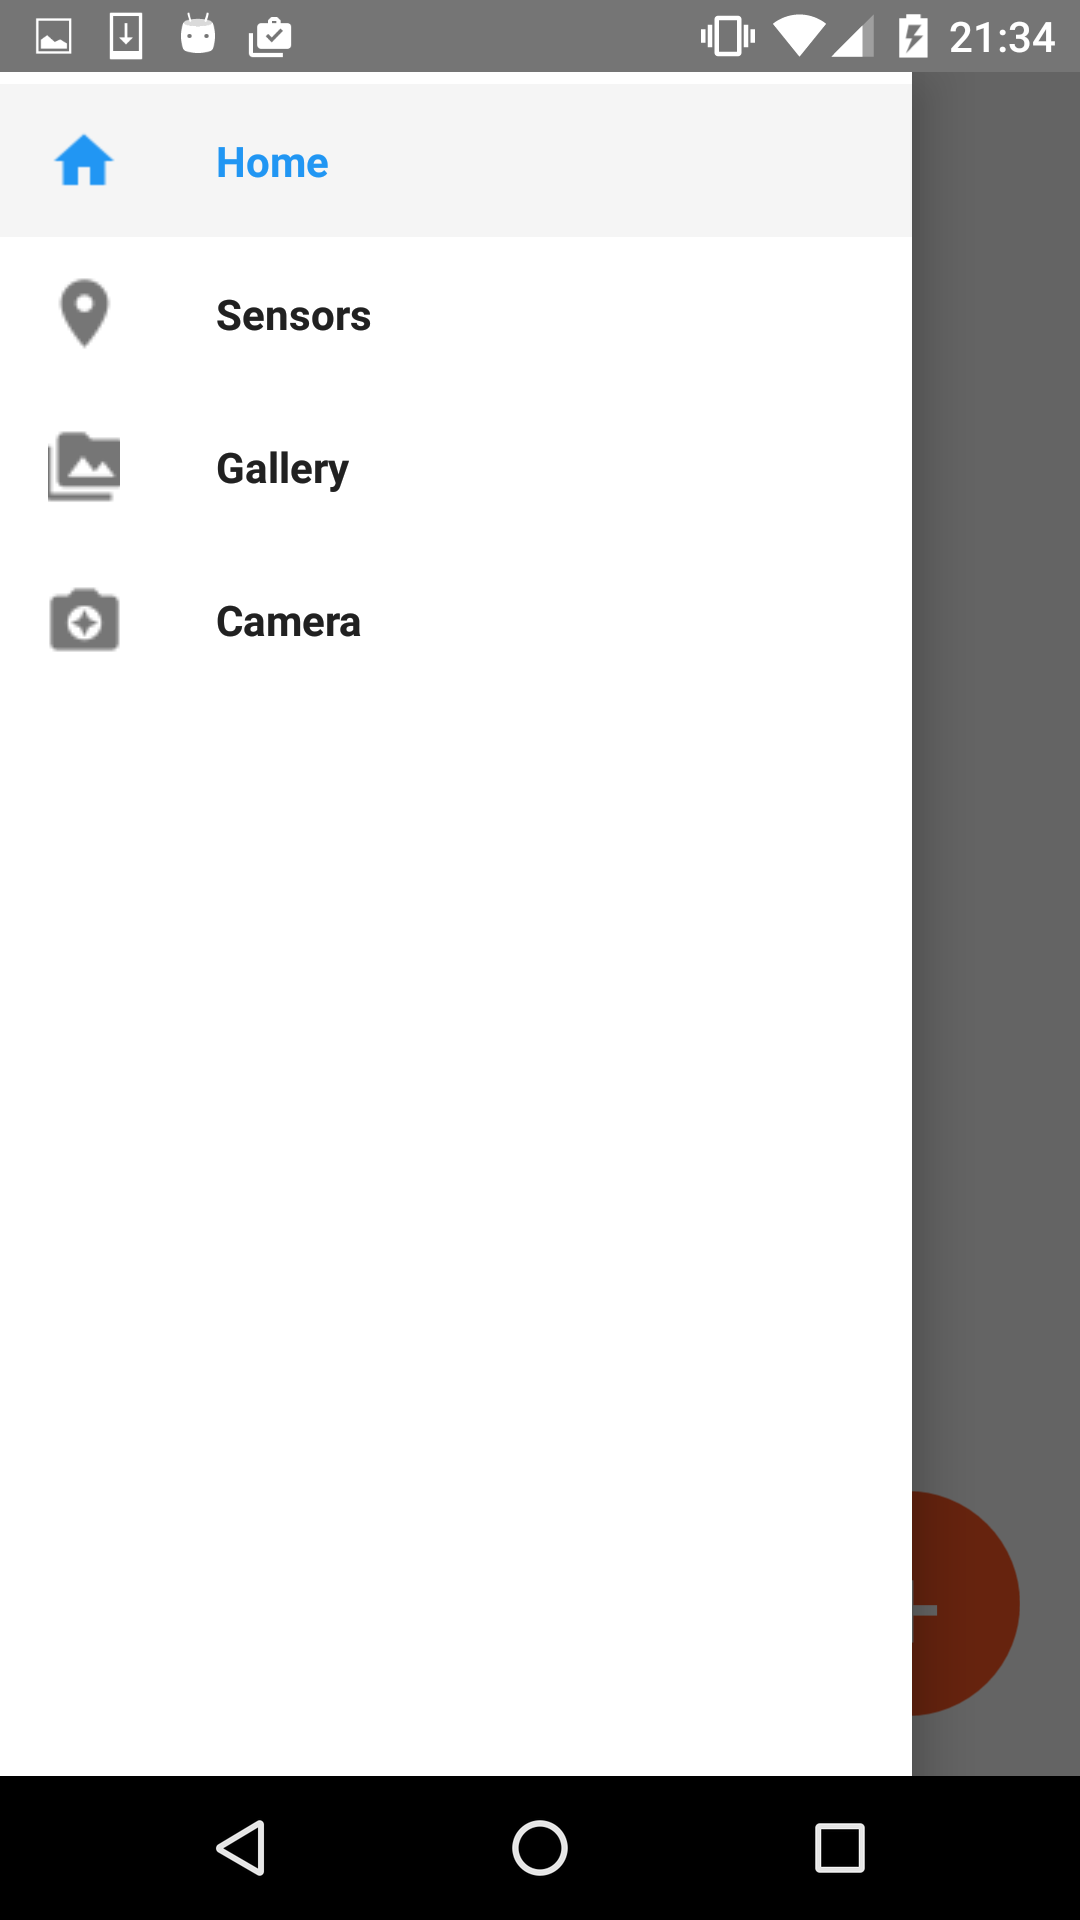
\includegraphics[width=0.4\textwidth]{Bilder/Screenshot_20170412-213445.PNG}
	\caption{Menü in der React Native Anwendung}
	\label{fig:MenuReactNative}
\end{figure}
\clearpage

Einen \textit{FloatingActionButton} bringt das React Native Framework nicht direkt mit. Ein \textit{TouchableHighlight}-Objekt lässt sich allerdings so modifizieren, dass es aussieht und sich verhält wie ein \textit{FloatingActionButton} von Android. Das \textit{TouchableHighlight}-Objekt wird in der \textit{render()}-Funktion der Klasse der Seite deklariert, auf dem der FAB zu sehen sein soll (siehe Listing \ref{lst:FABReactNative}). 

\begin{lstlisting}[caption=Deklaration eines \textit{TouchableHighlight}-Objekts als \textit{FloatingActionButton}, label=lst:FABReactNative, language=Java]
render() {
    return (
      <TouchableHighlight style={styles.addButton} underlayColor='#ff7043' onPress={() => this.props.navigation.navigate('Camera')}>
        <Text style={{fontSize: 40, color: 'white'}}>+</Text>
      </TouchableHighlight>
    );
  }
\end{lstlisting}

Über \textit{style=styles.addButton} wird dem Objekt sein Design zugeordnet. Das \textit{FloatingActionButton}-Design steckt dabei in dem Attribut \textit{addButton}. In diesem wurden Größe, Form, Position, Verhalten etc. definiert, wie in Listing \ref{lst:FABDesignReactNative} zu sehen ist.

\begin{lstlisting}[caption=Das \textit{FloatingActionButton}-Design, label=lst:FABDesignReactNative, language=Java]
addButton: {
    backgroundColor: '#ff5722',
    borderColor: '#ff5722',
    borderWidth: 1,
    height: 75,
    width: 75,
    borderRadius: 50,
    alignItems: 'center',
    justifyContent: 'center',
    position: 'absolute',
    bottom: 20,
    right:20,
    shadowColor: "#000000",
    shadowOpacity: 0.8,
    shadowRadius: 2,
    shadowOffset: {
      height: 1,
      width: 0
    }
},
\end{lstlisting} 

\subsection*{Sensoren}

Möchte man in einer React Native Anwendungen auf die Sensoren des Smartphones zugreifen, so bietet sich hierfür die \textit{react-native-sensor-manager}-Bibliothek an. Sensoren, auf die über den Sensor Manager zugegriffen werden können sind: der Beschleunigungssensor, das Gyroskop, das Magnetometer, der Lagesensor, das Thermometer, der Lichtsensor und der Näherungssensor. Das GPS ist direkt über die API des React Native Frameworks ansprechbar. 
\\
\\
Um den Sensor Manager zu nutzen muss dieser zunächst über die Kommando-Shell installiert via \textit{npm} installiert und die Bibliothek verlinkt werden (siehe Listing \ref{lst:InstallationSensorManagerRN}).

\begin{lstlisting}[caption=Installation und Verlinkung der Bibliothek \textit{react-native-sensor-manager}, label=lst:InstallationSensorManagerRN, language=bash]
npm i react-native-sensor-manager --save
react-native link react-native-sensor-manager
\end{lstlisting}

Fehlen Berechtigungen, so können diese manuell im \textit{AndroidManifest} unter \textit{/android/app/src/main} hinzugefügt werden. Anschließend muss die Klasse \textit{SensorManager} aus dem Paket \textit{NativeModules} in der Quelldatei importiert werden (siehe Listing \ref{lst:ImportSensorManager}). 

\begin{lstlisting}[caption=Import der \textit{SensorManager}-Klasse, label=lst:ImportSensorManager, language=Java]
import { SensorManager } from 'NativeModules';
\end{lstlisting}

Das Auslesen und Präsentieren von Sensordaten wird in diesem Fall wieder anhand des Näherungssensors gezeigt. Der Sensor wird im Konstruktor der Seite gestartet, auf der die Daten des Sensors präsentiert werden sollen. Über die Methode \textit{startProximitx()} wird der Näherungssensor gestartet (siehe Listing \ref{lst:ProximityData}). Die der Methode übergebene Zahl '100' bedeutet eine Verzögerung von mindestens 100ms zwischen den Events. Mithilfe der Klasse \textit{DeviceEventEmitter} aus der \textit{react-native}-Bibliothek wird ein \textit{Listener} hinzugefügt. 
\clearpage

\begin{lstlisting}[caption=Auslesen und Anzeigen der Daten des Näherungssensors, label=lst:ProximityData, language=Java]
constructor(props) {
    super(props);
    SensorManager.startProximity(100);
    DeviceEventEmitter.addListener('Proximity', function (data) {
        if (data.isNear === true) {
          ToastAndroid.show('Near',ToastAndroid.SHORT);
        } else {
          ToastAndroid.show('Far',ToastAndroid.SHORT);
        }
    });
}
\end{lstlisting}

\subsection*{Kameras}

Um die Kamerafunktionen des Smartphones in einer React Native Anwendung nutzen zu können, muss zunächst die Bibliothek \textit{react-native-camera} via \textit{npm} installiert werden. Anschließend muss die Bibliothek noch mit dem Befehl \textit{react-native link react-native-camera} verknüpft und in der Quelldatei importiert werden. Gegebenenfalls müssen noch Berechtigungen im \textit{AndroidManifest}, welches unter \textit{/android/app/src/main} liegt, hinzugefügt werden. 
\\
\\
Anders als beim Ionic und Xamarin Framework gibt es im React Native Framework direkte Möglichkeit die Android Kameraanwendung innerhalb der React Native Anwendung zu starten. Aus diesem Grund wurden Elemente wie der Auslösebutton und die Blitzeinstellungen manuell der Seite mit der Kamerafunktion hinzugefügt. Die Designs der einzelnen UI-Elemente wurden wie das Design des \textit{FloatingActionButtons} unter \textit{const styles} hinzugefügt. Listing \ref{lst:styleCaptureButton} zeigt beispielhaft das Design des Auslösebuttons.

\begin{lstlisting}[caption=Das Design des Auslösebuttons für die Kamerafunktion, label=lst:styleCaptureButton, language=Java]
const styles = StyleSheet.create({
...
captureButton: {
    padding: 15,
    backgroundColor: 'white',
    borderRadius: 40,
  },
...
});
\end{lstlisting} 

In der \textit{render()}-Funktion werden die einzelnen Elemente der Benutzeroberfläche deklariert. Das oben (Listing \ref{lst:styleCaptureButton}) gezeigte Design wird hier einem \textit{TouchableOpacity}-Objekt zugeordnet, welches dann den Auslösebutton darstellt (siehe Listing \ref{lst:CaptureButton}). 

\begin{lstlisting}[caption=Deklaration eines \textit{TouchableOpacity}-UI-Objekts für die Darstellung des Auslösebuttons der Kamera, label=lst:CaptureButton, language=Java]
render() {
    return (
		...
			<TouchableOpacity
                style={styles.captureButton}
                onPress={this.takePicture}
            >
              <Image source={require('./images/ic_photo_camera_36pt.png')}/>
            </TouchableOpacity>
		...
	);
}
\end{lstlisting} 

Wird der Button gedrückt, so wird die Methode \textit{takePicture()} aufgerufen, welche nachfolgend in Listing \ref{lst:takePictureReactNative} dargestellt ist. Innerhalb dieser Methode wird die Methode \textit{capture()} des Kameraobjekts \textit{camera} aufgerufen. Dies ist die eigentliche Auslöse-funktion der Kamera. Das geschossene Bild wird automatische mit Timestamp im Namen im öffentlichen Bilder-Verzeichnis des Android Smartphones gespeichert. 

\begin{lstlisting}[caption=Die Methode \textit{takePicture()} zum Auslösen der Kamera, label=lst:takePictureReactNative, language=Java]
takePicture = () => {
    if (this.camera) {
      this.camera.capture()
        .then((data) => console.log(data))
        .catch(err => console.error(err));
    }
}
\end{lstlisting} 

Das oben in Listing \ref{lst:takePictureReactNative} verwendete Kameraobjekt \textit{camera} wird im Konstruktor der Klasse initialisiert (siehe Listing \ref{lst:InitialisierungCameraRN} unten). Hier werden dem Objekt Voreinstellungen mitgegeben. Beim Start der Kameraanwendung ist in diesem Fall die Rückkamera des Smartphones aktiv und der Blitz ist auf automatisch eingestellt. 
\clearpage

\begin{lstlisting}[caption=Initialisierung des Kameraobjekts im Konstruktor, label=lst:InitialisierungCameraRN, language=Java]
...
camera: {
        aspect: Camera.constants.Aspect.fill,
        captureTarget: Camera.constants.CaptureTarget.cameraRoll,
        type: Camera.constants.Type.back,
        orientation: Camera.constants.Orientation.auto,
        flashMode: Camera.constants.FlashMode.auto,
},
isRecording: false
...
\end{lstlisting}

Für das Ändern des Blitzmodus wird ein UI-Element, welches selbst den aktuell ausgewählten Blitzmodus anzeigt, oben rechts im Bild gesetzt. Durch tippen auf dieses Element wird durch die 3 verschiedenen Blitzoptionen \textit{on}, \textit{off} und \textit{auto} rotiert. Listing \ref{lst:FlashSwitchElement} zeigt die Initialisierung dieses Elements.  

\begin{lstlisting}[caption=Initialisierung des UI-Elements zum Wechseln des Blitzmodus, label=lst:FlashSwitchElement, language=Java]
...
<TouchableOpacity
	style={styles.flashButton}
    onPress={this.switchFlash}
>
    <Image source={this.flashIcon}/>
</TouchableOpacity>
...
\end{lstlisting}

Die Methode \textit{switchFlash()} übernimmt das Rotieren durch die Blitzoptionen. Wie man in Listing \ref{lst:switchFlash} erkennen kann, besitzt das Kameraobjekt ein Attribut \textit{flashMode}, welches entsprechend dem momentan ausgewählten Modus bei Aufruf der Methode \textit{switchFlash()} einen anderen Modus zugewiesen bekommt. Die Methode \textit{flashIcon()} ist wie die Methode \textit{switchFlash()} aufgebaut, nur das in ihr das entsprechende Icon des UI-Elements für die Blitzoptionen gesetzt wird.
\clearpage

\begin{lstlisting}[caption=Die Methode \textit{switchFlash()} für das Ändern des Blitzmodus, label=lst:switchFlash, language=Java]
switchFlash = () => {
    let newFlashMode;
    const { auto, on, off } = Camera.constants.FlashMode;

    if (this.state.camera.flashMode === auto) {
      newFlashMode = on;
    } else if (this.state.camera.flashMode === on) {
      newFlashMode = off;
    } else if (this.state.camera.flashMode === off) {
      newFlashMode = auto;
    }

    this.setState({
      camera: {
        ...this.state.camera,
        flashMode: newFlashMode,
      },
    });
}
\end{lstlisting}

Die manuell erstellte Benutzeroberfläche für die Bedienung der Kamerafunktionen in der React Native Anwendung ist nachfolgend in Abbildung \ref{fig:KameraReact} dargestellt. In der linken oberen Ecke ist das Element zum Wechseln zwischen Rück- und Frontkamera. Die Funktionsweise dieses Elements entspricht der der Blitzoptionen. 
\clearpage

\begin{figure}[h]
	\centering
	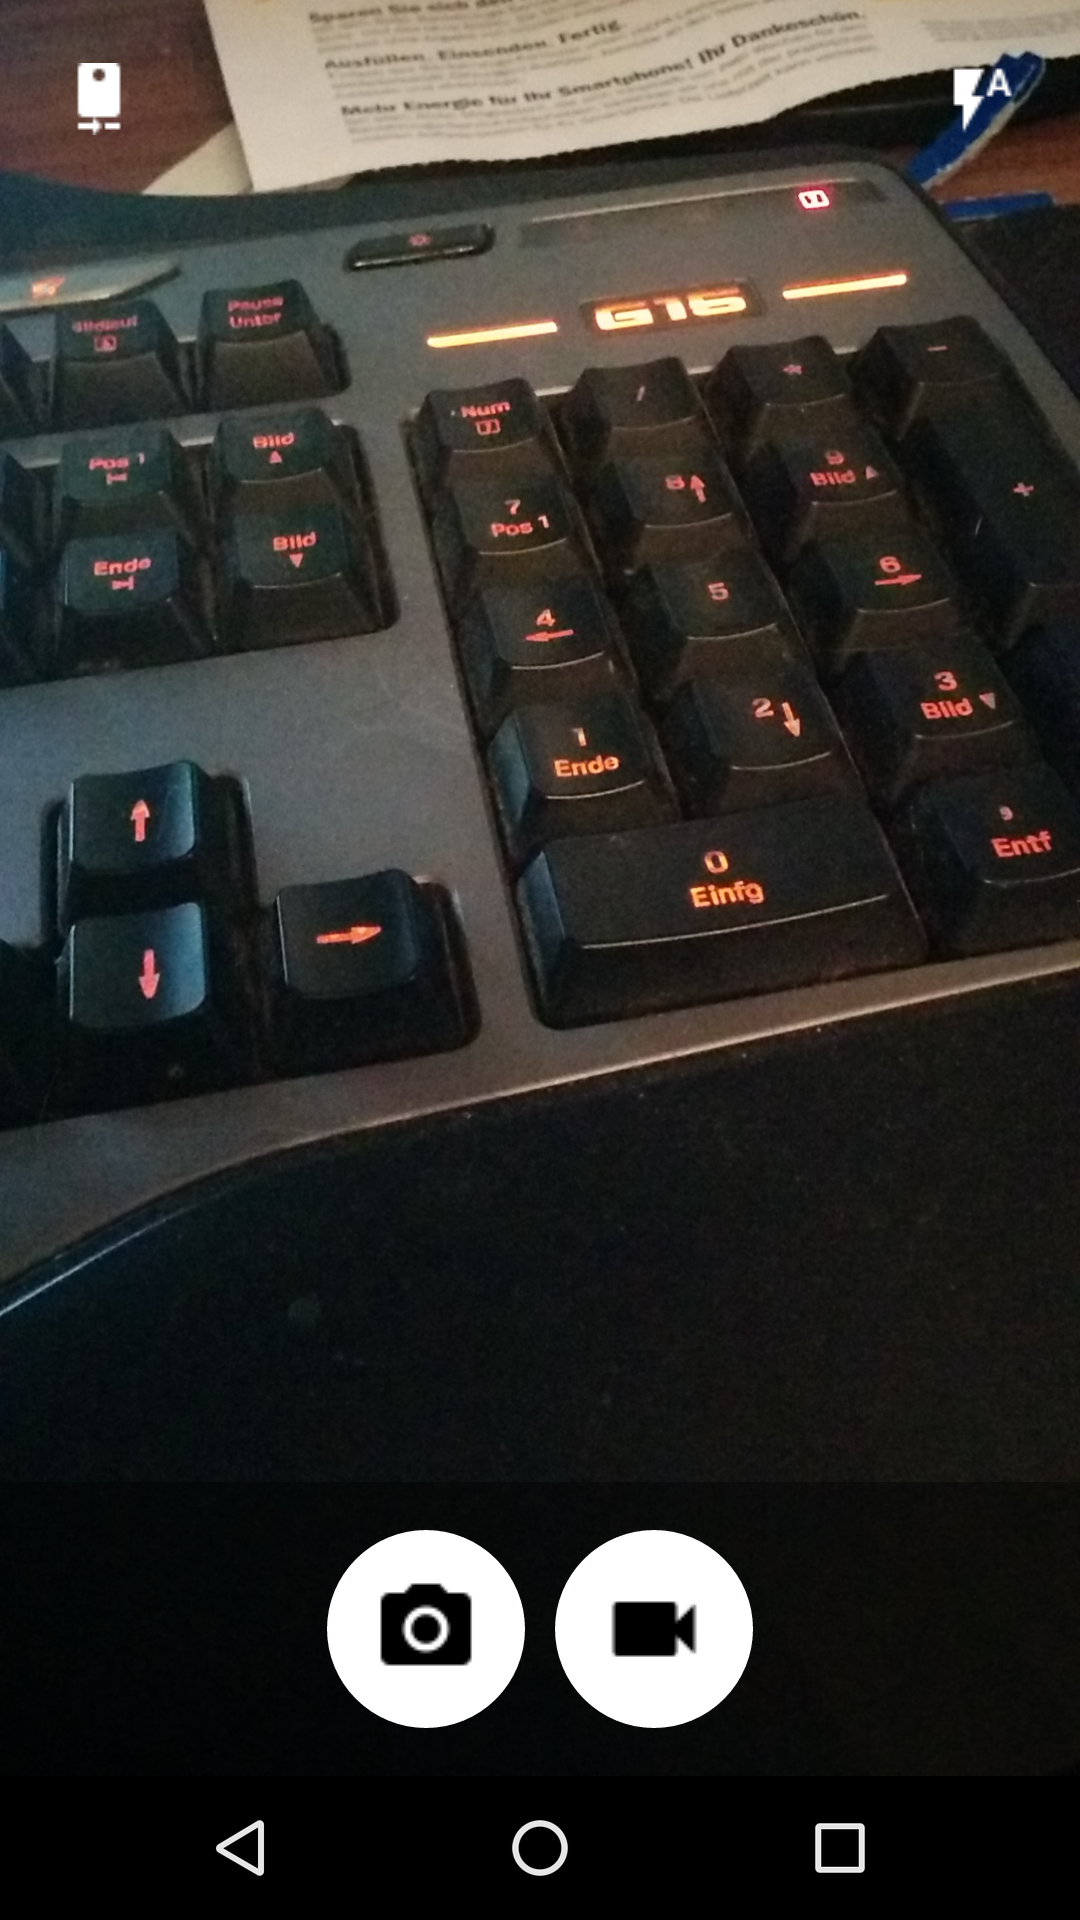
\includegraphics[width=0.4\textwidth]{Bilder/Screenshot_20170412-213200.PNG}
	\caption{Kamerafunktion in der React Native Anwendung}
	\label{fig:KameraReact}
\end{figure}

\subsection*{Speicherzugriffe}

Um die geschossenen Fotos, oder bei Bedarf auch weitere Bilder, die Auf dem Smartphone gespeichert sind, zu laden wird die Methode \textit{getPhotos()} der Klasse \textit{CameraRoll} aufgerufen (siehe Listing \ref{lst:getPhotosReactNative}). Die Klasse \textit{CameraRoll} ist aus dem Plugin \textit{rn-camera-roll}, welches zuvor über \textit{npm} installiert und anschließend in der Quelldatei importiert werden musste. Der Methode \textit{getPhotos()} können hierbei verschiedene Optionen mitgegeben werden, die unter anderem angeben, welche Bilddateien geladen werden sollen. Ein paar Möglichkeiten sind hier \textit{Library}, \textit{All} oder \textit{Album}. Per Default wird \textit{SavedPhotos} mitgegeben. 
\clearpage

\begin{lstlisting}[caption=Aufruf der Methode \textit{getPhotos()} für die Anzeige gespeicherter Bilder in einer Galerie, label=lst:getPhotosReactNative, language=Java]
fetchPhotos(count = PHOTOS_COUNT_BY_FETCH, after) {
    CameraRoll.getPhotos({
      first: count,
      after,
    }, this.onPhotosFetchedSuccess.bind(this), this.onPhotosFetchError.bind(this));
  }
\end{lstlisting} 
\chapter{Auswertung}

Im folgenden Kapitel wird die Auswertung anhand der in Kapitel (X) aufgestellten Bewertungskriterien beschrieben. Zu den einzelnen Kategorien (siehe Kapitel (X)) wird der jeweilige ausgefüllte Abschnitt der Bewertungsmatrix dargestellt und erläutert. 

\section{Kosten und Lizenz}

Nachfolgende Abbildung (X) zeigt den Abschnitt 'Kosten und Lizenz' der ausgefüllten Bewertungsmatrix.

\begin{figure}[h]
	\centering
	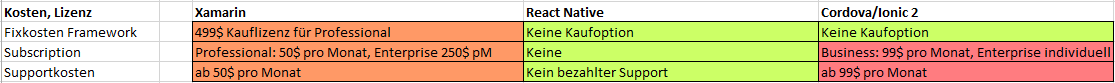
\includegraphics[width=1\textwidth]{Bilder/Auswertung_KostenLizenz.PNG}
	\caption{Bewertungsmatrix Kategorie Kosten und Lizenz}
	\label{fig:AuswKostLiz}
\end{figure}

Das Xamarin Framework gibt es in einer kostenlosen Community-Version und in den kostenpflichtigen Versionen 'Professional' und 'Enterprise'. Die kostenlose Community-Version gibt es für Windows inklusive einer Community-Version von Visual Studio und für Apple mit der IDE 'Xamarin Studio'. Die Preise der kostenpflichtigen Versionen richten sich nach den Preisen der entsprechenden Version der IDE Visual Studio. Die Professional-Version kann für 499\$ ohne Subscription oder für 1199\$ mit Subscription erworben werden. Eine Subscription hält 2 Jahre, ein Auffrischen danach kostet 799\$. Die Enterprise-Version kann nur mit Subscription erworben werden. Sie kostet 5999\$ und ein Auffrischen nach Ablauf der 2 Jahre kostet 2569\$. Einen technischer Support  erhält man mit jeder Subscription, das bedeutet ab umgerechnet 50\$ pro Monat. E-Mail-Support erhalten alle Business- und Enterprise-Kunden. Zusätzlich zu allen Modellen kann die Xamarin Test-Cloud ab einen monatlichen Preis von 99\$ genutzt werden.
\\
\\
Für das Framework React Native gibt es keine kostenpflichtigen Versionen. 
\\
\\
Für das Framework Cordova gibt es ebenfalls keine kostenpflichtigen Modelle. Das Framework Ionic bietet dagegen folgende Varianten an: eine kostenlose Community-Version und die kostenpflichtigen Versionen 'Indie', 'Business' und 'Enterprise'. Im Gegensatz zu den kostenpflichtigen Modellen bei Xamarin, fallen bei den Modellen von Ionic monatliche Subscription-Gebühren an. Die Indie-Variante kostet 25\$ pro Monat und die Business-Variante kostet 99\$ pro Monat. Für die Enterprise-Version gibt es einen individuellen Preis auf Anfrage. Ab der Business-Variante erhält man E-Mail-Support, das bedeutet ab 99\$ pro Monat. Möchte man die Ionic Test Cloud nutzen, so kostet dies 20\$ pro Monat und Anwendung.  

\section{Support und Community}

Die Bewertung der einzelnen Frameworks in der Kategorie 'Support und Community' ist in nachfolgender Abbildung (X) dargestellt.

\begin{figure}[h]
	\centering
	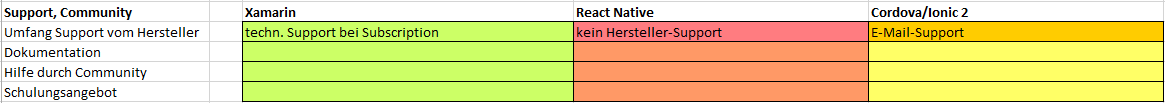
\includegraphics[width=1\textwidth]{Bilder/Auswertung_SupportCommunity.PNG}
	\caption{Bewertungsmatrix Kategorie Support und Community}
	\label{fig:AuswSuppComm}
\end{figure}

Beim Xamarin Framework wird ein technischer Support mit Erwerb einer Subscription angeboten. Zudem bekommen alle Kunden, die mindestens die 'Professional'-Version des Frameworks käuflich erworben haben einen E-Mail-Support. 
\\
Auf der Homepage von Xamarin ist im 'Developer Center' eine ausführliche Dokumentation inklusive API-Spezifikation zu finden. Zusätzlich hat man dort Zugriff auf Guides zu verschiedenen Funktionalitäten und Thematiken mit Beispielen und Code-Rezepten. Allein auf GitHub stehen über 150 öffentliche Repositories zur Verfügung. Zusätzlich hat man noch Zugriff auf ein FAQ, welches bei gängigen Problemen mit der Installation und Entwicklung mit Xamarin hilft. 
\\
Xamarin betreibt ein eigenes Forum mit mehreren Unterforen zu Themen wie Android, iOS, Tools etc. Es befinden sich über 80.000 Threads mit über 400.000 Posts in diesem Forum (Stand Februar 2017). Zusätzlich zum Xamarin Forum sind bei der 'Stack Overflow'-Community\footcite{StackOverfolw} noch über 55.000 Threads, die sich mit Themen zu Xamarin beschäftigen, zu finden. 
\\
Was Schulungen betrifft, so bieten die 'Xamarin Consulting Partners' sowohl Präsenz- als auch Videokonferenz-Schulungen an. Eine Präsenzschulung kann für 2-10 Tage gebucht werden und kostet dabei 1500\$ pro Tag plus Reisekosten. Schulungen via Konferenzschaltung können für 2-6 Stunden gebucht werden und kosten 200\$ pro Stunde. Neben diesen Schulungen bietet Xamarin auch Video Tutorials und Webinare an. 
\\
\\
Ionic bietet allen Kunden, die mindestens die 'Business'-Version käuflich erworben haben, einen E-Mail-Support an. 
\\
Ähnlich zum Xamarin 'Developer Center' bietet auch Ionic eine umfangreiche Dokumentation mit API Spezifikation an. Guides zu verschiedensten Themen wie 'Third Party Libraries' und einzelne Anwendungsfunktionalitäten, sowie Video-Crash-Kurse sind ebenfalls auf der Homepage von Ionic zu finden. Besonders ausführlich ist die große Übersicht sämtlicher verfügbarer UI-Elemente. Zu jedem UI-Element ist Beispielcode hinterlegt und auf einem eingeblendeten Emulator kann man sich jedes Element in den 3 Versionen iOS, Android und Windows Phone ansehen. Beispielcode und Links zu GitHub-Repositories zu einzelnen Funktionalitäten sind ebenfalls vorhanden. Zusätzlich bietet Ionic, wie Xamarin auch, ein FAQ an. 
\\
Ionic betreibt ein eigenes Forum, indem sich bereits über 30.000 Threads zu verschiedenen Themen befinden. Im 'Stack Overflow'-Forum\footcite{StackOverfolw} befinden sich weitere über 35.000 Threads über Ionic-bezogene Themen. Allerdings thematisieren nur knapp 7.000 Threads die Version Ionic 2. 
\\
Schulungen werden zwar keine von Ionic selbst angeboten, jedoch gibt es die sogenannten 'Trusted Partners'. Dies sind Unternehmen, die auf Anfrage bei der Umsetzung einer Ionic Anwendung unterstützen oder sogar die Implementierung komplett übernehmen. Auf der Homepage von Ionic gibt es zudem noch Buchempfehlungen und Links zu kostenpflichtigen eLearning-Kursen.
\\
\\
Im Gegensatz zu den Frameworks Xamarin und Ionic bietet React Native keinen Hersteller-Support wie E-Mail-Support oder ähnliches an.
\\
Was den Umfang der Dokumentation anbelangt, so bietet auch React Native Erläuterungen und Beispiel-Code zur Verwendung verschiedener Funktionalitäten, sowie eine API Spezifikation auf der Homepage an. Der Code vieler Plugins, die genutzt werden können, kann auf GitHub eingesehen werden. Auf der Homepage von React Native finden sichzudem noch Buchempfehlungen.
\\
React Native betreibt zwar kein eigenes Forum, es gibt dafür allerdings eine Facebook-Gruppe, in der über React Native-bezogene Themen diskutiert wird. In dieser Gruppe befinden sich über 12.500 Mitglieder (Stand Februar 2017). Im 'Stack Overflow'-Forum\footcite{StackOverfolw} gibt es über 18.000 Threads mit React Native-bezogenen Themen. 
\\
Von React Native selbst werden keine Schulungen, Video-Kurse oder dergleichen angeboten. 

\section{Entwicklung}

Die ausgefüllte Bewertungsmatrix für die Kategorie 'Entwicklung' ist in nachfolgender Abbildung (X) dargestellt.

\begin{figure}[h]
	\centering
	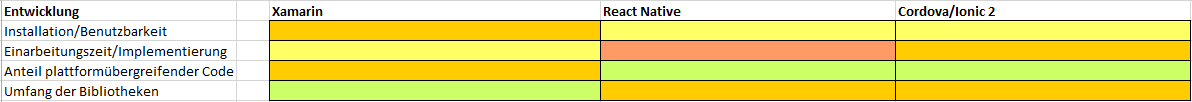
\includegraphics[width=1\textwidth]{Bilder/Auswertung_Entwicklung.PNG}
	\caption{Bewertungsmatrix Kategorie Entwicklung}
	\label{fig:AuswEntw}
\end{figure}

Hat man bereits ein Visual Studio installiert und möchte Xamarin integrieren, so ist dies nicht ohne Mehraufwand möglich. Einfacher ist es, Visual Studio direkt zusammen mit Xamarin zu installieren. Hierzu muss nur der Installer von der Xamarin Homepage heruntergeladen und ausgeführt werden. Alles Notwendige für die Entwicklung mit Xamarin ist bei der Installation von Visual Studio bereits vorausgewählt. Der Xamarin Installer installiert zusätzlich noch weitere benötigte Komponenten, wie ein Android SDK und NDK. Es muss keine weitere Software separat beschafft werden. Startet man nach der erfolgreichen Installation die IDE Visual Studio, so kann direkt mit der Entwicklung mit Xamarin gestartet werden, indem ein neues Projekt 'Android App' angelegt wird. Anders als bei der nativen Entwicklung mit Android Studio gibt es hier allerdings keine Design-Vorauswahl bei der Projekterstellung wie zum Beispiel einen \textit{NavigationDrawer} für die Navigation. Dafür gibt es sogenannte 'Pre Built Apps', das sind beispielhafte fertige Anwendungen, wie unter anderem Shopping- oder CRM-Anwendungen. 
\\
Auf der Xamarin Homepage findet sich einiges an Beispielcode zu verschiedensten Funktionalitäten. Viele dieser Beispielprojekte sind allerdings nicht direkt kompilierbar. Es ist immer aufwendiges recherchieren notwendig, welche Verweise, Components oder Einstellungen im Projekt angepasst werden müssen, da diese Informationen nicht mit angegeben sind. Für die Verwendung von zum Beispiel nativen UI-Elementen müssen sogenannte 'Components' installiert und dem Projekt hinzugefügt werden. Welche 'Components' für ein gewünschtes Feature benötigt werden muss selbst recherchiert werden. Bei der Auswahl dieser 'Components' gibt es oft Schwierigkeiten, da manche 'Components' zwingend in einer übereinstimmenden Version installiert sein müssen, um Versionskonflikte zu vermeiden. Welche 'Components' übereinstimmende Versionen haben müssen, kann nur durch Recherche oder Probieren ermittelt werden. Hierbei muss zusätzlich darauf geachtet werden, dass eventuell nicht in allen Versionen das gewünschte Feature enthalten ist.
\\
Xamarin Anwendungen werden, wie schon in Kapitel (X) erwähnt, mit der objektorientierten Programmiersprache C\# entwickelt. Da C\# vom Aufbau her Java sehr ähnlich ist, ist es für einen Android- oder Java-Entwickler keine große Umstellung. Die Projektstruktur einer Android-Anwendung mit Xamarin ist identisch mit der nativen Projektstruktur. Die Layout-Dateien können mit wenigen Anpassungen von einer nativen Android-Anwendung übernommen werden. Mit diesen Voraussetzungen ist das Portieren einer nativen Android-Anwendung nach Xamarin unkompliziert. Die API für Zugriffe auf Hardware wie Sensoren und Speicher wirkt wie eine 1 zu 1 Umsetzung der Android API. Viele Klassen heißen gleich oder sehr ähnlich. Auch die Verwendung deckt sich mit der nativen. Dies macht es zwar jedem Android-Entwickler leicht, sich in Xamarin einzuarbeiten, jedoch bedingt dies zugleich mit sich, dass eben diese Code-Abschnitte nicht plattformübergreifend nutzbar sind. Ein höherer Anteil an plattformübergreifenden Code kann mit der Nutzung von Xamarin.Forms erreicht werden, wobei dann auf native UI-Elemente verzichtet werden muss. Zum Umfang der von Xamarin zur Verfügung gestellten Bibliotheken ist zu sagen, das im Rahmen dieser Arbeit keine Android-Funktionalität gefunden wurden, die nicht mit Xamarin umsetzbar waren. 
\\
\\
Auf der Homepage von Cordova fand ich leider keine schrittweise Installationsanleitung, man musste sich von mehreren Stellen die Informationen, darüber, was an Software installiert werden muss, zusammensuchen. Auch die Installation selbst verlief nicht ganz reibungslos, da es immer wieder zu Problemen bezüglich Pfadangaben wie zum Beispiel das JAVA\_HOME-Verzeichnis kam. Unter dem 'Get Startet'-Abschnitt findet sich erst keine direkte Anleitung zum Aufbau und der Entwicklung von Anwendungen und Plugins mit Cordova. Es wird lediglich die Installation und das Erstellen eines Projektes erklärt. Die Projektstruktur wird nicht näher erläutert und es bleibt unklar an welcher Stelle sich Source-Dateien zu befinden haben. In den Tutorials wird nur aufgezeigt, welche Berechtigungen und Methoden für verschiedene Hardware-Nutzungen wie Beschleunigungssensor oder Kamera benötigt werden. Es gibt aber kein 'Rezept' für eine erste lauffähige Anwendung. Da für diese Arbeit allerdings nur fertige Cordova Plugins in einer Ionic Anwendung genutzt werden, fällt dieser Aspekt bei der Bewertung des Zusammenspiels von Cordova und Ionic nicht groß ins Gewicht. 
\\
Ist Cordova bereits installiert, gestaltet sich die Installation von Ionic denkbar einfach: es muss nur ein Befehl in einer Kommando-Shell ausgeführt werden. Eine Ionic  Anwendung kann mit jedem beliebigen Editor entwickelt werden. Dies bringt einerseits Freiheiten, andererseits gibt es nur bedingt eine Autovervollständigung und keine Code-Generierungsmöglichkeiten. Ionic bietet beim Erstellen einer neuen Anwendung direkt 2 Navigationselemente mit an: eine Tableiste und einen Navigation-Drawer. Ionic bietet für sämtliche UI-Elemente eine Übersicht mit Beispielcode. Für Zugriffe auf Hardware-Elemente wie Sensoren oder Kamera werden Cordova-Plugins installiert und der Anwendung hinzugefügt. Welches Plugin für welche Funktionalität benötigt wird ist auf der Homepage von Ionic beschrieben. Benötigte Berechtigungen müssen nicht manuell hinzugefügt werden. Wie schon beim Xamarin Framework sind leider auch bei Ionic einige Beispiele nicht direkt kompilierbar.
\\
Da das Ionic Framework in der Version 2 erst Januar 2017 erschienen ist, gibt es noch nicht für alle Funktionalitäten Beispiele. Viele Beispiele beziehen sich noch auf das Ionic 1 Framework. Da in Ionic 2 nicht direkt in JavaScript, sondern in TypeScript entwickelt wird, sind viele Ionic 1 Beispiele nicht 1 zu 1 in Ionic 2 umsetzbar. TypeScript bringt im Gegensatz zu 'reinem' JavaScript auch objektorientierte Strukturen mit sich\footcite{TypeScript}. Die 'ionic-native'-Bibliothek stellt Klassen zur Verfügung, die die Funktionalitäten der Cordova-Plugins kapseln und so für eine Implementierung mit TypeScript nutzbar machen. Leider fehlen in dieser Bibliothek noch einige Sensoren, wie zum Beispiel der Näherungssensor. Man muss allerdings auch bei einer Ionic 2 Anwendung dadurch nicht gänzlich auf die Verwendung dieser Sensoren verzichten. Externe oder selbstgeschriebene Cordova-Plugins können weiterhin in die Anwendung integriert und genutzt werden. Auf diese Weise muss dann aber meist auf die Nutzung von TypeScript in diesen Teilen der Anwendung verzichtet und JavaScript verwenden werden. Die Benutzeroberfläche einzelner Seiten einer Anwendung wird in separaten HTML-Dateien erstellt. Anwendungen werden direkt für alle 3 Plattformen, Android, iOS und Windows Phone, implementiert. Je nachdem für welche Plattform die Anwendung am Schluss gebaut wird, werden die einzelnen UI-Elemente optisch automatisch angepasst. Der Anteil an plattformübergreifenden Code ist dadurch sehr hoch. Zum Umfang der existierenden Bibliotheken lässt sich sagen, dass leider vieles, besonders im Bereich der Sensor-Nutzung, noch nicht in der Ionic 2 API integriert ist. Dies macht die Verwendung einiger Funktionalitäten momentan noch umständlich. 
\\
\\
Die 'Get Startet'-Anleitung auf der React Native Homepage führt einen Schritt für Schritt durch die Installation über die Kommando-Shell bis zum Start einer ersten leeren Anwendung auf dem Testgerät. Wie auch bei dem Ionic Framework kann der Code einer React Native-Anwendung mit jedem beliebigen Editor geschrieben werden. Erstellt werden die Anwendungen über eine Kommando-Shell. Auf viele Vorzüge einer Entwicklung in einer IDE wie Android Studio oder Visual Studio muss auch hier verzichtet werden. Bei der Erstellung einer neuen Anwendung gibt es bei React Native leider keine vorgefertigten Navigationselemente. Dafür bietet die Ionic Homepage ausführliche und hilfreiche Guides für die Integration und Verwendung verschiedener Navigationselemente. Sowohl im 'Get Startet'-Tutorial, wie auch bei vielen Beispielen ist nicht ersichtlich, wo in der Projektstruktur der Anwendung die Quelldateien liegen, beziehungsweise liegen sollen. Es scheint vorausgesetzt zu werden das man weiß, wie die Projektstruktur aufgebaut ist. Für Zugriffe auf Hardware-Komponenten werden ähnlich wie bei Ionic Plugins installiert und in die Anwendung integriert. Auch hier ist es in den meisten Fällen nicht notwendig Berechtigungen manuell in das \textit{Android Manifest} einzutragen. Plugins können wie bei Ionic auch selbst geschrieben werden. Wie bei den anderen Frameworks sind auch viele Beispiele, die auf der Homepage des Frameworks verfügbar sind, nicht direkt kompilierbar. Oft werden benötigte Importe nicht mit angegeben. Einige Beispiele waren selbst nach stundenlanger Fehlersuche nicht lauffähig. Hier ist eine beobachtete Ursache die, dass die Beispiele für frühere Versionen von React Native erstellt wurden und in der aktuellen Version nicht mehr kompilierbar sind. Die Suche nach brauchbaren Beispielen gestaltete sich insgesamt mühsamer als bei Xamarin und Ionic.
\\
Eine React Native Anwendung wird JSX programmiert, eine JavaScript-Erweiterung mit objektorientierten Elementen\footcite{JSX}. Leider stellt das React Native Framework nur wenige an die native Benutzeroberfläche angelehnten UI-Elemente zur Verfügung. Einzelne Elemente müssen über \textit{styles} angepasst werden, um native UI-Elemente der einzelnen Plattformen nachzubilden. Positiv zu vermerken ist dabei allerdings, dass der Entwickler über die hohe Anpassbarkeit der UI-Elemente viele Freiheiten hat was das Design der Anwendung betrifft. Die UI-Elemente werden mittels integriertem HTML-Code innerhalb der Quelldateien und innerhalb der JSX-Klassen implementiert. Dies lässt dem Entwickler zwar viel Spielraum was das Code-Design betrifft, macht den Code dafür allerdings auch schnell unübersichtlich. Wie schon mit Ionic wird auch mit React Native eine Anwendung direkt für alle Plattformen geschrieben. Der Anteil an plattformunabhängigen Code ist vergleichbar mit dem von Ionic. Der Umfang an existierenden Bibliotheken lässt sich in dem begrenzten Rahmen der für diese Arbeit genutzten und recherchierten Funktionalitäten mit dem für das Ionic 2 Framework vergleichen.


\section{Hersteller}

Nachfolgende Abbildung (X) zeigt den Abschnitt 'Hersteller' der ausgefüllten Bewertungsmatrix.

\begin{figure}[h]
	\centering
	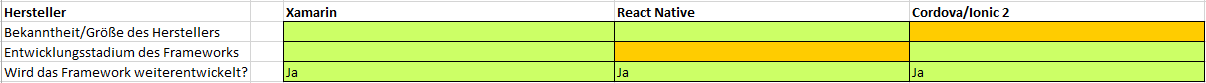
\includegraphics[width=1\textwidth]{Bilder/Auswertung_Hersteller.PNG}
	\caption{Bewertungsmatrix Kategorie Hersteller}
	\label{fig:AuswHerst}
\end{figure}

Wie man vielleicht schon anhand der engen Verknüpfung des Xamarin Frameworks mit der IDE 'Visual Studio' vermuten könnte, so steht hinter Xamarin Inc. der Hardware- und Software-Hersteller 'Microsoft'. Das Xamarin Framework befindet sich aktuell (Stand Februar 2017) in der Major-Version 'Cycle 9'. Es werden regelmäßig wöchentlich Releases herausgegeben. Die aktuellste unterstützte Android-Version ist die Version 7.1, welche auch die aktuellste Android-Version ist (Stand Februar 2017). Die aktuellste iOS-Version, für die mit dem Xamarin Framework entwickelt werden kann, ist die Version 10.4. Das Framework wird weiterentwickelt. 
\\
\\
Hinter dem Cordova-Framework steht der Software-Hersteller Apache. Das Ionic Framework ist das einzige Produkt des Unternehmens Drifty. Die Version 2 des Ionic Frameworks wurde am 25.01.2017 veröffentlicht. Sowohl vom Ionic Framework als auch vom Cordova Framework werden mehrere Releases pro Monat mit Neuerungen und Bugfixes herausgebracht. Beide Frameworks werden weiterentwickelt. 
\\
\\ 
Herausgeber des React Native Frameworks sind die Unternehmen Facebook und Instagram. Das Framework befindet sich aktuell (Stand Februar 2017) in der Version 0.42. Es befindet sich somit noch in einer Beta-Version. Entwicklern wird die Möglichkeit geboten sogenannte 'Feature Requests' zu stellen. Requests, die von genügend Entwicklern gewünscht werden, werden in die Planung der weiteren Entwicklung mit aufgenommen. Auf der Homepage des React Native Frameworks kann man einsehen, welche 'Feature Requests' sich momentan in der Umsetzung befinden. Seit Beginn 2017 werden zudem regelmäßige monatliche Releases veröffentlicht. 

\section{OS-Versionen}

Die Bewertung der einzelnen Frameworks in der Kategorie 'OS-Versionen' ist in nachfolgender Abbildung (X) dargestellt.

\begin{figure}[h]
	\centering
	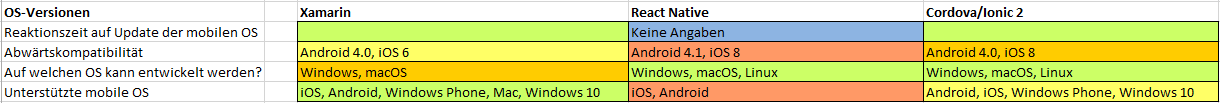
\includegraphics[width=1\textwidth]{Bilder/Auswertung_OSVersionen.PNG}
	\caption{Bewertungsmatrix Kategorie OS-Versionen}
	\label{fig:AuswOSVersionen}
\end{figure}

Zwischen dem Android-Update auf die Version 7.1 am 4.10.2016 und dem Update des Xamarin Frameworks für die Android-Version 7.1 am 19.10.2016 lagen knapp mehr als 2 Wochen.
\\
Auf das Android-Update auf die Version 7.1 am 4.10.2016 hat Xamarin gute 2 Wochen später am 19.4.2017 mit einem Update reagiert.
\\
Zur Abwärtskompatibilität lässt sich sagen, dass mit dem Xamarin Framework für Android-Geräte ab Version 4.0, für Apple-Geräte ab Version iOS6 und für Windows Phone ab Windows Phone 7 entwickelt werden kann. Bei Windows Phone 7-Anwendungen muss allerdings auf die Verwendung von Xamarin.Forms verzichtet werden.

\section{Funktionsumfang}

Die ausgefüllte Bewertungsmatrix für die Kategorie 'Entwicklung' ist in nachfolgender Abbildung (X) dargestellt.

\begin{figure}[h]
	\centering
	\includegraphics[width=1\textwidth]{Bilder/Auswertung_Funktionsumfang.PNG}
	\caption{Bewertungsmatrix Kategorie Funktionsumfang}
	\label{fig:AuswFunktion}
\end{figure}

Wie schon in Kapitel (X) erwähnt, bietet die API von Xamarin Zugriff auf alle Funktionalitäten, die eine native Android Anwendung auch bietet. Alle Sensoren können ausgelesen werden, Kommunikation via WiFi und Bluetooth ist möglich und eine mit Xamarin geschriebene Anwendung kann Notifications auslösen. Zudem kann auf die native Kamera-Anwendung von Android zugegriffen werden, die alle gebräuchlichen Kamerafunktionen wie Blitz und Kamerawechsel integriert hat. Dateien wie Fotos können an verschiedenen Speicherorten des Smartphones abgelegt werden. 
\\
\\
Bei der Kombination der Frameworks Cordova mit Ionic 2 fehlen noch Schnittstellen zu Barometer-, Näherungs- und Umgebungslichtsensor-Plugins in der Ionic 2 \textit{native}-Bibliothek. Wie schon in Kapitel (X) beschrieben, können trotzdem mit Mehraufwand Plugins eingebunden werden, die diese Sensoren ansprechen können. Wie bei dem Xamarin Framework kann auch mit Ionic die native Android Kamera-Anwendung in die eigene Anwendung integriert werden. Kommunikation via WiFi und Bluetooth sowie Zugriffe auf das Dateisystem und Notifications sind ebenfalls möglich. 
\\
\\
Außer der Nutzung des Barometers, zu der keine Informationen gefunden wurden, ist das Auslesen aller anderer in der Bewertungsmatrix (Abbildung (X)) gelisteten Sensoren mit dem React Native Framework umsetzbar. Sowohl auf die Front- als auch auf die Rückkamera eines Smartphones kann zugegriffen werden. Allerdings ist ein Aufruf der nativen Android-Kameraanwendung nicht in der API des Frameworks integriert, so muss eine Kameraanwendung mit allen Einstellungsmöglichkeiten selbst implementiert werden. Wie schon bei Xamarin und Ionic sind auch mit React Native Kommunikation via Bluetooth und Wifi sowie auch Notifications möglich. 

\section{GUI-Design}

\section{Interoperabilität}

Die Bewertung der einzelnen Frameworks in der Kategorie 'Interoperabilität' ist in nachfolgender Abbildung (X) dargestellt.

\begin{figure}[h]
	\centering
	\includegraphics[width=1\textwidth]{Bilder/Auswertung_Interoperabilitaet.PNG}
	\caption{Bewertungsmatrix Kategorie Interoperabilität}
	\label{fig:AuswInterop}
\end{figure}

Mit dem Xamarin Framework sind Webservice-Aufrufe umsetzbar und Drittanbieter-Bibliotheken können laut Xamarin in eine Anwendung eingebunden werden. Möchte man für seine Entwicklung das Xamrin Framework einsetzen, so muss auf einem Windows-PC mit der IDE 'Visual Studio' gearbeitet werden. Auf einem Apple-Computer ist das 'Xamarin-Studio' verpflichtend. 

\section{Tests}

\section{Performance}

\section{Programmiersprache}

\section{Sicherheit}


\newpage
\printbibliography

%\section*{Literaturverzeichnis}

\end{document}